\documentclass[a4paper,titlepage,bibliography=totoc]{scrreprt}

%==========================Bindekorrektur Option, oben in Documenclass hinzufügen===========
%,BCOR=15mm

%===========================PRÄAMBEL===============================
% Packages
%\usepackage[left=3cm,right=4cm,top=3cm,bottom=6cm]{geometry}
\usepackage[ngerman]{babel}
\usepackage[utf8]{inputenc}
\usepackage[T1]{fontenc}
\usepackage{setspace}
\setstretch{1,3}
\usepackage{array}
\usepackage{tabularx}
\usepackage{hyperref}
\usepackage{nameref}
\usepackage{graphicx}
\usepackage{epstopdf}
\usepackage{tikz}
\usepackage{color}
\usepackage{algorithmic}
\usepackage[absolute,overlay]{textpos}
\usepackage{babelbib} 
\usepackage{titleref}
\usepackage[colorinlistoftodos, textwidth=2cm, shadow, textsize = tiny]{todonotes}

%\setlength{\marginparwidth}{3cm}
%\usepackage{amsmath,amssymb,amsthm,amsfonts}
%\newcommand{\changefont}[3]{\fontfamily{#1} \fontseries{#2} \fontshape{#3} \selectfont}
%\usepackage{array}
%\usepackage{calc}
%\usepackage{scrlayer-scrpage}
%\usepackage{tabularx}
%\addtokomafont{caption}{\scriptsize} 

%===>Trennungsregeln für das gesamte Dokument.

%
%%% Trennungsregeln für das gesamte Dokument.
%
\hyphenation{da-bei}
\hyphenation{ge-schlos-sen-er}
\hyphenation{ent-spre-chen}
\hyphenation{lie-gen}
\hyphenation{Ge-sichts-ver-fol-gung}
\hyphenation{Re-prä-sen-tat-ion}
\hyphenation{pe-ri-phe-ren}
\hyphenation{an-ge-nom-me-ne}
\hyphenation{ge-speich-ert}
\hyphenation{ü-ber-nimmt}
\hyphenation{spei-chert}
\hyphenation{Schwan-kun-gen}
\hyphenation{Be-we-gungs-lo-sig-keit}
\hyphenation{be-reits}
\hyphenation{eu-kli-di-sche}
\hyphenation{ver-gleichs-wei-se}
\hyphenation{Im-ple-men-tier-un-gen}
\hyphenation{Haupt-auf-ga-be}
\hyphenation{dy-na-misch-es}
\hyphenation{ge-ne-rie-ren}
\hyphenation{aus-schließ-lich}
\hyphenation{auf-wei-sen}
\hyphenation{ge-ne-rie-ren}
\hyphenation{Zu-sam-men-set-zung}
\hyphenation{di-gi-ta-len}
\hyphenation{Mensch}
\hyphenation{Farb-ver-ständ-nis}
\hyphenation{Farb-wer-te}
\hyphenation{HSV-Farbraum}
\hyphenation{Schät-zung}
\hyphenation{kon-kur-rier-en-de}
\hyphenation{Ite-ra-ti-on}
\hyphenation{ge-samt-en}
\hyphenation{wis-sen-schaft-lich-en}
\hyphenation{di-gi-tal-en}
\hyphenation{Ma-schi-ne}
\hyphenation{Mo-dell}
\hyphenation{Be-wer-tungs-funk-tion}
\hyphenation{wel-ches}
\hyphenation{ganz-heit-liche}
\hyphenation{Be-ob-ach-tungs-me-cha-nis-mus}
\hyphenation{rgb-Farb-raum}
\hyphenation{Greif-be-we-gung-en}
\hyphenation{gauß-verteilt}
\hyphenation{auf-zu-füh-ren}
\hyphenation{hu-ma-no-i-den}
\hyphenation{O-ber-kör-per-Ver-fol-gung}
\hyphenation{ge-tes-te-ten}
\hyphenation{re-prä-sen-tiert}
\hyphenation{schlech-te-res}
\hyphenation{be-kann-ten}
\hyphenation{hoch-wer-ti-ge}
\hyphenation{ent-sprech-en-den}
\hyphenation{pro-blem-spe-zi-fisch-en}
\hyphenation{ein-ge-gang-en}
\hyphenation{ver-glei-che}
\hyphenation{Farb-zu-sam-men-setz-ung}
\hyphenation{Farb-raum}
\hyphenation{be-wer-ten}
\hyphenation{glo-ba-le}
\hyphenation{Be-wer-tung-en}
\hyphenation{Kon-fi-gu-ra-ti-ons-räu-men}
\hyphenation{Film-in-dus-trie}
\hyphenation{durch-zu-füh-ren}
\hyphenation{aus-ge-stat-et}
\hyphenation{igno-rie-ren}
\hyphenation{be-zeich-net}
\hyphenation{Ver-bin-dung}
\hyphenation{aus-zu-füh-ren}
\hyphenation{In-for-ma-ti-on-en}
\hyphenation{ent-wi-ckelt}
\hyphenation{Brenn-weite}
\hyphenation{Hin-ter-grund-ele-mente}
\hyphenation{ei-ner}
\hyphenation{be-stimmt}
\hyphenation{geo-me-trisch-e}
\hyphenation{be-schrie-ben}
\hyphenation{be-schrei-ben}
\hyphenation{be-stimmt}
\hyphenation{be-schreibt}
\hyphenation{Wahr-schein-lich-keits-funk-ti-on-en}
\hyphenation{Wahr-schin-lich-keits-funk-ti-on}
\hyphenation{mar-ker-lo-sen}
\hyphenation{Re-chen-leis-tung}
\hyphenation{Ste-re-o-ka-me-ra}
\hyphenation{In-te-res-se}
\hyphenation{Schwell-wer-tes}
\hyphenation{Kopf-po-si-ti-on-en}
\hyphenation{un-ter-such-ten}
\hyphenation{hie-rar-chi-sche}
\hyphenation{ge-gen-sei-tig}
\hyphenation{fin-det}
\hyphenation{be-trach-tet}
\hyphenation{Be-ob-ach-tungs-sche-ma}
\hyphenation{Ro-bo-ters}
\hyphenation{er-mög-lich-en}
\hyphenation{grei-fen-de}
\hyphenation{lin-ker}
\hyphenation{ge-spei-chert}
\hyphenation{drei-di-men-sio-na-len}
\hyphenation{Be-fin-den}
\hyphenation{dar-ge-stellt}
\hyphenation{müs-sen}
\hyphenation{be-stimmt}
\hyphenation{Si-tu-a-tio-nen}
\hyphenation{des-halb}
\hyphenation{letz-ten}
\hyphenation{Zu-fals-wer-tes}
\hyphenation{mö-gli-che}
\hyphenation{er-wei-tert}
\hyphenation{durch-schnitt-lich}
\hyphenation{Ro-bo-ter-kopf}
\hyphenation{schluss-end-lich}
\hyphenation{Farb-wahr-schein-lich-keits-ver-tei-lung} 


%===> Config
\graphicspath{{./Bilder/}}

\newcommand{\myname}{Peter Michael Bolch}
\newcommand{\mymanr}{1345211}
\newcommand{\mytitle}{Analyse internationaler Nachrichtenflüsse
im Twitter-Netzwerk}
\newcommand{\mysubmissiondate}{2014}
\newcommand{\myadvisor}{Matthias Keller}
\newcommand{\myprofessor}{Lehrstuhl \\ Prof. Dr. Hannes Hartenstein}
\newcommand{\myinstitute}{Dezentrale Systeme und Netzdienste\\ Institut für Telematik }
\newcommand{\myfaculty}{Fakultät für Informatik}
\newcommand{\myseminar}{Diplomarbeit}
\newcommand{\myseminardate}{2014}

%==============================================================================

% Macros
\newcommand{\name}[1]{\textit{#1}}
\newcolumntype{C}{>{\centering\arraybackslash}p{2em}}
% \renewcommand{\floatpagefraction}{.7}

%==============================================================================

\begin{document}

%=======================TITLEPAGES=============================================

%\newgeometry{left=2cm,top=2cm}
\pagestyle{empty}
% coordinates for the background shape on the titlepage
\newcommand{\diameter}{20}
%\newcommand{\xone}{-40}
\newcommand{\xone}{-20}
\newcommand{\xtwo}{480}
\newcommand{\yone}{50}
\newcommand{\ytwo}{-710}


\begin{titlepage}

% [ Rahmen ]
\begin{tikzpicture}[overlay]
\draw[color=gray]  
 		 (\xone pt, \yone pt)
  -- (\xtwo pt, \yone pt)
 arc (90:0:\diameter pt) 
  -- (\xtwo + \diameter pt , \ytwo pt) 
	-- (\xone + \diameter pt , \ytwo pt)
 arc (270:180:\diameter pt)
	-- (\xone pt, \yone pt);
\end{tikzpicture}

% [ Logo ]
%\begin{textblock}{10}[0,0](1.7,1.125)
\begin{textblock}{10}[0,0](2.0,1.125)
	
\includegraphics[width=.3\textwidth]{KITLogo_RGB.pdf}
\end{textblock}

  
  \begin{center}
    \begin{tabular}{r|l}
%	
\includegraphics[width=.3\textwidth]{KITLogo_RGB.pdf}
%      \includegraphics[width=1.5cm]{BILDER/iprlogo} 
& 
      \begin{minipage}{8cm} 
        \begin{large} \myinstitute \\
          \\
          \myprofessor \\
          \\
          \myfaculty \\
        \end{large}
      \end{minipage} \\
      % \hline
%      \multicolumn{2}{l}{
%       \begin{minipage}{7.5cm}
%          \vspace{.3cm}
%          \makebox{ \large 
%            Universit\"at Karlsruhe,
%            Fakult\"at f\"ur Informatik} \\
%        \end{minipage}
%      } \\
      \begin{minipage}{5cm}
        \begin{flushright}
          \vspace{4cm}
          \myseminar \\
          \myseminardate
        \end{flushright}
      \end{minipage}
      &\\
      & 
      \begin{minipage}{8cm}
        \vspace{-0.7cm}
        
        \begin{center}
          \begin{minipage}{8cm}
            \begin{flushleft}
              
                \mytitle\\[1cm]
                \myname \\[.5cm]
                
              
              Mat.Nr.: \mymanr
              \vspace{3cm}
            \end{flushleft}
          \end{minipage}
        \end{center}
        \vspace{4cm}
      \end{minipage}  \\
      & Referent:  \\
       & Betreuer: \myadvisor
    \end{tabular}
  \end{center}

\begin{textblock}{10}[0,0](1.75,15.365)
\tiny{ 
KIT -- Universit\"at des Landes Baden-W\"urttemberg und nationales Forschungszentrum der Helmholz-Gesellschaft
}
\end{textblock}

\begin{textblock}{10}[0,0](12,15.36)
\normalsize{
	\textbf{www.kit.edu} 
}
\end{textblock}

  
\end{titlepage}
\clearpage


		% Titelseiten Datei einbinden
%\restoregeometry
\vspace*{32\baselineskip}
\hbox to \textwidth{\hrulefill}
\par
\hfill \newline
Ich erkläre hiermit, dass ich die vorliegende Diplomarbeit selbständig verfasst und
keine anderen als die angegebenen Quellen und Hilfsmittel verwendet habe.
\hfill \newline \newline
Karlsruhe, \mysubmissiondate
\hfill
\myname

\clearpage

\pagestyle{plain} 

%=======================INHALTSVERZEICHNIS======================================
\pagenumbering{roman}	% römische Ziffern für das Inhaltsverzeichnis
\setcounter{page}{1}
%%%%%%%%%%%%%%%%%%%%%%%%%%%%%%%%%%%%%%%%%%%%%%%%%%%%%%%%%%%%%%%%%%%%%%%%%%%%%%%
%\begin{center}
%\begin{minipage}{10cm}
%\em
%{\bf Kurzfassung:} 
%\end{minipage}
%\end{center}
%\vspace{3cm}

\tableofcontents
%\listoftodos

\clearpage
%\pagestyle{empty}
\pagenumbering{arabic} % ab hier: Seitennummerierung in arabischen Ziffern
\clearpage

%!TEX root = ../document.tex
\chapter{Einleitung}\label{chp:Einleitung}

	\section{Motivation und Hintergründe}

		Über den Mikroblogging-Dienst Twitter lassen sich in Echtzeit 140 Zeichen lange Textnachrichten veröffentlichen.
		Seit dem Start des Mikroblogging-Dienstes im Jahr 2006 sind die Nutzerzahlen kontinuierlich angestiegen.
		2010 konnte Twitter 75 Millionen aktive Nutzer verzeichnen \cite{Cheng2010}.
		Im Jahr 2013 wird Twitter täglich von zirka 100 Millionen Menschen weltweit aktiv genutzt.
		Dies berichtete Twitter 2013 in seinem Prospekt zum Börsengang \cite{twitterinc2013}.  
		Zur Gesamtanzahl der Nutzer-Konten gibt es von Twitter keine Informationen. 
		Dies kann mitunter damit begründet werden, dass die Gesamtanzahl der Nutzer-Konten auch inaktive Nutzer einschliesst und somit keine Informationen über die tatsächliche Aktivität im Netzwerk liefert. 
		Auch andere soziale Netzwerke ziehen die aktiven Nutzer als Metrik heran, des weiteren wird die Metrik vom Interactive Advertising Bureau (IAB) empfohlen. \cite{IAB}
		
		Die Twitter-Nutzer verfassen täglich mehr als 500 Millionen Nachrichten, sogenannte Tweets \cite{twitterinc2013}. \footnote{Im Abschnitt Grundlagen wird der Begriff Tweet genauer untersucht, für den Moment sollen darunter die Nachrichten verstanden werden, welche von den Twitter-Nutzern verfasst werden}
		Die meisten dieser Tweets sind öffentlich zugänglich und können von allen Twitter-Nutzern uneingeschränkt betrachtet werden. 
		Twitter bietet zusätzlich eine sogenannte Streaming-API an, welche es ermöglicht Tweets programmatisch zu empfangen. \footnote{API: Application Programming Interface oder auch Programmierschnittstelle}
		Die Streaming-API stellt ein Echtzeit-Sample der aktuell versendeten Tweets bereit und liefert maximal 1\% aller Tweets die zum aktuellen Zeitpunkt verfasst wurden \cite{Morstatter2013}. 
		Über die sogenannte Filter-API lassen sich die Tweets nach bestimmten Kriterien wie Nutzer-ID, geografischer Region oder Schlüsselwörtern filtern.
		 \footnote{https://dev.twitter.com/docs/streaming-apis} 

		Ein Tweet besteht aus einer Reihe von Informationen.
		Neben dem Verfasser, ist der Tweet-Text die wichtigste Information die in einem Tweet enthalten ist.  
		Der Tweet-Text wird vom Nutzer verfasst und abgesendet, er beinhaltet die zentrale Information eines Tweets. 
		In den 140 Zeichen des Tweet-Textes teilen Twitter-Nutzer Informationen unterschiedlicher Ausprägung aus.
		Unter anderem wird über privates, Sportergebnisse, Großereignisse, persönliche Erfahrungen oder persönliche Meinungen berichtet. 
		Auch Bilder und Web-Links können in einem Tweet-Text enthalten sein. 

		Mit Hilfe der Streaming-API ist es erstmals möglich, große Mengen nutzergenerierter Informationen unterschiedlichster Ausprägung direkt zu erhalten. 
		Durch die Möglichkeiten die Twitter bietet kann theoretisch jeder Mensch Nachrichten und Informationen über das Twitter-Netzwerk verbreiten und weitergeben. 
		Diese Masse an nutzergenerierten Informationen bietet Wissenschaftlern in verschiedenen Bereichen zahlreiche neue Möglichkeiten.

		Sakaki et al interpretieren die Twitter-Kurznachrichten beispielsweise als Sensor-Daten \cite{Sakaki2010}.
		Der Twitter-Nutzer fungiert dabei als Sensor, der ein beliebiges Ereignis erfährt oder erlebt.
		Möglicherweise berichtet der Twitter-Nutzer im Tweet-Text über dieses Ereignis. 
		Damit kann der Text als Sensor-Datum interpretiert werden, wenn auch erhebliches Rauschen in der Gesamtheit der Tweets zu erwarten ist.    
		Sakaki et al zeigen aber, dass mit diesem Vorgehen, Erdbebenzentren lokalisiert oder die Trajektorie eines Typhoons vorhergesagt werden können.  \todo{Bild Twitter-Nutzer als sensor} 
		
		Auch die Sozialwissenschaften und die Meinungsforschung profitieren von dem enormen Informationsfundus der durch Twitter geboten wird.  
		Tumasjan et al. untersuchen in \cite{Tumasjan2011} wie sich die politische Landschaft im Twitter-Netzwerk wiederspiegelt. 
		Die Wissenschaftler haben zur Bundestagswahl 2009 100.000 Tweets analysiert und stellten fest, dass die Erwähnungen von Parteien und Politikern in Twitter, den Wahlausgang sehr genau wiederspiegelten.  
		
		Die Kommunikation innerhalb des Twitter-Netzwerks kann aber auch neue Einsichten über die globale Kommunikation oder die Ausbreitung von Nachrichten liefern.
		Garcia-Gavilanes et al. erforschen in \cite{Garcia-Gavilanes2014} die Kommunikation zwischen Ländern. 
		Es wird gezeigt, dass die globale Kommunikation innerhalb des Twitter-Netzwerks nicht nur von der geografischen Distanz abhängig ist, sondern auch von sozialen, ökonomischen und kulturellen Attributen eines Landes.   

		Selbst die Epidemieforschung kann von den Daten des Twitter-Netzwerks profitieren. 
		So zeigten Szomsor et al. in \cite{Szomszor2011}, dass die Vorhersage der Schweingrippe im Jahr 2009 durch die Analyse von Tweets eine Woche früher möglich gewesen wäre als dies mit konventionellen Frühwarnsystemen der Fall war. 

		Diese Erkenntnisse und Informationen sind allerdings nur gewinnbringend einzusetzen, wenn der Standort des Twitter-Nutzers bekannt ist. 
		Die Information, dass eine Krankheit ausgebrochen ist, ist mit einer exakten Georeferenz wertvoller als ohne diese. 
		Auch die Arbeit von Sakaki et al. ist auf eine Georeferenz angewiesen, wobei die Wissenschaftler angeben, dass die ungefähre Position für ihre Anwendung ausreichend ist.
		Bei der Untersuchung internationaler Kommunikation wiederum, ist es wichtig zu Wissen in welchem Land ein Tweet verfasst wurde.
		In diesem Fall kann die Georefrenz eine größere Region umfassen und muss nicht GPS-Genauigkeit aufweisen.  
		Wohingegen eine detaillierte Untersuchung des politischen Klimas innerhalb Deutschlands eine Auflösung auf Bundesländer-Ebene erforderlich machen würde. 

 		Twitter bietet seinen Nutzern die Möglichkeit ihren Standort im Nutzerprofil anzugeben. 
 		Hecht et al. stellen in \cite{Hecht2011} eine erste ausführliche Analyse der eingegebenen Standort-Daten bereit.  
 		Ab 2009 ermöglichte Twitter ein "'per-tweet geo-tagging"' \cite{Cheng2010}.
 		Dadurch können Anwendungen, auf Endgeräten mit GPS, Längen- und Breitengrad des aktuellen Standorts als Georeferenz an den Tweet anhängen.    
		Nur ca. 1,7\% der Twitter-Kurznachrichten enthalten allerdings eine konkrete Georeferenz in dieser Form. \footnote{Prüfung durch Datensatz XYZ was sich mit den Ergebnissen von \cite{Priedhorsky2013} und \cite{Schulz2013}}


	\section{Problembeschreibung} 
		Um gewinnbringende Informationen aus den Tweets erzeugen zu können, ist es wichtig Tweets eine Georeferenz zuordenen zu können.
		Die Anzahl der Twitter-Kurznachrichten die mit Hilfe von Längen- und Breitengrad unmittelbar einem geografischen Ort zugeordnet werden können ist sehr gering. 
		
		Es ist also wichtig ein Verfahren zu finden um Twitter-Nutzer oder Tweets eine Georeferenz zuzuordnen. 
		Mit Hilfe der in einem Tweet vorhandenen Daten sollte eine möglichst genaue Position bestimmt werden. 
		Dies soll auch möglich sein, wenn keine konkrete geografische Angabe in Form von Längen- und Breitengrad vorliegt. 

	\section{Fragestellungen und Anforderungen}\label{sec:fragestellung}
		Die folgenden Fragestellungen sollen beantwortet: 
		\begin{enumerate}
			\item[Q1] Wie kann Twitter-Nutzern eine Georeferenz zugeordnet werden?
		\end{enumerate}
		  
	\subsection{Anforderungen}\label{sec:Anforderungen}
	Das erarbeitete verfahren soll folgende Anforderungen erfüllen.
		\begin{enumerate}
			\item[R1] Zuordnung einer Georefrenz zu einem Twitter-Nutzer. (R1) 
			\item[R2] Unabhängig von kommerziellen Anbietern geografischer Informationen, oder sonstiger benötigter Daten. (R2)
			\item[R3] Das Ergebniss ist eine Georeferenz welche einer geografischen Hierarcheiebene enstpricht. Folgende Hierarcheiebenen werden angeboten (R3): 
			\begin{enumerate}
			 	\item Land oder Staat
			 	\item Verwaltungsebene erster Ordnung \footnote{in D Bundesländer, bspsw. Baden-Württemberg, Bayern usw. }
			 	\item Verwaltungsebene zweiter Ordnung \footnote{in D Regierungsbezirke bspsw. Regierungsbezirk Stuttgart, Regierungsbezirk Karlsruhe usw.}
			 	\item Stadt
			 \end{enumerate} 
			\item[R4] Es soll möglich sein eine Mindestanforderung für die Konfidenz, mit welcher die Georeferenz bestimmt wurde, anzugeben.  
			\item[R5] Verfahren unabhängig von Sprache und Schriftzeichen weltweit einsetzbar.
		\end{enumerate}
		
	\section{Gliederung der Arbeit}

		\subsection*{Abschnitt 2: Grundlagen}
			In diesem Abschnitt sollen die Grundlagen für die entwickelte Methode vermittelt werden. 
			Es wird auf den Mikroblogging-Dienst Twitter eingegangen und es werden grundsätzliche Methoden und Verfahren vorgestellt welche zum Verständnis der entwickelten Methode benötigt werden. 
			Ebenso werden häufig genutzte geografische Grundbegriffe vermittelt.

		\subsection*{Abschnitt 3: Stand der Technik}
			Es werden aktuelle Ansätze betrachtet, eingeordnet und in Bezug auf die angegebenen Anforderungen untersucht.
			Es werden sowohl die Verfahren zur '"Analyse'" und Zuordnung als auch die Verfahren zum abbilden der geografischen Einheiten untersucht und eingeordnet. 

		\subsection*{Abschnitt 4: Lösungsansatz}
			In diesem Kapitel wird, unter Berücksichtigung der gegebenen Anforderungen, ein Verfahren zur Lösung der Fragestellungen entwickelt. 
			Um einen Überblick zu gewährleisten, wird das Verfahren zunächst allgemein betrachtet, danach wird jeder Verfahrensschritt dargelegt.
			Es wird gezeigt wie aus Tweet-Daten der Standort eines Twitter-Nutzers bestimmen werden kann.
			Dabei werden Methoden der Sprachverarbeitung, Statistik und geografische Hierarchien eingesetzt. 

			Bottom-Up:

			\begin{enumerate}
				\item NGramme aus Indikatoren erzeugen
				\item Geomapping
				\item Datenstruktur
				\item Treffer zählen (NGramm + Geoid gleich usw.)
				\item Geografische Hierarchiebene
				\item Unsicherheit bei Lokalisierung messen (neuer Daten) 
				\item Justierung der Lokalisierungsunsicherheit auf geografischen Hierarchiebenen
			\end{enumerate}

		\subsection*{Abschnitt 5: Referenzimplementierung der entwickelten Methode}
			Es werden ausgewählte Auszüge, Probleme und Fallstricke der Referenzimplementierung erläutert und erklärt. 

		\subsection*{Abschnitt 6: Leistungsbewertung der entwickelten Methode}
			In diesem Kapitel werden die Ergebnisse der Refernzimplementierung bewertet und, soweit sinnvoll, gegenüber bestehenden Ansätze einer kritischen Betrachtung unterzogen. 

		\subsection*{Abschnitt 7: Schlussfolgerungen}
			Unter besonderer Berücksichtigung der Ergebnisse des letzten Kapitels werden Schlussfolgerungen gezogen. 
			Der Beitrag und nutzen der entwickelten Methode soll kritisch hinterfragt werden.

		\subsection*{Abschnitt 8: Zusammenfassung und Ausblick}
			Zusammenfassung der Arbeit und kritischer Rückblick. Im Ausblick werden mögliche Verbesserungen und Ideen zur Weiterentwicklung gegeben.  

%!TEX root = ../document.tex
\chapter{Grundlagen} 
Um die Fragestellungen aus Abschnitt \ref{sec:fragestellung} beantworten zu können und eine geeignete Methode zu entwickeln um die Anforderungen zu erfüllen, werden eine Reihe von grundlegenden Verfahren und Begriffen verwendet. 
Der Leser soll hier auf einen Stand gebracht werden, der es ihm ermöglicht die Ausführungen und Ideen nachvollziehen zu können.  
Des weiteren wierden einige Grundlagen zu Twitter erklärt und die Daten, welche mit einem Tweet gesendet werden betrachtet.
Zum Schluss wird die genutzte Datenbasis und der Einfluss der von Twitter genutzten Sampling Strategie vorgestellt und erläutert.

\newpage

	\section{Geografische Grundlagen und Begriffe}
	In diesem Kapitel sollen geografische Grundbegiffe erläutert werden. 
	Einige geografische Begriffe werden in verschiedenen wissenschaftlichen Bereichen unterschiedlich genutzt und teilweise widersprüchlich definiert. 
	Um Missverständnissen vorzubeugen wird hier definiert was unter den einzelnen Begriffen genau zu verstehen ist.
	Eine Reihe von Begriffen werden selbst definiert um bestimmte Sachverhalte klarer ausdrücken zu können. 

		\paragraph*{Geodätisches Referenzsystem} 
		\todo{Referenz. MAtthias Fragen, Online Lexikon zu Geoinformatik Uni Rostock} 
		Ein geodätisches Referenzsystem dient als einheitliche Grundlage zur Angabe einer Position auf der Erde. 
		In diesem Referenzsystem werden unter anderem Referenzpunkte und ein geeignetes Koordinatensystem festgelegt.  
		
		\paragraph{Georeferenz}
		\todo{Referenz. MAtthias Fragen, Online Lexikon zu Geoinformatik Uni Rostock} 
		Eine Georeferenz (engl. Spatial Reference) wird auch als Raumbezug bezeichnet. 
		Unter dem Begriff der Georeferenz versteht man die zugeordnete der Lage beziehungsweise Position zu einem Datensatz. 
		Die konkreten Angaben zum Raumbezug und deren Genauigkeit hängen von den Anforderungen ab, die an die Georeferenz gestellt wird. 
		Auch die in Kapitel \ref{chp:Einleitung} erwähnten Anwendungen stellen unterschiedliche Anforderungen an die Genauigkeit der Georeferenz.
		Die Georeferenz lässt sich weiter unterteilen in:
		
			\begin{description}
	 			\item[Direkte Georeferenz (direkter Raumbezug)] 
	 			Unter direktem Raumbezug versteht man die Angabe einer konkreten Koordinate bezüglich eines geeigneten, unveränderlichen geodätischen Referenzsystems. 
	 			\item[Indirekte Georeferenz (indirekter Raumbezug) ] 
	 			Unter indirektem Raumbezug werden alle Angaben verstanden die eine ungenaue Position bezüglich eines beliebigen Referenzysystems bestimmen.
	 			Ungenau ist in dem Sinne zu verstehen, dass die Angabe der Position auch eine Fläche beschreiben kann.
	 			Zusätzlich muss das gewählte Referenzsystem nicht zwingenderweise unveränderlich sein.   
	 			Beispiele für die Angabe eines indirekten Raumbezugs wären Länder, Adressen, Postleitzahlen oder auch Telefonvorwahlen. 
	 			Alle diese Angaben, mit Ausnahme der Adresse, definieren eine geografische Fläche. 
	 			Diese Fläche ist nicht zwingenderweise klar abzugrenzen.
			\end{description}

	 	\paragraph*{Georeferenzierung}
		Unter Georeferenzierung versteht man die Zuordnung einer Georeferenz zu einem Datensatz. 
		Also den Vorgang einem Datensatz, zum Beispiel einem Twitter-Nutzer eine Georeferenz zuzuordnen.

	 	Aufrgund der einfacheren Verständlichkeit werden die folgenden zwei Begriffe definiert, welche in der restlichen Arbeit verwendet werden.

		\paragraph*{Geografische Position}
		Unter geografischer Position wird hier ein konkreter Ort, unter Angabe geografischer Koordinaten verstanden.
		Eine geografische Position entspricht somit einer direkten Georeferenz (direktem Raumbezug).

		\paragraph*{Geografische Region} 
		Unter einer geografischen Region werden Flächen verstanden welche nicht mit einem Punkt, in Form von Längen- und Breitengrad, beschrieben werden können. 
		Hierbei kann es sich beispielsweise um Bundesländer oder Länder.
		Somit entspricht der Begriff geografische Region einer indirekten Georeferenz (indirektem Raumbezug).

		\paragraph*{Geografische Hierarchien}
		\todo{Bild mit Hierarchie von Deutschland} 
		In der vorliegenden Arbeit werden geografische Hierarchien verwendet um eine Einteilung der Erde in geografische Regionen umzusetzen.
		Dabei können geografische Regionen wiederum geografische Regionen oder geografische Positionen enthalten, wodurch sich eine hierarchische Gliederung ergibt.
		Diese Einteilung spiegelt im wesentlichen die Einteilung der Erde in Staaten und deren individuellen Verwaltungseinheiten wieder.
		Im vorliegenden Fall ist das Staatsgebiet, also die Fläche über die sich der Staat erstreckt, von Interesse. \footnote{Die genaue Definition eines Staatsgebietes kann in \cite{jellinek1921} nachgelesen werden.} 

		Im Gegensatz dazu könnte die Erde auch in ein Gitternetz eingeteilt werden. 
		Die einzelnen Zellen würden dann als Referenz für eine geografische Region verwendet werden.
		Dieses vorgehen wird unter anderem in \cite{Serdyukov2009} angewendet.

		Eine Aufteilung der Erde in geografische Regionen lässt sich auf oberster Ebene mit Hilfe von Ländern und deren Grenzen umsetzen. 
		Daraus resultiert eine Einteilung, welche direkt intuitiv verständlich ist und vielen Anforderungen an geografische Informationen gerecht wird.
		Die meisten Länder sind in weitere administrative Einheiten aufgeteilt.
		Ausnahmen sind besipielsweise Stadtstaaten wie der Vatikan-Staat oder das Fürstentum Monaco, welche aufgrund ihrer Größe nicht in Verwaltungsbezirke unterteilt werden.
		Diese geografischen Regionen werden hier als Administartionsebenen bezeichnet.
		Es wird zwischen Administrationsebenen erster und zweiter Ordnung unterschieden. 
		Des weiteren werden Städte in der untersten Ebene der Hierarchie dargestellt.
		Wenn man als Beispiel Deutschland heranzieht, ergibt sich eine Einteilung wie in Bilde \todo{referenz auf Bilc}.
		Die oberste Ebene beschreibt das Land worauf die zweite Ebene die Bundesländer darstellt.
		Auf der dritten Ebene werden die Regierungsbezirke abgebildet, worauf die Städte in der letzten Ebene folgen. 
		Bis auf die letzte Ebene wird den Objekten in der Hierarchie eine geografische Region zugeordnet. 
		Lediglich die unterste Ebene, die der Städte wird durch eine geografische Position genau beschrieben. 
		Die Ausdehnung einer Stadt wird in der gegebenen Hierarchie also nicht berücksichtigt. 
		Jede Stadt beziehungsweise Stadtteile werden als konkrete geografische Koordinate in Form von Längen- und Breitengrad repräsentiert. 

	\section{Twitter} 
	In diesem Kapitel werden grundlegende Begriffe rund um das Twitter-Netzwerk erläutert. 
	Weiter werden die Mechanismen in Twitter erläutert und an praktischen Beispielen erklärt. 
	Zum Schluss wird aufgezeigt welche Informationen pro Twitter-Kurznachricht übermittelt werden und welche Daten zur Lokalisierung verwendet werden können.

	\subsection{Geschichtliches}
	Twitter wurde 2006 von Jack Dorsey, Biz Stone, Noah Glass und Evan Williams gegründet.
	Ursprünglich war Twitter zur internen Kommunikation innerhalb der Firma Odeo geplant.
	Schnell wurde allerdings klar, dass in dem Dienst mehr potenzial steckt und so wurde Twitter öffentlich gemacht.
	Seitdem erfreut sich der Dienst einer wachsenden Nutzer-Gemeinde.
	Die Twitter-Gründer haben von Anfang an keine exakten Nutzer-Zahlen oder die Anzahl der versendeten Twitter-Kurznachrichten bekanntgegeben.
	Dies geschah einerseits, weil die Gründer davon überzeugt sind, dass anhand der reinen Nutzer-Zahlen und gesendeten Twitter-Kurznachrichten nicht die '"Gesundheit"' des Twitter-Netzwerks nachvollzogen werden kann, andererseits werden durch diese Massnahme auch strategische Ziele verfolgt.  \footnote{http://www.pbs.org/mediashift/2007/05/twitter-founders-thrive-on-micro-blogging-constraints137}
	2013 ging Twitter an die Börse und vermeldete 100 Millionen täglich aktive Nutzer und über 500 Millionen Twitter-Kurznachrichten, die täglich über den Dienst versendet werden. 

	\subsection{Was ist Twitter?}
	Twitter wird als Kurznachrichten-Dienst, Mikroblogging-Dienst oder auch als soziales-Netzwerk bezeichnet. 
	Twitter Geschäftsführer Kevin Thau hat 2010 auf dem Nokia-World Kongress öffentlich bestritten, dass Twitter ein Soziales-Netzwerk ist. 
	Laut Thau handelt es sich um ein Nachrichten-, Inhalts- und Informations-Netzwerk. 
	Er begründete dies damit, dass Twitter die Art und Weise wie Nachrichten verteilt werden ändert und praktisch jeder zum Journalisten werden kann. 
	Als Beispiel nennt er die Landung des Fluges 1549 auf dem Hudson River, die Zeugen hätten keine Mails versendet um die Nachricht zu verbreiten, sondern die Nachricht via Twitter weitergegeben.
	Es lassen sich eine Reihe weitere Beispiele derselben Art finden. 
	In \cite{Kwak2010} wird diese Einschätzung wissenschaftlich bestätigt.
	Kwak et al überprüfen die in \cite{Newman2003} beschriebenen Eigenschaften sozialer Netzwerke und kommen zu dem Schluss, dass Twitter diese Eigenschaften nicht erfüllt.

	Twitter ermöglicht es den Nutzern 140 Zeichen lange Nachrichten, so genannte Tweets, zu erstellen. 
	Diese Tweets sind standardmäßig öffentlich sichtbar und werden als Liste in umgekehrter chronologischer Reihenfolge im Twitter-Profil dargestellt. 
	Damit hat das Twitter-Profil einen Blog Charakter.  
	In der vorliegenden Arbeit wird Twitter deshalb als Mikroblogging-Dienst bezeichnet.
	Die Bezeichnung Kurznachrichten-Dienst ist irreführend, da dieser mit sms (small messeneger service) in Verbindung gebracht werden kann. 
	Tatsächlich galt der sms in der Anfangsphase von Twitter als Vorbild für den Dienst.
	Die Darstellung als Liste, und die Funktion einen Tweet standardmäßig allen Nutzern freizugeben unterscheidet sich grundlegend von der Funktion des sms, bei dem eine Nachricht direkt an einen Empfänger gesendet wird und nicht öffentlich ist.

	\subsection{Funktionen von Twitter}
	Der Mikroblogging-Dienst Twitter bietet neben dem Profil, auf dem die Tweets des Nutzers angezeigt werden, noch eine Reihe weiterer Funktionen. 
	Im folgenden soll das Twitter-Profil und die Timeline kurz erläutert werden. 
	Danach werden Funktionen wie das weitergeben eines Tweets, Favorisieren und Antworten erklärt. 
	Zum Schluss wird auf den gesendeten Tweet Inhalt eingenagen und der Netzwerk-Charakter von Twitter untersucht.

	\begin{figure}[h!]
	\begin{center}
	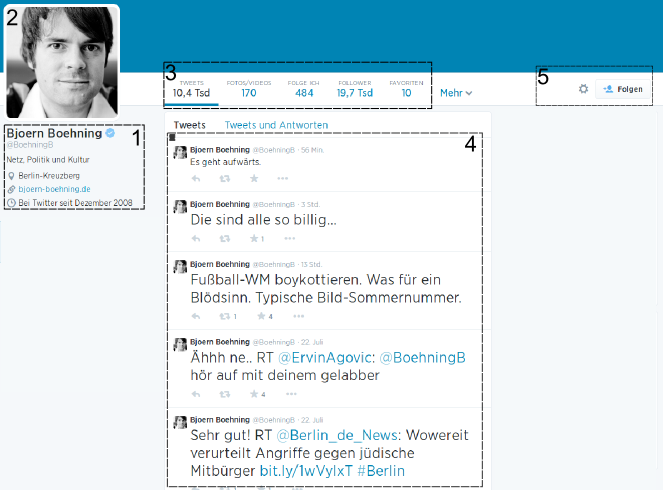
\includegraphics[scale=0.4]{profile.png}
	\caption{Die Twitter-Timeline auf einem Twitter Profil. 1: Nutzername und Informationen über den Nutzer. 2: Profilbild
	3: Allgemeine Informationen über den Benutzer und dessen Netzwerk
	4: Nutzer-Timeline: Tweets des Nutzer in umgekehrter chronologischer Reihenfolge 
	5: Button zum Folgen}
	\label{twitterProfile}
	\end{center}
	\end{figure}


		\paragraph{Das Nutzer-Profil und die Nutzer-Timeline}
			Das Nutzer-Profil kann über die Url http://twitter.com/BENUTZERNAME abgerufen werden und bietet neben der Nutzer-Timeline, in der die Tweets des Nutzers angezeigt werden, eine Reihe an weiteren Informationen.
			In Abbildung \ref{twitterProfile} ist in der mitte die Timeline des Benutzers dargestellt in der dei Tweets zu sehen sind. 
			Unter dem Profilbild links sind Informationen des Nutzers aufgelistet.
			Diese Informationen kann der Nutzer selbst einstellen und entscheiden welche er angeben möchte.   


		\paragraph{Folgen (Following/Follower/Tweeps)}
			Diese Funktion erlaubt es Tweets eines bestimmten Nutzers zu abonnieren. 
			Im Twitter-Umfeld spricht man von '"following"' oder '"folgen"', wenn man die Tweets eines bestimmten Nutzers abonniert.
			Hat man Tweets eines bestimmten Nutzers abonniert so wird man als dessen '"Follower"' bezeichnet. 
			Das englische Wort '"Follower"' hat sich im Twitter-Umfeld und darüber hinaus eingebürgert und wird selten übersetzt. 
			Auch auf der Twitter Website wird '"Follower"' nicht ins deutsche übersetzt.
			In der vorliegenden Arbeit wird deshalb auch auf eine Übersetzung verzichtet. 

			In Abbildung \ref{twitterProfile} an Position 3 wird unter '"Folge ich"' die Anzahl der Twitter-Nutzer angezeigt denen der Beispielnutzer folgt. 
			Neben dem Feld '"Folge ich"' wird unter '"Follower"' angezeigt wieviele Nutzer dem Beispielnutzer folgen.

		\paragraph{Netzwerk Charakter}
			Netzwerke in Twitter entstehen ausschliesslich durch Follower-Beziehungen.

		\paragraph{Persönliche Timeline}
			Jeder Twitter-Nutzer hat seine persönliche Timeline, auf dieser werden die Tweets derjenigen Nutzer angezeigt, denen er folgt. 
			Die Timeline kann als Aggregator für Tweets betrachtet werden.
			Diese Timeline ist die zentrale Stelle, an der die Nutzer Tweets anderer Nutzer empfangen und lesen.
			Auch hier werden die Tweets in umgekehrter chronologischer Reihenfolge angezeigt.  

		\paragraph{Weitergeben eines Tweets (Retweet)}
			Unter einem Retweet versteht man die Weitergabe eines Tweets den man nicht selbst verfasst hat an die eigenen Follower.
			Genauer gesagt wird der Tweet übernommen und ein Hinweis hinzugefügt, dass es sich um einen Retweet handelt, und nicht einen vom Nutzer selbst verfassten Tweet.
			Diese Funktion wird hauptsächlich genutzt um Nachrichten schnell zu verbreiten ohne diese neu eingeben zu müssen. 
			Die Weitergabe an die eigenen Follower impliziert einen gewissen Grad an Kontrolle und Filterfunktion.
			Der weitergebende Nutzer kontrolliert und filtert die Nachrichten die er erhält und gibt diejenigen weiter, denen er eine Gewisse Relevanz beimisst, oder von denen er erwartet, dass sie seine Follower interessieren. \todo{1 retweet Reichweite 1000 Nutzer} 
			Mit dieser Funktion können einzelne Nutzer eine Art Filterfunktion übernehmen, welche früher Journalisten vorbehalten war. 
			Auch können Nutzer dadurch zu Tweet-Aggregatoren werden, welche Tweets von mehreren Nutzern erhalten, aber nur relevante oder themenspezifische Tweets weitergeben.


			\todo{Diagramm Retweet, Filterfunktion} 


		\paragraph{Antworten und ansprechen eines Nutzers}
			Twitter bietet die Möglichkeit einzelne Nutzer direkt anzusprechen. 
			Mit Hilfe des @-Symbols kann ein Nutzer referenziert werden. 
			Der referenzierte Nutzer, besipielsweise @alfred, wird dann benachrichtigt, dass er in einem Tweet erwähnt wurde. 
			Der erwähnte Nutzer muss dabei nicht Follower des Verfassers sein.
			Eine weitere Funktion im Twitter-Netzwerk ist das Antworten auf einen Tweet.
			Über eine Schaltfläche kann man auf einen Tweet Antworten. 
			Das @-Symbol und der Nutzername des Verfassers, des Ursprungstweets werden automatisch eingetragen, womit eine Benachrichtigung erfolgt. 
			Auch kann dem Antwort-Tweet der ursprüngliche Tweet zugeordnet werden.
			Es ist möglich, das auf einen Antwort-Tweet wieder geantwortet wird, wodurch ein sigenannter Thread entsteht. 
			Auch ist es möglich, dass an einer solchen Konversation mehrere Twitter-Nutzer beteiligt sind. 
			Dies ist dann der Fall, wenn im ursprünglichen Tweet, auf den geantwortet wurde, auf weitere User referenziert wurde. 
			Aber auch wenn ein Nutzer auf einen bestheneden Antwort-Thread wiederum antwortet, werden alle beteiligtien Nutzer referenziert. 
			\todo{Diagramm Antwort, Antwort Thread, Bild Antwirten Button, Referenzieren}     


		\paragraph{Favorisieren}
			Mit dieser Funktion lässt sich ausdrücken, das man einen Tweet interessant oder gut findet.
			Auch Zustimmung wird durch favorisieren ausgedrückt.  
			Einen Tweet zu favorisieren kann aber auch bedeuten '"ich habe deine Reaktion registriert"', oft um einen Antwort-Thread nicht abrupt abzubrechen sondern eine zustimmende Rückmeldung zu geben ohne extra einen Tweet zu verfassen.

 		
	 	\paragraph{Tweets}
	 		Neben den sichtbaren Daten, welche in der Timeline angezeigt werden. 
	 		Enthält ein tweet eine reihe weiterer interessanter Informationen. 
	 		  
	 		
	 	\paragraph{}
	 	\begin{enumerate}
	 		 \item Anatomie eines Tweets 
					\begin{enumerate}
						\item Welche Informationen sind in einem Tweet enthalten? 
						\item Konzentration auf Daten die Hinweise zur räumlichen Lage geben könnten aber auch allgemein auf die Daten eingehen.
					\end{enumerate}
	 	\end{enumerate}
			

		\subsection{Twitter}
			Allgemeine Informationen zu Twitter. 
			\begin{enumerate}
			\item \todo{gesicherte und ungesicherte Geoniformationen definieren!} 
				\item Twitter als Nachrichtenmedium (Can Twitter Replace Newswire (Petrovic et. al ))
				

					\item Definition Twitter-Umfeld
			\end{enumerate} 



	\section{geografie Daten}


	\section{Data Sample}




\chapter{Stand der Technik} 
	Die Georeferenzierung von Twitter-Kurznachrichten oder Twitter-Nutzern ist ein Feld an dem nach wie vor aktiv geforscht wird.
	Nicht zuletzt trägt auch die große Verfügbarkeit an Twitter-Daten zu dem Umstand bei, dass Twitter in den letzten Jahren Forschungsgegenstand zahlreicher Publikationen war. 
	
	In diesem Abschnitt sollen bestehende Ansätze zur Georeferenzierung im Twitter-Umfeld untersucht werden. 
	Es werden Kriterien zur Einordnung der bestehenden Ansätze erarbeitet und erläutert.   
	Die Arbeiten werden mit Hilfe der Kriterien schematisch eingeordnet um einen Überblick zu erhalten. 
	Zum Schluss wird untersucht ob die Arbeiten die bereits formulierten Anforderungen aus \ref{sec:Anforderungen} erfüllen, und wie sich die vorliegende Arbeit von den bestehenden Ansätzen abgrenzt.    

		\section{Kategorisierung bestehender Ansätze}

		In früheren Arbeiten wurde bereits versucht, eine Einordnung der bestehenden Verfahren vorzunehmen. 
		Es ist interessant die Kategoriesierungsansätze und die verwandten Arbeiten einiger Autoren zu studieren.
		Es lässt sich dadurch die Entwicklung zum Thema Lokalisierung im Twitter-Umfeld beobachten. 
		Einige Kategorisierungsansätze werden im folgenden aufgelistet und erläutert.

		Sowohl in \cite{Hecht2011} als in \cite{Cheng2010} beschränken sich die verwandten Arbeiten nicht auf die Lokalisierung im Twitter-Umfeld, es werden Arbeiten zur Lokalisierung von Web-Inhalten im Allgemeinen aufgelistet. 
		Dies lässt darauf schliessen, dass sich vor den Jahren 2010/2011 nur wenige Arbeiten mit der Lokalisierung im Twitter-Umfeld beschäftigt haben.  
		
		\subsubsection{Kategorisierung über die untersuchte Ressource}
		\cite{Hecht2011} nimmt deshalb eine Kategorisierung anhand der untersuchten Ressource vor. 
		Es wird unterschieden zwischen Forschungen zur "'Lokalisierung von Microblogging-Seiten und deren Inhalten"' und der "'Lokalisierung von Nutzern, welche Inhalte zu Web 2.0 Seiten beisteuern"'. 
		Zusätzlich wird in dieser Arbeit das "'Verhalten der Nutzer im Umgang mit der Veröffentlichung ihres aktuellen Standorts"' und die "'Vorhersage privater Informationen"' betrachtet. Darauf soll hier allerdings nicht weiter eingegangen werden.      

		\subsubsection{Kategorisierung über die verwendete Methode}

		\cite{Cheng2010} klassifiziert die vorgestellten Arbeiten anhand der verwendeteten Methodik. 
		Es wird auf Arbeiten zur Lokalisierung von Webseiten, Web-Logs, Suchanfragen und Web-Nutzern verwiesen. 
		Diese werden in die folgenden drei Kategorien eingeteilt.

		\paragraph*{"'Inhaltsanalyse mit Begriffen in einem geografischen Verzeichnis (Content analysis with terms in a gazetteer)"'}  
		Es wird darunter eine einfache Datenbanksuche verstanden. 
		Es werden einzelne Wörter in einer Datenbank nachgeschlagen um diese einem konkreten geografischen Ort zuweisen zu können.
		Dabei kann sowohl lokal auf eine Geo-Datenbank als auch auf Internet Ressourcen zurückgegriffen werden.  
		In der Regel durchläuft der untersuchte Text eine manuelle oder automatische Vorverarbeitung um potenziell geografische Begriffe, sogenannte Toponyme, herauszufiltern. 

		\paragraph*{"'Inhaltsanalyse mit probabilistischen Sprachmodellen (Content analysis with probabilistic language models)"'}
		Dabei werden Texte oder Textteile einer Twitter-Kurznachricht zu vordefinierten geografischen Regionen wie Ländern oder Städten zugeordnet. 
		Nach einer Vorverarbeitung des Textes erfolgt eine statistische Auswertung, um danach den Text oder einzelne Textteile, wie beispielsweise Wörter, einer geografischen Region zuzuordnen. 
		Eine unbekannter Text kann dann mit Hilfe der zuvor gelernten Zuordnung einer geografischen Region zugeordnet werden.

		\paragraph*{"'Schlussfolgerungen durch soziale Verbindungen (Inference via social relations)"'} es werden soziale Verbindungen, die in Netzwerken abgebildet sind, herangezogen um Rückschlüsse auf den geografischen Ort des untersuchten Inhaltes oder einer Person ziehen zu können.

		Preidhorsky et al. schlagen in \cite{Priedhorsky2013} eine weitere Einteilung anhand der Methodik vor. 
		Allerdings werden hier ausschließlich Arbeiten im Twitter-Umfeld betrachtet. 

		\paragraph*{"'Geocoding"'} Im wesentlichen entspricht dies der "'Inhaltsanalyse mit Begriffen in einem geografischen Verzeichnis"' aus \cite{Cheng2010}. 
		"'Geocoding"' wird als Begriff in vielen Fachrichtungen unterschiedlich definiert, was zu Missverständnissen führen kann. 
		In \cite{bibsmaniaaa:Goldberg2008} wird genauer auf den Begriff des Geocoding und die Poblematik eingegangen und eine Definition  des Begriffs vorgeschlagen.
		Im vorliegenden Kontext ist es präziser und weniger missverständlich die Methodik als "'Inhaltsanalyse mit Begriffen in einem geografischen Verzeichnis"' zu bezeichnen, anstatt den Begriff "'Geocoding"' einzusetzen. 
		
		\paragraph*{"'Geografische Themenmodelle (geografic Topic Modeling)"'} wird definiert als die Verbindung von "'Themenmodellierung"' und "'Standorterkennung (Location Awareness)"'. 
		Durch klassisches "'Themenmodellierung"' lässt sich aus aus Texten eine Menge von Themen extrahieren. 
		Durch eine Lernphase werden Wörterbücher zu den Themen erstellt.
		Mit Hilfe dieser Themen-Wörterbücher kann später das Thema eines Textes bestimmt werden. \cite{Blei2012} 
		Unter "'Standorterkennung"' wird hier verstanden, dass nicht nur das Thema sondern auch eine bestimmte Region extrahiert werden kann. 
		Dies kann durch geografischen Koordinaten in Twitter-Kurznachrichten realisiert werden. 
		Im Unterschied zur Kategorie "'Inhaltsanalyse mit probabilsitischen Sprachmodellen"' aus \cite{Cheng2010} wird hier jedoch keine vorgegebene geografische Region gefordert. 
		Vielmehr ergeben sich die geografischen Regionen aus den Themenmodellen und den zugehörigen geografischen Koordinaten.
		Es wird damit eine kontinuierliche Region beschrieben, welche nicht zwangsweise durch Stadt-, Staaten- oder Ländergrenzen beschränkt ist.  

		\paragraph*{"'Statistische Klassifizierung (Statistical classifiers)"'} Diese Kategorie entspricht der "'Inhaltsanalyse mit probabilsitischen Sprachmodellen"' wobei in \cite{Cheng2010} nur eine Arbeit in dieser Kategorie betrachtet wird. \cite{Priedhorsky2013} listet mehrere Arbeiten auf, die sich in diese Kategorie einordnen lassen.   

		\paragraph*{"'Informationen aus sozialen Verbindungen (Social Network Information)"'} analog zu "'Schlussfolgerungen durch soziale Verbindungen"' aus \cite{Cheng2010} werden soziale Verbindungen herangezogen um den Standort zu bestimmen. 

		Priedhorsky et al. wählen eine ähnliche Einteilung wie vormals Cheng et al. in 2010, die verwandten Arbeiten stammen allerdings aus dem Twitter-Umfeld. 
		Dabei ist zu bemerken, dass sich die verwendeten Methoden zur Lokalisierung im Twitter-Umfeld nicht wesentlich von denen in anderen Bereichen unterscheiden. 
		Um die Arbeiten im Twitter-Umfeld sinnvoll voneinander abgrenzen zu können muss die Kategorisierung mehr Dimensionen umfassen. 
		Es müssen mehr Kriterien zur Kategorisierung herangezogen werden als die reine Methodik.   

		Mahmud et al. betrachten in \cite{Mahmud2012} hauptsächlich Arbeiten im Twitter-Umfeld. 
		Diese werden in die folgenden Kategorien unterteilt. 

		\begin{enumerate}
			\item  "'Inhaltsbasierte Standortschätzung von Tweets (Content-based Location Estimation from Tweets)"'
			\item "'Inhaltsbasierte Standortextrahierung von Tweets (Conetnt-based Location Extraction from Tweets"'
			\item "'Standortschätzung ohne den Tweet Inhalt zu nutzen (Location Estimation without using Tweets Content)"'
		\end{enumerate}

		\paragraph*{"'Inhaltsbasierte Standort-Schätzung von Tweets (Content-based Location Estimation from Tweets)"'} hier wird die geografische Position durch eine Inhaltsanalyse der Twitter-Kurznachricht geschätzt. 
		Die Schätzung erfolgt dabei durch probabilistische Modelle.
		Diese Kategorie vereint damit "'Geografische Themenmodelle"', "'Statistische Klassifizierung"' aus \cite{Priedhorsky2013} mit "'Inhaltsanalyse mit probabilsitischen Sprachmodellen"' aus \cite{Cheng2010} und ist damit als genereller anzusehen, als die vorgenannten Kategorien. 

		\paragraph*{"'Inhaltsbasierte Standort-Extrahierung von Tweets (Conetnt-based Location Extraction from Tweets"'} die verwandten Arbeiten in dieser Kategorie versuchen direkte Hinweise auf einen geografischen Ort aus einer Twitter-Kurznachricht zu extrahieren. 
		Diese Kategorie ähnelt dem "'Geocoding"' beziehungsweise der "'Inhaltsanalyse mit Begriffen in einem geografischen Verzeichnis"'. 

		\paragraph*{"'Standortschätzung ohne den Tweet Inhalt zu nutzen (Location Estimation without using Tweets Content)"'} hierunter versteht der Autor alle Informationen die nicht unmittelbar in der Twitter-Kurznachricht enthalten sind. Dazu zählen Informationen aus dem Nutzerprofil oder Informationen über die sozialen Verbindungen des Nutzers.


		\cite{Mahmud2012} nutzt ebenfalls die Methodik um die Arbeiten zu kategorisieren. 
		Allerdings wird hier eine generellere Einteilung vorgenommen. 
		So wird unterteilt, ob der Standort geschätzt oder extrahiert wurde.  
		Mahmud et al. bringen aber auch eine weitere Dimension ein. 
		Es wird hier zusätzlich unterschieden ob das angewendete Verfahren den Tweet-Inhalt nutzt oder andere Informationen. 

		Dies ist sinnvoll, denn die genannten Methoden lassen sich sowohl auf den Tweet-Inhalt als auch auf andere Informationen, beispielsweise aus dem Nutzerprofil, anwenden. 
		
		Frühere Arbeiten verweisen auf ein weiteres Spektrum an Arbeiten aus anderen Bereichen, wie Lokalisierung von Flickr Bildern oder Web-Log Einträgen.
		Arbeiten zur Lokalisierung im Twitter-Umfeld werden hier seltener erwähnt. 
		In späteren Arbeiten, wie in \cite{Priedhorsky2013}, wird hingegen fast ausschließlich auf Arbeiten aus dem Twitter-Umfeld verwiesen. 
		Dies spiegelt die steigende Anzahl der Arbeiten zur Lokalisierung im Twitter-Umfeld wieder.
		Betrachtet man die Ausarbeitungen zur Lokalisierung im Twitter-Umfeld genauer, wird allerdings schnell klar, dass die Kategorisierung der Arbeiten anhand der verwendeten Methodik, dem Umfang nicht mehr gerecht wird. 

		
		
		Bei genauerer Betrachtung der Arbeiten stellt man allerdings fest, dass diese Klassifizierungen dem Umfang der Arbeiten nicht gerecht wird. 
		\cite{Hecht2011} verweist auf ähnliche Ansätze mit einem anderen Untersuchungsgegenstand.
		\cite{Cheng2010} kategorisiert die Arbeiten anhand der Methodik, und verweist ebenso auf andere Untersuchungsgegenstände. 
		\cite{Priedhorsky2013} verweist ausschliesslich auf Arbeiten im Twitter-Umfeld und kategorisiert diese anhand der verwendeten Methodik. 
		Die Methodeneinteilung ist aufgrund der Begriffswahl missverständlich und kann somit zu Problemen führen. 

		\subsection{ttt<sss}


		In \cite{Schulz2013} werden die folgenden Dimensionen zur Abgrenzung herangezogen.




		Allerdings lassen sich noch andere Dimensionen zur Klassifizierung der Arbeiten heranziehen. 
		Wird besipielsweise der Text einer Twitter-Kurznachricht durch eine einfache Geokodierung untersucht wird dies andere Ergebnisse liefern als eine Untersuchung auf Basis eines geografischen Themenmodells.  
		





		\cite{Hecht2011} nutzen diese Methode um eine Ground-Truth zu bestimmen indem das Userlocation-Feld in Wikipedia nachschlagen wird. Wikipedia bietet zu vielen Artikeln eine grografische Position in Form von Längen- und Breitengrad an, diese werden dann der untersuchten Twitter-Kurznachricht zugeordnet. 
		\cite{Hale2012} nutzen die Yahoo und die Google Geocoding Api um das Userlocation-Feld eingehender zu untersuchen.  
		

		
		Eine weitere zu betrachtende Dimension stellt daher der konkrete Untersuchungsgegenstand in Form des Indikators dar.


		Betrachtet man die Gesamtheit an arbeiten im Bereich der Lokalisierung im Twitter Netzwerk drängen sich noch mehr Dimensionen zur Klassifizeirung der arbeiten auf.

		

		\begin{enumerate}
		 	\item Räumliche Indikatoren
		 	\item Techniken
		 	\item Fokus der Lokalisierung
		 \end{enumerate} 	









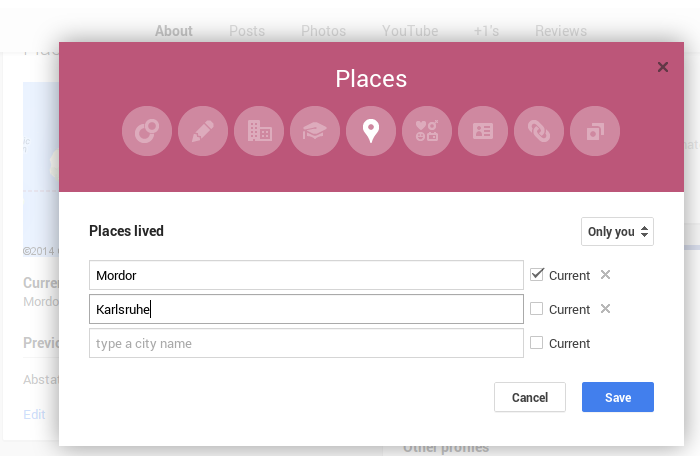
\includegraphics[scale=0.7]{gPlusPlaces.png}

		\begin{enumerate}
			\item Naiver Ansatz -> Geocoding mit Google Maps API V3, nur Indikatoren die geografische Namen enthalten. 
					Prinzipiell einfache Datenbankabfrage mit ein wenig semantik. 
					Keine Jargon Namen wie Big Apple etc.
				\begin{enumerate}
					\item Funktion der GMaps Api V3
					\item Einschränkungen der GMaps Api V3
					\item zurückgelieferte Daten der GMaps Api V3
					\item Kurze Beschreibung wie ich die API genutzt habe
				\end{enumerate}
			\item aktuelle Ansätze
				\begin{enumerate}
					\item{\todo{Ist das grundsätzliche Verfahren, analysieren Inhalt/Indikatoren -> Zuordnen auf geografische Angaben und danach Clustern tatsächlich immer gleich bei allen Arbeiten? kontinuierlich vs diskrete geografische Daten} 
					allgemeiner Ansatz : Geotagged Tweets analysieren (Inhalt/andere Indikatoren usw. ), zuordnen zu geografischen \"Bereichen\" und daraus lernen.}
					\item Verfahren mit Inhaltsanalysen
					\item Verfahren mit Indikatoren einzelne oder mehrere
					\item Welche Verfahren kommen beim mapping auf \todo{geografische Entität definieren} geografische Entitäten zum Einsatz
				\end{enumerate}
		\end{enumerate}

		\subsection{Probleme früherer Ansätze}
			\begin{enumerate}
				\item{Genutzte API's und Indikatoren nur in bestimmten Sprachen verfügbar}
				\item{keine Schätzung für Genauigkeit auf verschiedenen geografischen Hierarchieebenen verfügbar}  
			\end{enumerate}

	
	
	

	


%!TEX root = ../document.tex
\chapter{Lösungsansatz} \label{chp:Loesungsansatz}
	
	\todo{Bezug zum Stand der Technik} 

	Es wird nun ein Verfahren zur Geolokalisierung von Twitter-Nutzern vorgestellt wer den.
	Dabei soll der Standort des Nutzers aus Informationen des Nutzer-Profils bestimmt werden.

	Im ersten Kapitel wird ganz allgemein auf die Geolokalisierung eingegangen.
	Es werden die benötigten Komponenten für eine Geolokalisierung identifiziert und benannt.
	Hierzu wird betrachtet was eine Geolokalisierung leisten muss.
	Danach wird darauf eingegangen wie dies mit Hilfe einer geeigneten Datenbasis umgesetzt werden kann.
	Zum Schluss wird ein generelles Vorgehen zur Geolokalisierung, unter Zuhilfenahme einer Datenbasis, an einem Beispiel erläutert.

	Für die Geolokalisierung eines Twitter-Nutzers werden die Datenwerte des Nutzer-Standortes und der Nutzer-Zeitzone verwendet.
	Diese werden eingehend untersucht.
	Auf Basis dieser Untersuchung wird ein Lernverfahren entwickelt um eine Datenbasis einzulernen.

	Zum Schluss wird ein Verfahren zur Geolokalisierung vorgestellt welches die wahrscheinlichste Georeferenz zu einem gegebenen Twitter-Nutzer ermittelt.
	Dabei wird die eingelernte Datenbasis als Grundlage für die Bestimmung der Georeferenz verwendet.
	
	\newpage
	
	\section{Geolokalisierung} \label{sec:ueberblick} 

		Enthält ein Datensatz Informationen zu einem geografischen Objekt, so können in diesem geografische Indikatoren enthalten sein.
		Durch diese geografischen Indikatoren kann dem Datensatz, und damit dem geografischen Objekt, eine Georeferenz zugewiesen werden. 

		Die Zuordnung einer Georeferenz mit Hilfe von geografischen Indikatoren soll Geolokalisierung genannt werden.  

		In Abbildung \ref{img:geolokalisierung} wird dies dargestellt.
		Im Gegensatz zu Abbildung \ref{img:geogIndi} ist kein direkter Verweis vom geografischen Objekt zu einer Georeferenz vorhanden. 
		Stattdessen wird mit Hilfe der geografischen Indikatoren a und b durch die Geolokalisierung eine Georeferenz zugeordnet.

		\begin{figure}[!ht]
		\begin{center}
		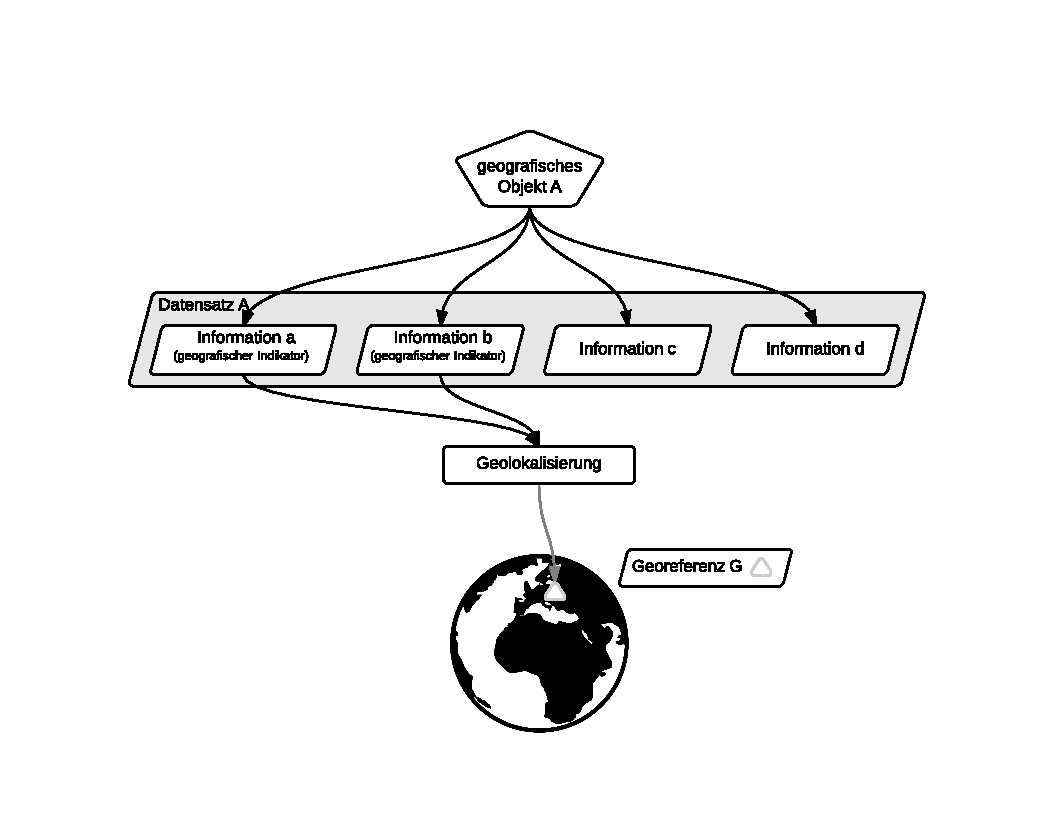
\includegraphics[scale=1.0]{geolokalisierung.pdf}
		\caption{Geografische Hierarchieebenen}
		\label{img:geolokalisierung}
		\end{center}
		\end{figure}	

		Um aus den geografischen Indikatoren eine Georeferenz ableiten zu können soll eine Datenbasis verwendet werden.
		Diese ordnet den geografischen Indikatoren eine Georeferenz zu.
		Die gespeicherte Georeferenz ist bekannt und kann genau bestimmt werden. 
		Das bedeutet: Ein Hinweis auf eine geografische Position wird auf eine konkrete, bekannte geografische Position abgebildet.
		Eine solche Datenbasis soll Georeferenz-Basis genannt werden.  

		Im einfachsten Fall liegt ein geografischer Indikator vor, dem direkt eine Georeferenz zugewiesen werden kann.
		Dies kann Beispielsweise ein eindeutiges Toponym sein.	
		Ein Ortsverzeichnis könnte hier als Georeferenz-Basis verwendet werden.
		Liegt der Datenwert "'Karlsruhe"' vor so würde die Geolokalisierung durch eine Abfrage an die Georeferenz-Basis die Stadt Karlsruhe als Georeferenz zuweisen.

		Wie in Kapitel \ref{sec:ToponymeInGeografischenIndikatoren} bereits erläutert sind Toponyme allerdings nicht immer eindeutig oder bekannt. 
		Die Abfrage an ein Ortsverzeichnis liefert potenziell mehrere Ergebnisse was eine weitere Verarbeitung der Ergebnisse erfordert.
		Ist das Toponym nicht bekannt so kann kein Ergebnis geliefert.

		Des weiteren sind die Datenwerte eines Datensatzes nicht immer direkt zu verwenden.
		Dies kommt ganz darauf an wie die Daten erhoben wurden. 
		Nutzereingaben auf Webseiten können beispielsweise aus einer Liste gewählt, oder in ein Freitext-Feld eingegeben werden.
		Werden die Datenwerte durch eine Liste erhoben liegt eine klar definierte Menge an möglichen Datenwerten vor.
		Haben die Datenwerte in der Liste geografischen Bezug so können ihnen Georeferenzen zugeordnet werden.
		Die so entstandenen Paare aus Datenwert und Georeferenz können in der Georeferenz-Basis abgespeichert werden.

		Soll ein Nutzer in ein Freitext-Feld seinen aktuellen Standort eingeben, und der Datenwert wird direkt übernommen muss dieser vorverarbeitet werden.
		Es ist zwar wahrscheinlich, dass der Nutzer ein Toponym angibt, aber es kann durch die direkte Übernahme der Eingabe zu Problemen kommen.
		Zunächst kann nicht einmal entschieden werden ob der Datenwert überhaupt einen geografischen Indikator darstellt.
		Zudem können in einem Freitext-Feld mehrere geografische Indikatoren auftauchen.
		Diese können widersprüchlich sein oder aber eine geografische Position genauer spezifizieren. 
		Durch die direkte Übernahme des Wertes können alle in Kapitel \ref{sec:ToponymeInGeografischenIndikatoren} aufgeführten Probleme auftreten.
		Dies macht die Zuordnung einer Georeferenz durch eine Ortsverzeichnis schwierig.
		Soll trotzdem mit Hilfe eines Ortsverzeichnisses eine Geolokalisierung durchgeführt werden ist zumindest eine umfangreiche Vor- und Nachverarbeitung nötig.

		In Abbildung \ref{img:geolokalisierungBsp} ist ein Beispiel zur Verwendung einer Georeferenz-Basis dargestellt.
		Der Datenwert "'Karlsruhe"' wird dabei auf eine Georeferenz aufgelöst indem eine Abfrage an die Georeferenz-Basis durchgeführt wird.
		Die zurückgelieferte Georeferenz wird dem Datensatz zugeordnet.

		\begin{figure}[!ht]
		\begin{center}
		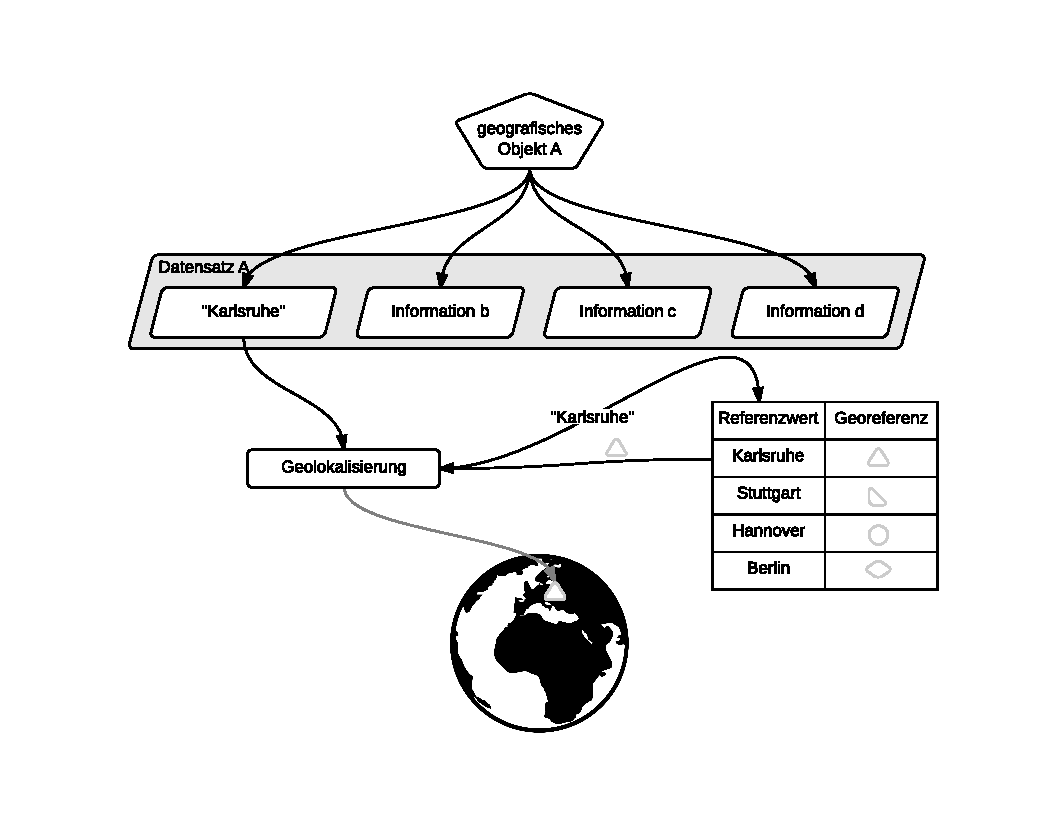
\includegraphics[scale=1.0]{geolokalisierungBsp.pdf}
		\caption{Geolokalisierung mit Referenz-Basis}
		\label{img:geolokalisierungBsp}
		\end{center}
		\end{figure}	

		Im folgenden Kapitel soll eine erste Struktur für eine Georeferenz-Basis vorgestellt werden.
		Es sollen dabei die minimalen Anforderungen an eine solche Datenbasis erfüllt werden.

	\section{Minimale Struktur einer Georeferenz-Basis zur Geolokalisierung} \label{sec:generelleStruktur} 
		
		Nach Abbildung \ref{img:geolokalisierung} wird bei der Geolokalisierung einem oder mehreren geografischen Indikatoren eine Georeferenz zugewiesen.
		In der einfachsten Variante wird lediglich ein einziger geografischer Indikator an die Geolokalisierung übergeben, und genau eine Georeferenz zurückgegeben.
		Die Geolokalisierung muss also zu einem gegebenen geografischen Indikator eine Georeferenz bestimmen können.
		Dies führt zu einer ersten einfachen Struktur für die Georeferenz-Basis.	

		Es wird angenommen der geografische Indikator stellt immer ein eindeutiges Toponym dar.
		Des weiteren sind alle möglichen Toponyme sowie eine zugehörige Georeferenz bekannt. 
		Die Georeferenz liegt als Adresse mit Straße, Hausnummer, Postleitzahl und Ortsname vor.

		Jedem möglichen Toponym soll eine Georeferenz zugeordnet werden können. 
		Die Georeferenz-Basis muss also eine Menge von Toponymen und zugehörigen Georeferenzen beinhalten
		Dieser Aufbau entspricht einer Art Wörterbuch in dem Informationen zu einem gegebenen Referenzwert nachgeschlagen werden können.
		Im vorliegenden Fall kann also zu einem Toponym die entsprechende Georeferenz nachgeschlagen werden.
		Die Referenzwerte stellen dabei mögliche Werte für den geografischen Indikator dar. 
		In Abbildung \ref{tab:simpleStruktur} ist ein Beispiel für eine sehr simple Struktur dargestellt.

		\begin{table}[htpb]
				\caption{Beispiel für eine Georeferenz-Basis} 
				\centering
				\begin{tabular}{|c||c|}
					\hline
					Referenzwert & Georeferenz \\
					\hline\hline
					Zoo-Karlsruhe & Ettlinger Straße 6 - 76137 Karlsruhe \\
					\hline
					ZKM & Lorenzstraße 19 D - 76135 Karlsruhe \\
					\hline
					Elbphilharmonie & Dammtorwall 46 - 20355 Hamburg \\
					\hline
				\end{tabular}
				\label{tab:simpleStruktur} 
		\end{table} 

		Wird eine Abfrage auf die Georeferenz-Basis mit den geografischen Indikatoren "'Zoo-Karlsruhe"', "'ZKM"' oder "'Elbphilharmonie"' durchgeführt, kann nun eine Georeferenz zurückgeliefert werden.
		Diese simple Struktur reicht grundsätzlich aus um eine Geolokalisierung durchführen zu können.
		In dem angeführten Beispiel ist die Menge der möglichen Toponyme sehr begrenzt, aber diese kann beliebig erweitert werden.
		Damit können sehr mächtige Datenbanken erstellt werden.

		Die meisten Ortsverzeichnisse sind nach dieser Struktur aufgebaut, wenngleich sie neben der Georeferenz noch andere Informationen zu einem Toponym liefern.

		Die Form in der die Georeferenz angegeben wird ist abhängig von der Anwendung. 
		Im Beispiel \ref{tab:simpleStruktur} wurden Adressen verwendet. 
		Dazu muss das angegebene Toponym oder die Zeichenkette jedoch eine Adresse besitzen. 
		Ein See in der Wildnis Alaskas wird keine solche Adresse aufweisen.
		Aber auch die geografische Position einer Stadt oder eines Landes kann nicht durch eine Adresse beschrieben werden. 
		Die Form in der die Georeferenz angegeben wird kommt auf den jeweiligen Anwendungsfall an.
		
		\subparagraph{Mögliche Angaben für die Georeferenz}

		\begin{itemize}
		  	 \item geografische Koordinaten
		  	 \item vollständige Adressen
		  	 \item Ländernamen
		  	 \item Städtename
		  	 \item Namen für Verwaltungseinheiten 
		  	 \item Zeitzonen
		  	 \item Straßenname und Kilometerangabe
		  	 \item ...
		  \end{itemize}  

	 	Grundsätzlich sind alle Formen, welche eine direkte oder indirekte Georeferenz darstellen, denkbar.
	 	Die Angabe muss lediglich die gegebenen Anforderungen an die Geolokalisierung erfüllen.

	  	Für den Straßenverkehr ist eine Angabe einer Adresse ausreichend.
		Für Wanderungen in unerschlossenen Gebieten hingegen sind geografische Koordinaten notwendig. 

		Wie in der Liste zu erkennen ist kann die Georeferenz auch als Toponym angegeben werden.
		Wenn nun ein Toponym abgefragt wird, wird als Georeferenz ein Toponym zurückgeliefert.
		Dies macht auf den ersten Blick wenig Sinn.
		Die geografischen Indikatoren sind jedoch vorerst nur Hinweise auf eine Georeferenz.
		Liefert eine Georeferenz-Basis ein Ergebnis zurück, ist der geografische Bezug bestätigt und dem Datensatz kann eine bekannte Georeferenz zugeordnet werden.				
	
	\section{Der Nutzer-Standort und die Nutzer-Zeitzone in Twitter}

		In diesem Kapitel sollen die genutzten Informationen aus dem Twitter-Profil eingehender untersucht werden.
		Dabei werden zum Nutzer-Standort quantitative Daten erhoben um die Eignung des Nutzer-Standorts zur Geolokalisierung zu überprüfen.
		Zusätzlich wird untersucht welche Datenwerte im Nutzer-Standort vorkommen können.

		Bei der Nutzer-Zeitzone wird geprüft ob diese einen geografischen Indikator darstellt. 

		\subsection{Der Nutzer-Standort} \label{subsec:nutzerStandort} 

			Der Nutzer-Standort eines Twitter-Nutzers soll als geografischer Indikator verwendet werden.
			Bei der Eingabe des Nutzer-Standortes wird vom Nutzer abgefragt, wo dieser sich befindet. 
			Die Intention der Abfrage zielt also darauf ab, dass der Nutzer einen Wert eingibt, der auf ein geografisches Objekt verweist. 
			Es ist naheliegend, dass der Nutzer seinen Standort mit Hilfe eines Toponyms angibt.
			Der Nutzer-Standort wird jedoch über ein Freitext-Feld abgefragt und direkt abgespeichert.
			Dieser muss also nicht zwangsweise Werte mit geografischem Bezug enthalten. 

			Sollte es sich bei dem eingegebenen Wert um Toponyme handeln, sind alle in Kapitel \ref{sec:ToponymeInGeografischenIndikatoren} erwähnten Probleme zu erwarten.
			Durch die unkontrollierte Eingabe sind tatsächlich alle möglichen Toponyme denkbar.
			Des weiteren können auch geografische Indikatoren mit mittelbarem geografischen Bezug auftauchen.
			Aber auch Werte die keinen geografischen Bezug aufweisen sind möglich.	

			Zuerst sollen einige allgemeine Kennzahlen zum Nutzer-Standort betrachtet werden.
			Hecht et al. haben in \cite{Hecht2011} den Nutzer-Standort von 10000 Twitter-Nutzern manuell untersucht.
			Um zu bestimmen ob ein Nutzer-Standort geografischen Bezug hat, wurden alle zur Verfügung stehenden Hilfsmittel verwendet.
			Dabei wurden allerdings nur Nutzer aus den USA betrachtet.

			Im Zuge der vorliegenden Arbeit wurde eine eigene Untersuchung von 1000 Nutzer-Standorten verschiedener Nutzer vorgenommen.
			Dazu wurden 1000 Tweets untersucht.
			Die Tweets haben eine zusätzliche Georeferenz in Form von geografischen Koordinaten.
			Diese geben die Position an, von der eine Tweet versendet wurde.
			Für jeden Tweet wurde bestimmt ob der Nutzer-Standort einen geografischen Bezug hat, und darauf basierend eine Georeferenz zugewiesen.
			Als Hilfsmittel hierfür wurden die Ortsverzeichnisse von Google-Map und Geonames.org verwendet.
			Es wurde keinerlei Einschränkung bezüglich der Herkunft des Twitter-Nutzers oder der verwendeten Sprache und des verwendeten Alphabets gemacht.

			Zum Schluss werden die Datenwerte im Nutzer-Standort anhand von Beispielen betrachtet.


			\subsubsection{Geografischer Bezug des Nutzer-Standorts} 
				
				Hecht et al. konnten den Datenwerten in den Nutzer-Standorten in 80\% der Fälle einen geografischen Bezug feststellen.
				In den restlichen 20\% der Fälle konnte im Nutzer-Standort kein geografischer Bezug festgestellt werden. 

				In den eigenen Untersuchungen konnten 76\% der Nutzer-Standorte ein geografischer Bezug nachgewiesen werden. 

				In den restlichen 24\% der Fälle konnte kein geografischer Bezug mit Hilfe der Ortsverzeichnisse nachgewiesen werden. 
				Dies bedeutet nicht, dass grundsätzlich kein geografischer Bezug vorhanden ist. 
				Es konnte lediglich anhand der genutzten Quellen kein geografischer Bezug hergeleitet werden.
				Beispielsweise wurde "'Swag City"' nicht zugewiesen, denn der Spitzname für die Stadt "'Ann Arbor"' war in den Datenbanken nicht hinterlegt. 

				
			\subsubsection{Genauigkeit der geografischen Angaben}
				
				Hecht et al. analysierten ihre Daten darauf wie genau die Nutzer ihren Standort angeben.
				Dabei ist zu beachten, dass die Daten aus den USA stammen und deshalb die Verwaltungseinheiten der USA zugrunde gelegt wurden.
				
				Die Genauigkeiten der Standortangabe nach Hecht et al. sind in \ref{tab:genauigkeitenHecht} angegeben. 

				\begin{table}[htpb]
				\caption{Genauigkeit Standortangabe Hecht et al.} 
				\centering
				\begin{tabular}{|c||c|}
					\hline
					Anteil in \% gerundet & geografische Hierarchieebene \\
					\hline\hline
					64\% & Stadt \\
					\hline
					20\% & Staat \\
					\hline
					ca. 8\% & Intrastate \\
					\hline
					ca. 5 \% & Land \\
					\hline
				\end{tabular}
				\label{tab:genauigkeitenHecht} 
				\end{table} 

				Die restlichen 13\% entfallen auf Interstate Regionen, Nachbarschaften und konkrete Adressen. 
				Interstate Regionen sind Regionen die sich über mehrere Staaten hinwegziehen. 
				Beispiele für Interstate Regionen sind "'Central United States"' oder "'West-Coast"'.
				Nachbarschaften (Neighbourhoods) sind oft Stadtteile wie "'Harlem"' oder "'Bronx"' in New York.

				Bei den eigenen Untersuchungen wurden die geografischen Hierarchieebenen aus Unterkapitel \ref{sub:geografischeHierarchie} zugrunde gelegt.
				Die Genauigkeiten der Standortangabe aus den eigenen Untersuchungen sind in Tabelle \ref{tab:genauigkeitenEigene} angegeben.

				\begin{table}[htpb]
				\caption{Genauigkeit Standortangabe eigene Untersuchungen} 
				\centering
				\begin{tabular}{|c||c|}
					\hline
					Anteil in \% gerundet & geografische Hierarchieebene \\
					\hline\hline
					77\% & Stadt \\
					\hline
					8\% & Verwaltungseinheit erster Ordnung  \\
					\hline
					5\% & Verwaltungseinheit zweiter Ordnung  \\
					\hline
					10 \% & Land \\
					\hline
				\end{tabular}
				\label{tab:genauigkeitenEigene} 
				\end{table} 

				Es ist nicht sicher welche geografische Hierarchieebene im Nutzer-Standort angegeben wird. 

				Die unterschiedlichen Ergebnisse zwischen der eigenen Untersuchung und den Ergebnissen von Hecht et al. können dadurch Zustande kommen, dass in der vorliegenden Arbeit Twitter-Nutzer aus der ganzen Welt untersucht wurden.
				Aber auch der zeitliche Abstand zwischen den beiden Untersuchungen kann dafür verantwortlich sein.  



			\subsubsection{Partieller geografischer Bezug des Datenwertes im Nutzer-Standort} \label{subsec:partiellerGeografischerBezug} 

				In einigen Nutzer-Standorten konnte festgestellt werden, dass nur Teile des eingegebenen Datenwertes geografischen Bezug haben. 
				Es werden oft weitere Informationen angegeben die keinen geografischen Bezug haben. 
				Als Beispiel hierfür sollen "'11th Dimension | California"' und "'between here and there - Miami"' betrachtet werden.
				Im ersten Fall kann für "'California"' ein unmittelbarer geografischer Bezug festgestellt werden.
				"'11th Dimension"' hat hier offensichtlich keinen geografischen Bezug.
				Im zweiten Fall ist die Aussage "'between here and there"' ohne geografischen Bezug.
				"'Miami"' kann jedoch als Bezug zur Stadt Miami in Florida gebracht werden.
				
				Es können also auch nur Teile des Nutzer-Standorts für eine Geolokalisierung von Nutzen sein.

			\subsubsection*{Widersprüchliche Datenwerte im Nutzer-Standort} \label{subsec:wiederspruechlicheBezuege} 

				Es existieren auch Datenwerte in denen mehrere widersprüchliche Angaben gemacht werden.
				Dies bedeutet es werden zwei oder mehr Datenwerte mit geografischem Bezug angegeben, die auf unterschiedliche geografische Objekte verweisen.

				Auch hier sollen einige Beispiele genannt werden:

				\begin{itemize}
					\item Bolton\textbackslash/Leigh
					\item Liverpool\textbackslash/London
					\item  Balikesir \textbackslash/ Izmir	
				\end{itemize}							
					
				In diesen Beispielen sind jeweils zwei Städte angegeben.
				Bolton und Leigh liegen 14km auseinander.
				Liverpool und London trennen ca. 350km.
				Balikesir und Izmir ca. 180km.

				Es kann nun spekuliert werden wieso der Nutzer zwei Städte angibt.
				Ist er in einer Stadt aufgewachsen und lebt momentan in der anderen?
				Pendelt er zwischen den Städten um zu arbeiten?

				Wie dem auch sei, es kann nicht eindeutig entschieden werden in welcher Stadt sich der Nutzer aufhält.

			\subsubsection*{Geografische Hierarchien im Nutzer-Standort}

				Es ist auch möglich, dass im Nutzer-Standort teile einer geografischen Hierarchie angegeben sind.
				Beispielsweise die Angabe einer Stadt in Kombination mit einem Land.
				
				In den USA wird beispielsweise oft die Stadt und der zugehörige Bundesstaat angegeben.
				In Brasilien hingegen wird oft ein Bundesstaat und das Land angegeben.
				Hier einige Beispiele:

				\begin{itemize}
					\item Los Angeles, California
					\item Mato Grosso, Brazil
					\item Bronx, New York	
				\end{itemize}		

				Im ersten Beispiel handelt es sich um die Stadt Los Angeles und den US-Bundesstaat Kaliforniern.
				Im zweiten Beispiel wird zuerst ein brasilianischer Bundesstaat angegeben und danach das Land.
				Im dritten Beispiel wird ein Stadtteil von New York angegeben und dann die Stadt oder der US-Bundesstaat. 
				Da der US-Bundesstaat denselben Namen hat wie die Stadt, und beide in einer Hierarchiebeziehung mit Bronx stehen, kann hier nicht unterschieden werden was gemeint ist.
				
			\subsubsection{Domänenspezifische Toponyme im Nutzer-Standort} 

				In sozialen Netzwerken können sich eigene Begriffe und Formulierungen etablieren. 
				Diese sind im allgemeinen nicht bekannt.

				Im Twitter-Umfeld haben sich in den letzten Jahren einige spezielle Begriffe und Formulierungen zur Verwendung in Tweet-Texten etabliert. 
				Das im Twitter-Umfeld auch spezielle Toponyme verwendet werden, kann nicht gänzlich ausgeschlossen werden. 

				Ein Beispiel hierfür ist "'Bieberville"', welches in den untersuchten Daten von Hecht et al. öfter vorkommt.
				"'Bieberville"' wird abgeleitet von dem Pop-Star Justin Bieber.	
				Twitter wird oft als "'Bieberville"' bezeichnet.
				Da der Pop-Star in Twitter sehr aktiv ist und deshalb viele seiner Fans auch in Twitter aktiv sind hat sich dieser Name etabliert.
				Unter diesem Gesichtspunkt hätte "'Bieberville"' keinen geografischen Bezug.
				Sucht man allerdings im Internet nach "'Bieberville"' stößt man auf einen Imbiss in Groß-Bieberau.
				"'Bieberville"' kann also durchaus einen geografischen Bezug haben, wenngleich es im Twitter-Umfeld nicht als solcher benutzt wird. 
				Ein Nutzer-Standort der in einem Land kein Toponym darstellt, kann in einem anderen durchaus ein Toponym sein.
				Ist in einem Ortsverzeichnis beispielsweise "'Bierberville"' als Bezeichnung für den Imbiss in Groß-Bieberau hinterlegt, würde dieser als Georeferenz zugeordnet werden, was im Umfeld von Twitter in einem Großteil der Fälle falsch wäre.

				Solche Begriffe und Formulierungen können nur sehr schlecht mit einem Ortsverzeichnis zu Georeferenzen zugeordnet werden. 

		\subsection{Die Nutzer-Zeitzone}

			In Kapitel \ref{sec:ToponymeInGeografischenIndikatoren} wurde auf die Probleme bei der Verwendung von Toponymen als geografische Indikatoren eingegangen.
			Dabei wurde die Doppel- und Mehrdeutigkeit von Toponymen betrachtet.
			Bei der Verwendung des Nutzer-Standortes als geografischen Indikator kann dieses Problem auch auftauchen. 

			Um diesem Problem zu begegnen soll die Nutzer-Zeitzone als weiterer geografischer Indikator hinzugezogen werden.
			Zunächst sollen die generellen Eigenschaften der Nutzer-Zeitzone erläutert werden bevor erklärt wird wie die Nutzer-Zeitzone das Problem der Mehrdeutigkeit von Toponymen beheben kann.

			\subsubsection{Eigenschaften der Nutzer-Zeitzone}

				Die Nutzer-Zeitzone stellt einen geografischen Indikator dar.
				Sie beschreibt eine eindeutige geografische Region auf dem Globus und somit hat direkten geografischen Bezug.
				Dabei entsprechen die Grenzen der Region nicht unbedingt den Landesgrenzen oder den Grenzen sonstiger Verwaltungseinheiten. 
				In Abbildung \ref{img:timezones} sind die Zeitzonen der Erde dargestellt.

				\begin{figure}[!ht]
					\begin{center}
						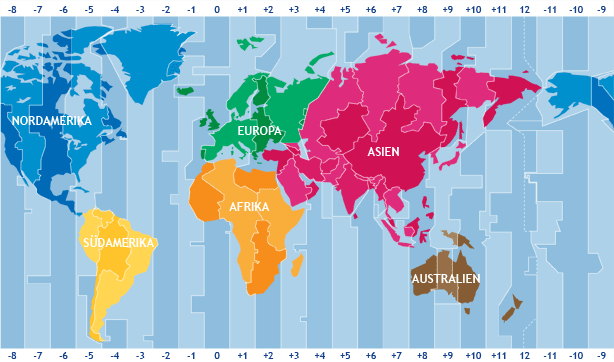
\includegraphics[scale=0.5]{zeitzonen_weltkarte.jpg}
						\caption{Zeitzonen der Erde.}
						\label{img:timezones}
					\end{center}
				\end{figure}	
				%Quelle: http://www.zeitzonen.de/images/frontend/mod\_tz\_map/zeitzonen\_weltkarte.gif

				Die Nutzer-Zeitzone kann in Twitter über eine Liste gewählt werden.
				Der Wert der Nutzer-Zeitzone stellt deshalb garantiert eine Zeitzone dar.
				Es ist dem Nutzer nicht möglich einen Wert einzugeben der nicht einer Zeitzone entspricht.

				In Abbildung \ref{img:usTimezones} wurden Tweets anhand ihres Längen- und Breitengrades platziert.
				Jeder Punkt in der Abbildung entspricht einem Tweet.
				Es wurden nur Tweets aus den USA ausgewählt.
				Anhand der Nutzer-Zeitzone wurde jedem Tweet eine Farbe zugeordnet.
				In Tabelle \ref{tab:timezoneColors} sind die Farbzuordnungen aufgelistet. 

				\begin{table}[h]
				\centering
				\caption{Zeitzonen Farben}
				\label{tab:timezoneColors}
					\begin{tabular}{|l|l|}
						\hline
						Zeitzone      & Farbe     \\ \hline \hline
						Pacific Time  & Rot       \\ \hline
						Eastern Time  & Grün/Gelb \\ \hline
						Central Time  & Blau      \\ \hline
						Mountain Time & Pink      \\ \hline
					\end{tabular}
				\end{table}

				 \begin{figure}[!ht]
					\begin{center}
						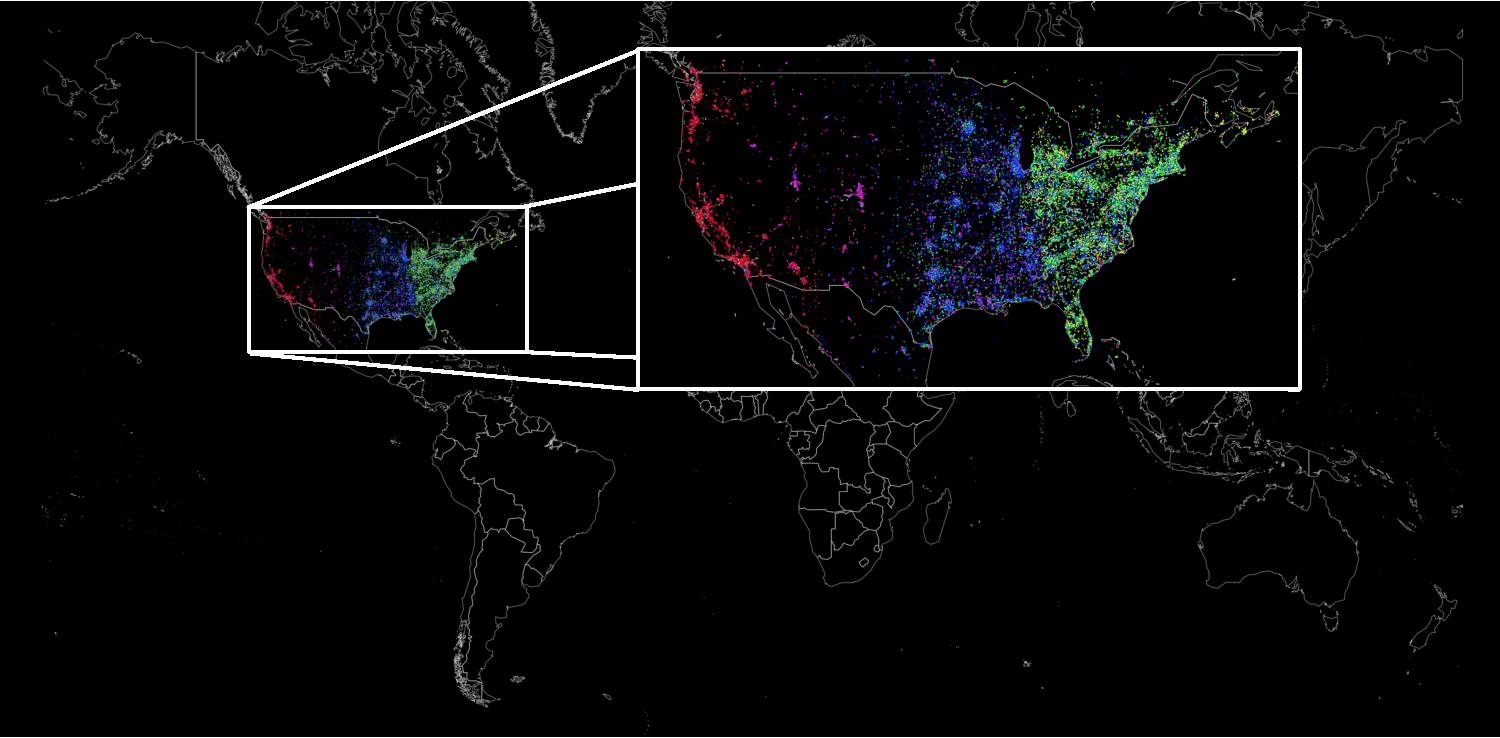
\includegraphics[scale=0.5]{usTimezones.pdf}
						\caption{Tweets, abhängig der Zeitzone eingefärbt}
						\label{img:usTimezones}
					\end{center}
				\end{figure}	

				 Die Zeitzonen sind an den Farben gut zu erkennen. 
				 Lediglich die dünn besiedelte Region der Mountain Time kann nur an einigen Ballungszentren erkannt werden. 
				 Grundsätzlich scheint der Großteil der Angaben aber korrekt zu sein.

			\subsubsection{Auflösen von Doppeldeutigkeiten}

				Ist ein Toponym Doppel- oder Mehrdeutig kann nicht entschieden werden welches geografische Objekt zugeordnet werden soll.
				Liegen die beiden geografischen Objekte allerdings in zwei unterschiedlichen Zeitzonen und der Nutzer hat eine Nutzer-Zeitzone angegeben kann die Doppeldeutigkeit aufgelöst werden.
				Es muss lediglich die Nutzer-Zeitzone betrachtet werden.
				Somit kann dem Nutzer eine korrekte Georeferenz zugewiesen werden.
				Voraussetzung hierfür ist natürlich, dass die geografischen Objekte in zwei unterschiedlichen Zeitzonen liegen und die Nutzer-Zeitzone angegegeben ist.

		\subsection{Fazit} 

			In ca. 80\% der Fälle kann der Nutzer-Standort tatsächlich einen Hinweis auf eine Georeferenz liefern.
			Die Eingaben sind allerdings nicht standardisiert und können somit nicht ohne Vorverarbeitung verwendet werden.
			Wie oben dargestellt kann der Nutzer-Standort nur partiellen geografischen Bezug haben.
			Es können mehrere Informationen verschiedener geografischer Hierarchieebenen im Datenwert auftauchen. 
			Und die Datenwerte im Nutzer-Standort können keinerlei geografischen Bezug aufweisen.
			Dies macht es grundsätzlich schwierig die Datenwerte im Nutzer-Standort direkt als geografischen Indikator zu verwenden.
			
			Ist ein geografischer Bezug des Nutzer-Standortes nachzuweisen, handelt es sich bei dem Eintrag in den meisten Fällen um ein Toponym.
			Bei der durchgeführten Untersuchung wurden nur Ortsverzeichnisse zur Bestimmung eines geografischen Bezugs verwendet.
			In Ortsverzeichnissen sind nur Toponyme hinterlegt es kann deshalb davon ausgegangen werden, dass ca. 76\% der Nutzer-Standorte auf Toponyme zurückzuführen sind.

			Widersprüchliche Angaben, geografische Hierarchien und partieller geografischer Bezug können bei der Geolokalisierung zu Problemen führen.
			Diese entstehen meist dadurch, dass der Datenwert nicht nur eine konkrete, sondern mehrere Angaben beinhaltet.
			
			Um den Problemen zu begegnen sollen die Datenwerte im Nutzer-Standort einer Vorverarbeitung unterzogen werden. 
			Dadurch sollen möglichst viele einzelne Informationen aus dem Nutzer-Standort extrahiert werden.

			Es können Beispielsweise Datenwerte mit geografischem Bezug von Datenwerten ohne geografischen Bezug getrennt untersucht werden.

			Sollten Mehrdeutigkeiten im Nutzer-Standort auftauchen können diese teilweise durch die Hinzunahme der Nutzer-Zeitzone aufgelöst werden.

	\section{Verfahren zum einlernen geografischer Indikatoren am Beispiel von Twitter} \label{sec:einlernen}  

		Die Probleme bei der Nutzung von Ortsverzeichnissen sind meist auf deren Unvollständigkeit zurückzuführen. 
		Um dies zu umgehen soll die Georeferenz-Basis automatisch eingelernt werden. 

		Der Vorteil besteht darin, dass eine domänenspezifische Georeferenz-Basis geschaffen wird.
		Diese kann potenziell mehr geografische Indikatoren zuordnen als ein normales Ortsverzeichnis.
		Denn es können dadurch domänenspezifische Eigenheiten bei der Verwendung von Toponymen berücksichtigt werden. 
		Auch domäneninterne Begriffe sollen hierdurch gelernt werden können.

		Im ersten Unterkapitel soll der Ablauf und die nötigen Daten zur Umsetzung eines solchen Lernverfahrens erläutert werden.

		Danach wird auf die Vorverarbeitung des Nutzer-Standortes eingegangen.
		Es werden basierend auf den erzeugten Referenzwerten und den zugeordneten Georeferenzen absolute Häufigkeiten bestimmt.
		Des weiteren wird die in Abschnitt \ref{sec:generelleStruktur} vorgestellte Struktur der Georeferenz-Basis angepasst und erweitert.
		Dabei wird am grundsätzlichen Prinzip nichts geändert, es wird nach wie vor einem Referenzwert eine Georeferenz zugewiesen. 

		\subsection{Allgemeiner Ablauf des Lernverfahrens}

			Die eingelernte Georeferenz-Basis soll es ermöglichen durch die Datenwerte im Nutzer-Standort und der Nutzer-Zeitzone eine Georeferenz zu bestimmen.
			Nach der Struktur aus Kapitel \ref{sec:generelleStruktur} besteht eine Georeferenz-Basis zumindest aus Referenzwerten und einer zugeordneten Georeferenz.
			Die Referenzwerte sollen aus dem Nutzer-Standort und der Nutzer-Zeitzone erzeugt werden.
			Um eine Georeferenz zuordnen zu können muss zu jedem Tupel aus Nutzer-Standort und Nutzer-Zeitzone eine Georeferenz vorliegen.
			Als Basis für das Lernverfahren werden die Tweet-Lerndaten genutzt.
			Jeder Tweet enthält dabei neben dem Nutzer-Standort und der Nutzer-Zeitzone eine Georeferenz in Form von Längen- und Breitengrad. 
			Die Tweets sollen mit Hilfe des Längen- und Breitengrades der nächstgelegenen Stadt zugeordnet werden. 
			Dadurch kann jedem Referenzwert in der Georeferenz-Basis später eine Stadt als Georeferenz zugeordnet werden.
			Es entstehen somit Tupel aus einem Referenzwert und einer zugehörigen Georeferenz.
			Diese sollen in der Georeferenz-Basis gespeichert werden.

			Zusätzlich soll ein neues Feld in der Georeferenz-Basis eingeführt werden.
			Dieses soll angeben, wie oft die Kombination aus einem Referenzwert und einer Stadt vorgekommen ist. 
			Das Feld gibt also die absolute Häufigkeit der Vorkommen an.
			Nachdem die Georeferenz-Basis eingelernt ist liegen somit für jeden Referenzwert eine Georeferenz und die absolute Häufigkeit vor.
			Basierend darauf können dann die relativen Häufigkeiten für jedes paar aus Referenzwert und Stadt berechnet werden.
			Bei der Geolokalisierung werden diese Werte genutzt um die wahrscheinlichste Georeferenz für einen gegebenen Nutzer-Standort und Nutzer-Zeitzone zu bestimmen.

			In Abbildung \ref{img:EinlernenAllg} ist das Verfahren zum einlernen einer Georeferenz-Basis an einem Beispiel dargestellt.

			\begin{figure}[!ht]
					\begin{center}
						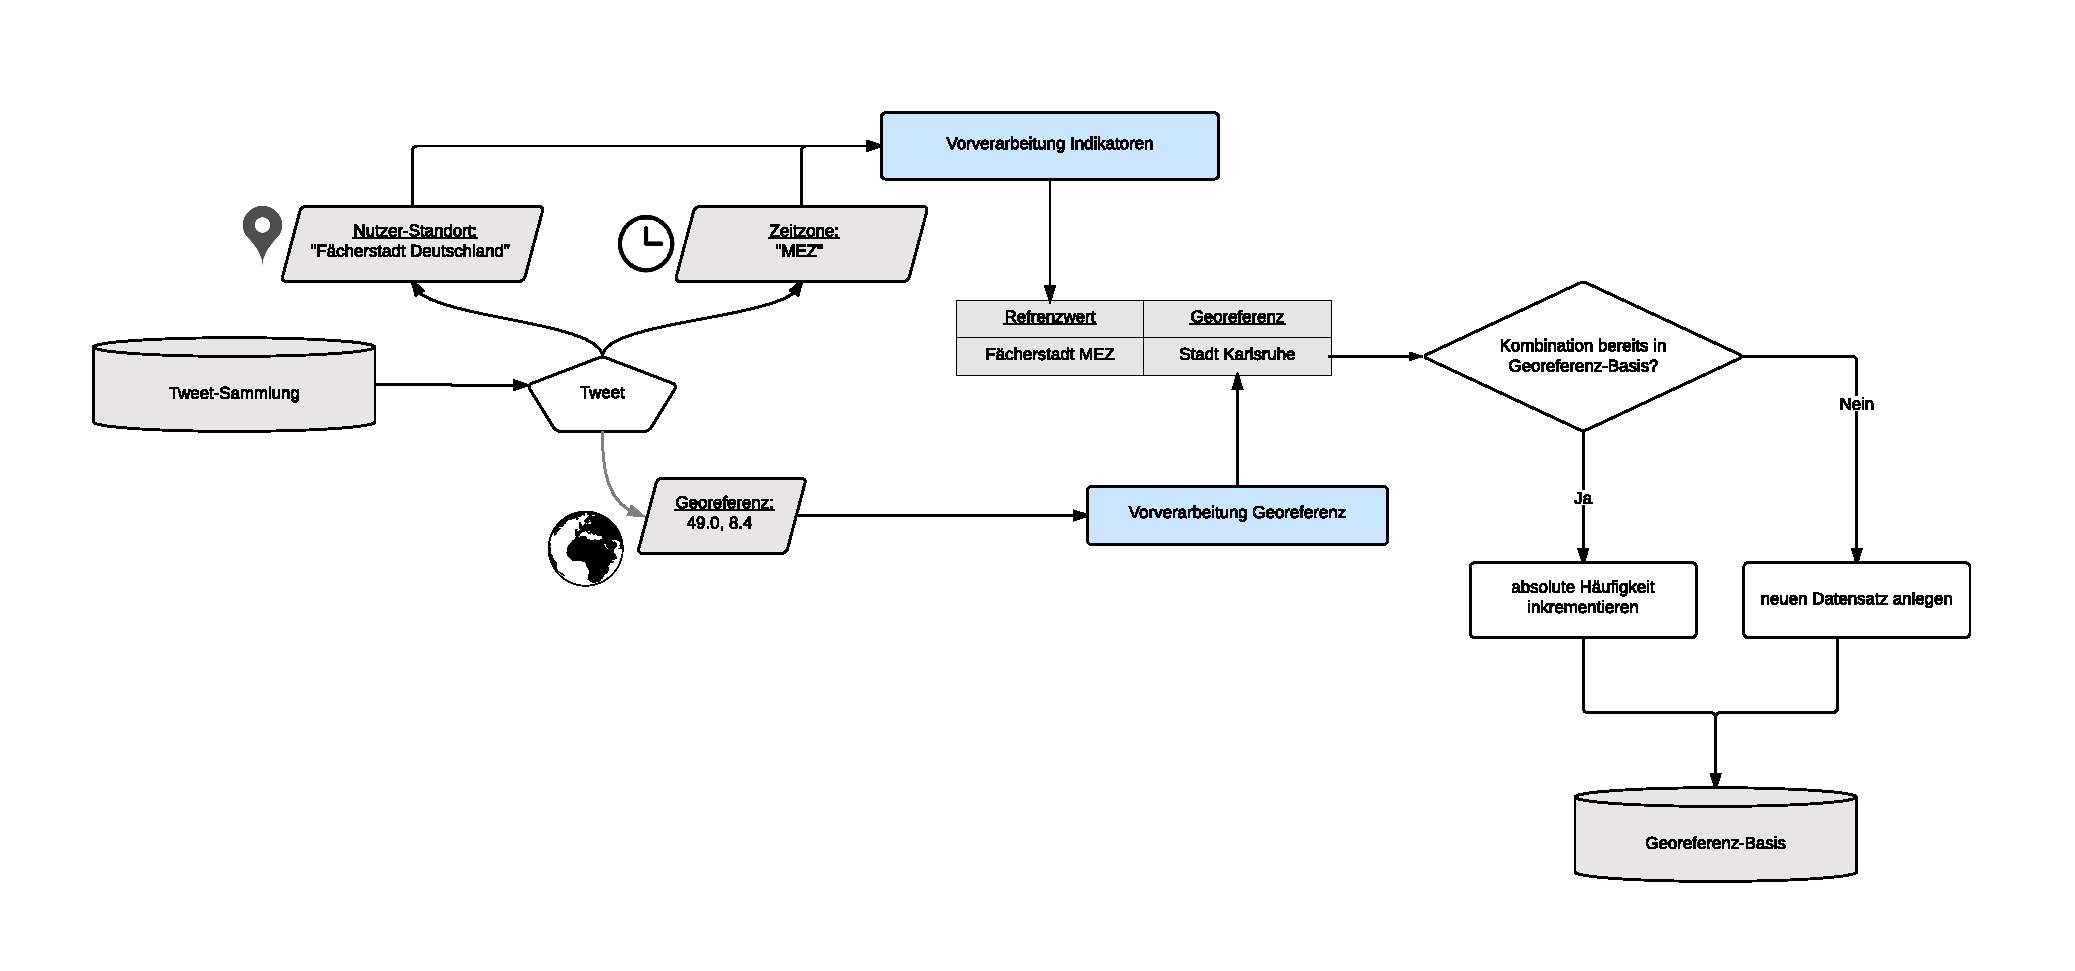
\includegraphics[scale=0.5]{einlernenAllg.pdf}
						\caption{Verfahren zum einlernen einer Georeferenz-Basis}
						\label{img:EinlernenAllg}
					\end{center}
			\end{figure}	

			In den nächsten Unterkapiteln sollen nun die einzelnen Schritte des Verfahrens genauer betrachtet werden. 
			Zudem wird die Erweiterung der Datenbasis erläutert.

		\subsection{Vorverarbeitung des Nutzer-Standortes und der Nutzer-Zeitzone} \label{subsec:VorverarbeitungStandortZeitzone} 
			
			Es ist zunächst nötig die genutzten geografischen Indikatoren einer Vorverarbeitung zu unterziehen. 
			Ziel ist es aus dem Nutzer-Standort möglichst viele Informationen zu extrahieren und etwaige Probleme zu beseitigen.
			In der folgenden Liste sind einige Nutzer-Standorte angegeben. 
			Anhand dieser Liste sollen die Vorverarbeitungsschritte demonstriert werden.

			\begin{multicols}{2}
			\begin{enumerate}
				\item Bélem-PA
				\item West Sussex, England
				\item South Florida
				\item Pitmedden,  Scotland, UK
				\item Mato Grosso \& Rio de Janeiro
				\item -****-
				\item USA \textbackslash/ Los Angeles
				\item Nottingham\textbackslash/London
				\item Los Angeles, USA
				\item I $\heartsuit$ New York 
				\item $\dagger$\textasciitilde Los Angeles\textasciitilde$\dagger$
				\item earth-sea
				\item In front of the computer
				\item 11th Dimension | California
				\item York
				\item York
			\end{enumerate}
			\end{multicols}
				
			\subsubsection{Eliminierung von Sonder- und Satzzeichen} 

				Es werden oft Sonder- und Satzzeichen im Nutzer-Standort verwendet. 
				Beispielsweise als Trenner zwischen Toponymen unterschiedlicher geografischer Hierarchieebenen.
				Beispiele hierfür sind "'West Sussex, England"', "'USA \textbackslash/ Los Angeles"' oder "'Bélem-PA"'.
				Das Trennzeichen wird dabei nicht einheitlich verwendet.  
				Es kann deshalb nicht entschieden werden ob ein Satzzeichen als Trenner zweier Hierarchieebenen genutzt wird oder nicht.
				Bei "'USA \textbackslash/ Los Angeles"' wird \textbackslash/ als Trenner für Hierarchieebenen verwendet.
				Bei "'Nottingham\textbackslash/London"' hingegen werden zwei Städte angegeben.
				Es ist also insbesondere nicht klar welcher Zusammenhang zwischen den Datenwerten, die durch ein Sonder- oder Satzzeichen getrennt sind, besteht. 

				Bei "'I $\heartsuit$ New York "' werden Sonderzeichen zum ausdrücken von Emotionen genutzt.
				In "'$\dagger$\textasciitilde Los Angeles\textasciitilde$\dagger$"' werden Sonderzeichen als Dekoration genutzt.
				Einige Nutzer-Standorte bestehen ausschließlich aus Sonder- und Satzzeichen.
				
				Grundsätzlich ist es aufgrund schwierig zu entscheiden ob Satz- und Sonderzeichen einen Mehrwert bieten um einen Nutzer-Stadort genauer zu bestimmen.
				Dies ist immer dann der Fall, wenn die Sonder- und Satzzeichen Bestandteil eines Toponyms sind. 
				Es gibt tatsächlich Fälle in denen Sonder- oder Satzzeichen Bestandteil eines Toponyms sind.
				Ein Beispiel hierfür wäre "'3. Arrondisement Paris"'.
				Das weggelassen des Punktes hätte allerdings keinen Einfluss auf die gelieferte Information.

				In den oben genannten Fällen bringen Sonder- und Satzzeichen keine zusätzlichen Informationen.
				Es sollen deshalb in einem ersten Vorverarbeitungsschritt alle Sonder- und Satzzeichen entfernt werden. 

				Liste nach dem entfernen von Sonder- und Satzzeichen:

				\begin{multicols}{2}
					\begin{enumerate}
						\item Bélem PA
						\item West Sussex England
						\item South Florida
						\item Pitmedden Scotland UK
						\item Mato Grosso Rio de Janeiro
						\item 
						\item USA Los Angeles
						\item Nottingham London
						\item Los Angeles USA
						\item I New York 
						\item Los Angeles
						\item earth sea
						\item In front of the computer
						\item 11th Dimension California
						\item York
						\item York
					\end{enumerate}
				\end{multicols}

				Der Wert 6 existiert nun nicht mehr, der Wert ist leer und wird somit nicht weiter betrachtet.

				Unnötige Sonder- und Satzzeichen wurden entfernt und die entstandenen Werte können nun einfacher weiterverarbeitet werden.

			\subsubsection{Zusammenfassen von Toponymen}

				Oft bestehen Toponyme aus zwei oder mehr Worten.
				Diese sollen mit Hilfe eines Ortsverzeichnisses zusammengefasst werden. 
				Dies kann selbstverständlich nur für bekannte Toponyme durchgeführt werden.
				
				"'Los"' und "'Angeles"' bilden gemeinsam "'Los Angeles"' und sollen in der weiteren Verarbeitung gemeinsam betrachtet werden. 
				Dies soll zunächst mit einem + Zeichen gekennzeichnet werden.

				Daraus resultiert:

				\begin{multicols}{2}
					\begin{enumerate}
						\item Bélem PA
						\item West+Sussex England
						\item South Florida
						\item Pitmedden Scotland UK
						\item Mato+Grosso Rio+de+Janeiro
						\item USA Los+Angeles
						\item Nottingham London
						\item Los+Angeles USA
						\item I New+York 
						\item Los+Angeles
						\item earth sea
						\item In front of the computer
						\item 11th Dimension California
						\item York
						\item York
					\end{enumerate}
				\end{multicols}

				In diesem Schritt wird insbesondere keine Geolokalisierung vorgenommen. 
				Er dient dazu möglichst früh vorhandenes Wissen über Toponyme einzubeziehen und somit eine unnötige Fragmentierung zu vermeiden.
				Im wesentlichen sollen die Werte hiermit für die nächsten Verarbeitungsschritte vorbereitet werden.

			\subsubsection{Alphanumerische Sortierung}

				In diesem Schritt sollen die Werte alphanumerisch sortiert werden. 

				Nach der Sortierung liegt folgende Tabelle vor:

				\begin{multicols}{2}
					\begin{enumerate}
						\item Bélem PA
						\item England West+Sussex
						\item Florida South
						\item Pitmedden Scotland UK
						\item Mato+Grosso Rio+de+Janeiro
						\item Los+Angeles USA
						\item London Nottingham
						\item Los+Angeles USA
						\item I New+York 
						\item Los+Angeles
						\item earth sea
						\item computer front In of the 
						\item 11th California Dimension 
						\item York
						\item York
					\end{enumerate}
				\end{multicols}

				Die Werte 6 und 8 sind nun gleich. 
				Durch die Sortierung werden Werte mit gleichem Inhalt aber unterschiedlicher Reihenfolge angeglichen.
				Durch das zusammenfassen der Toponyme im vorherigen Schritt werden bekannte Toponyme nicht getrennt.

				Dieser Schritt stellt allerdings einen Kompromiss dar.
				Es werden zwar Werte mit gleichem Inhalt und unterschiedlicher Reihenfolge angeglichen.
				Aber es werden auch potenzielle Toponyme, die aus mehreren Teilen bestehen, auseinandergezogen.
				Aus "'Motor City Michigan USA"' würde "'City Michigan Motor USA"' entstehen.
				Der Zusammenhang zwischen Motor und City wäre nicht mehr vorhanden und könnte auch nicht wiedergewonnen werden.

			\subsubsection{Erzeugung von N-Grammen}

				Es sollen nun N-Gramme bis zum Grad 3 erzeugt werden. 
				Dieses Vorgehen löst gleich mehrere Probleme.

				Zum ersten können sowohl geografische Indikatoren als auch Werte die kein geografischen Indikator darstellen in den Nutzer-Standorten vorhanden sein.
				Durch die Erzeugung von N-Grammen können diese getrennt voneinander betrachtet werden.
				Es löst das Problem des partiellen geografischen Bezugs des Nutzer-Standortes aus \ref{subsec:partiellerGeografischerBezug} in der Hinsicht, dass die Werte für die weitere Verarbeitung getrennt betrachtet werden können.

				Zum zweiten können in einem Nutzer-Standort mehrere geografische Indikatoren enthalten sein.  
				Der Wert "'Pitmedden Scotland UK"' enthält mit "'UK"' das Land, mit "'Scottland"' den Landesteil und mit "'Pitemedden"' eine Stadt. 
				Mit dem Längen- und Breitengrad aus dem zugehörigen Tweet kann nun allen drei Werten eine Georeferenz zugeordnet werden.

				Aber auch zwei verschiedene Städte wie "'Nottingham\textbackslash/London"' können in einem Wert vorkommen.
				Diese werden zu "'Nottingham\textbackslash/London"', "'Nottingham"' und "'London"'.
				Wird hier wiederum beiden Werten die geografische Koordinate zugeordnet können drei Fälle auftreten.
				Erstens: Der Nutzer war in keiner der beiden Städte als er den Tweet abgesetzt hat. 
				Damit sind beide Zuordnungen unbrauchbar.
				Zweitens: Er war in einer der beiden Städte, dann ist zumindest einer der entstandenen Datensätze brauchbar.
				Dies löst das Problem aus \ref{subsec:wiederspruechlicheBezuege} in der Hinsicht, dass die Werte für die weitere Verarbeitung getrennt betrachtet werden können.

				Besteht allerdings eine Beziehung der Werte zueinander, kann diese durch Bi- und Trigramme abgebildet werden.
				Aus "'Pitmedden Scotland UK"' wird "'Pitmedden Scotland"', "'Scotland UK"' und "'Pitmedden Scotland UK"' erzeugt.

				Dieser Schritt soll nur an einigen ausgewählten Beispielen aus der Liste erfolgen.
				Die Bestandteile der N-Gramme werden zur Verdeutlichung mit \textless \textgreater gekennzeichnet in späteren Beispielen wird dies weggelassen, da durch das zusammenfassen von Werten mit einem plus klar ist welches die Elemente des NGramms darstellen

				\begin{multicols}{2}
					\begin{enumerate}
						\item \textless England\textgreater   \textless West+Sussex\textgreater  
						\item \textless England\textgreater  
						\item \textless West+Sussex\textgreater  
						\item \textless Mato+Grosso\textgreater   \textless Rio+de+Janeiro\textgreater  
						\item \textless Rio+de+Janeiro\textgreater  
						\item \textless Mato+Grosso\textgreater  
						\item \textless 11th\textgreater   \textless California\textgreater   \textless Dimension\textgreater   
						\item \textless 11th\textgreater   \textless California\textgreater  
						\item \textless California\textgreater   \textless Dimension\textgreater   
						\item \textless 11th\textgreater  
						\item \textless California\textgreater  
						\item \textless Dimension\textgreater   
						\item \textless York\textgreater  
						\item \textless York\textgreater  
					\end{enumerate}
				\end{multicols}
				Der Wert 7 ist ein Trigramm.
				Bei den Werten 1,4,8 und 9 handelt es sich um Bigramme. 
				Die Werte von 2,3,5,6,10,11 und 12 sind Unigramme.				

				In diesem Schritt werden aus dem Nutzer-Standort mehrere potenzielle geografische Indikatoren erzeugt die als Referenzwerte genutzt werden können.
				Bevor diese als Referenzwerte genutzt werden soll aber noch die Nutzer-Zeitzone einbezogen werden.

			\subsubsection{Hinzufügen der Nutzer-Zeitzone}

				Die Zeitzone stellt eine begrenzte Anzahl an Werten dar.
				Diese werden vom Nutzer nicht frei eingegeben. 
				Es wird hier hier deshalb keine weitere Vorverarbeitung vorgenommen.

				An die Referenzwerte, die aus dem Nutzer-Standort erzeugt wurden soll nun die Zeitzone angehängt werden.
				Jeder Referenzwert soll einmal mit und einmal ohne Zeitzone existieren. 
				Damit wird garantiert, dass eingelernte Referenzwerte die eine falsche Zeitzone aufweisen, trotzdem berücksichtigt werden können. 
				Beispielsweise ist die Nutzer-Zeitzone "'Pacific Time (US \& Canada)"' für den Nutzer-Standort "'Jakarta"' nicht korrekt.
				Aus dieser Kombination würden die Referenzwerte "'Jakarta Pacific Time (US \& Canada)"' und "'Jakarta"' entstehen. 
				Bei einer Abfrage von "'Jakarta"' kann dann trotzdem der Referenzwert "'Jakarta"' genutzt werden. 
				Würde allerdings nur die Kombination "'Jakarta Pacific Time (US \& Canada)"' als Referenzwert existieren würde keine Georeferenz zurückgeliefert werden können.

				Die Elemente der Zeitzonen werden wiederum mit einem Plus zusammengefasst um deutlich zu machen, dass es sich um ein Element eines NGramms handelt.
				Um die Nutzer-Zeitzone von den aus dem Nutzer-Standort generierten Elementen unterscheiden zu können, wird die Nutzer-Zeitzone kursiv geschrieben.
				Auch hier wird die Liste weiter eingeschränkt und es werden lediglich noch zwei Beispiele betrachtet.
				\begin{multicols}{2}
					\begin{enumerate}
						\item England West+Sussex
						\item  England  
						\item  West+Sussex  
						\item  England    West+Sussex   \textit{London}
						\item  England   \textit{London}
						\item  West+Sussex   \textit{London}
						\item  11th    California    Dimension    
						\item  11th    California  
						\item  California    Dimension   
						\item  11th  
						\item  California  
						\item  Dimension   
						\item  11th  California    Dimension   \textit{Pacific+Time+US+Canada}
						\item  11th    California   \textit{Pacific+Time+US+Canada}
						\item  California    Dimension   \textit{Pacific+Time+US+Canada}
						\item  11th   \textit{Pacific+Time+US+Canada}
						\item  California   \textit{Pacific+Time+US+Canada}
						\item  Dimension   \textit{Pacific+Time+US+Canada}
						\item York
						\item  York   \textit{London}
						\item York
						\item  York   \textit{Eastern+Time}
					\end{enumerate}	
				\end{multicols}
				Mit Hilfe der Zeitzone können nun auch die beiden letzten Einträge unterschieden werden. 
				Zum einen "'York"' in England zum anderen "'York"' in den USA. 
				Dies löst das Problem der Mehrdeutgkeiten von Toponymen. 
				Mit Hilfe der zusätzlichen Zeitzone können geografische Objekte, zumindest wenn sie in zwei verschiedenen Zeitzonen liegen, unterschieden werden.

			\subsubsection{Fazit} 

				Nach der Vorverarbeitung liegen eine Menge von potenziellen geografischen Indikatoren mit zugehörigen geografischen Koordinaten vor.
				Bei der Vorverarbeitung wurden einige Probleme des Nutzer-Standortes beseitigt.
				Insbesondere können Datenwerte separat voneinander betrachtet werden.

				Die so erzeugten potenziellen geografischen Indikatoren können nun in der Georeferenz-Basis als Referenzwerte gespeichert werden.
				Mit der so erzeugten Georeferenz-Basis ist es grundsätzlich möglich eine Geolokalisierung durchzuführen. 
				Allerdings wird jedem potenziellen geografischen Indikator eine Georeferenz zugeordnet.
				Das ist grundsätzlich problematisch, da Referenzwerten die keinen geografischen Bezug aufweisen eine Georeferenz zugeordnet wird. 
				Dies kann bei der Geolokalisierung zu Fehlern führen.
				Ein Referenzwert mit geografischem Bezug wird gleich behandelt wie ein Referenzwert ohne geografischen Bezug.
				Es sollte entschieden werden können ob der Referenzwert einen geografischen Bezug hat oder nicht.
				Bisher existiert noch kein Hinweis auf den geografischen Bezug.
				Es existiert lediglich eine Datenbasis die Referenzwerten eine Georeferenz zuweist. 

				Des weiteren können zu einem Referenzwert beliebig viele Datensätze existieren, selbst wenn diese auf denselben Ort verweisen. 
				Bei einer Abfrage an die Datenbank werden potenziell große Mengen an Datensätzen zurückgeliefert die alle auf dieselbe Georeferenz verweisen.

		\subsection{Absolute Häufigkeiten}

			Es sollen nun absolute Häufigkeiten in der Georeferenz-Basis eingeführt werden.
			Die absoluten Häufigkeiten sollen angeben wie oft ein Tupel aus Referenzwert und Georeferenz in der Georeferenz-Basis vorhanden ist.
			Dadurch werden Duplikate in der Georeferenz-Basis vermieden.
			Zusätzlich kann ermittelt werden ob ein Referenzwert an einer bestimmten Position gehäuft auftritt.

			Vor dem abspeichern eines neuen Tupels soll nun zunächst geprüft werden ob dieses bereits in der Georeferenz-Basis vorhanden ist. 
			Ist dies der Fall, so wird die absolute Häufigkeit des entsprechenden Eintrags um 1 erhöht.
			Ist das Tupel noch nicht gespeichert so wird ein neuer Datensatz angelegt und die absolute Häufigkeit mit 1 initialisiert.

			Die absolute Häufigkeit misst damit wie oft ein Referenzwert an einer geografischen Position vorkommt.
			Es ist zu erwarten, dass ein Referenzwert mit geografischem Bezug gehäuft an einer bestimmten geografischen Position oder in einer Region auftritt.
			Während Referenzwerte die keinen geografischen Bezug haben sehr verteilt oder nur sehr selten auftreten. 

			Betrachtet man die Tweet-Lerndaten kann beim Vergleich der Georeferenzen ein Problem entstehen.
			Die Georeferenz aus den Tweet-Lerndaten besteht aus den geografischen Koordinaten des zugehörigen Tweets.
			Die geografische Position wird zumeist mit Hilfe von GPS-Modulen mobiler Endgeräte wie Smartphones bestimmt. 
			Diese können eine Position oft auf wenige Meter genau bestimmen.
			Das bedeutet, zwei Tweets die wenige Meter voneinander abgesetzt wurden haben unter Umständen unterschiedliche Werte für den Längen- und Breitengrad.
			Dies kann für die Bestimmung der Häufigkeiten problematisch sein, da die Werte in der Regel nicht exakt übereinstimmen.
			Um dies zu umgehen sollen die geografischen Koordinaten auf Städte abgebildet werden.

		\subsection{Vorverarbeitung der geografischen Koordinaten}

			Die geografischen Koordinaten sollen auf Städte aufgelöst werden.
			Dies entspricht der untersten Ebene der geografischen Hierarchie.
			Bei der Auflösung auf eine Stadt werden durch die geografischen Hierarchieebenen implizit auch die Verwaltungseinheiten und das Land bestimmt.

			Jedem Tweet soll mit Hilfe von Voronoi-Regionen die am nächsten gelegene Stadt zugeordnet werden.
			Als Ergebnis liegt nun pro Referenzwert statt einer geografischen Koordinate eine Stadt vor.
			Dies kann als Übergang einer kontinuierlichen Darstellung durch geografische Koordinaten zu einer diskreten Darstellung durch Städte angesehen werden. 
			Wird ein Tweet innerhalb einer Voronoi-Region abgesetzt wird er der enstprechenden Stadt zugeordnet.

			Es bleibt zu definieren was unter einer Stadt zu verstehen ist.
			In dicht besiedelten Gebieten können viele kleine Städte vorhanden sein. 
			Damit wäre die Positionsangabe wiederum zu genau.
			Deshalb soll die Definition einer Stadt hier über die Einwohnerzahl stattfinden.
			Es werden nur Städte verwendet deren Einwohnerzahl 15000 überschreitet.
			Der Tweet wird also der nächstgelegenen Stadt mit mehr als 15000 Einwohnern zugeordnet.
			In Ballungsräumen sind damit mehr Städte zu erwarten, womit die Genauigkeit zunimmt.
			Es ist allerdings auch zu erwarten das dort tendenziell mehr Tweets abgesetzt werden als in ländlichen Gebieten.
			Womit in jeder Voronoi-Region zu einer Stadt ausreichend Tweets vorhanden sind.
			Damit können potenziell mehr Tweets zu einer Stadt zugeordnet werden.
			Wohingegen in ländlichen Gebieten ein größeres Einzugsgebiet pro Stadt zustande kommt.
			Es sind allerdings auch weniger Tweets zu erwarten. 
			Durch das größere Einzugsgebiet werden dennoch ausreichend viele Tweets auf eine Stadt zugeordnet. 

			Die Distanzen, welche zwischen der tatsächlichen Position des Tweets und der zugeordneten Stadt liegen wurden protokolliert. 
			Dies spiegelt den Fehler der bei einer solchen Zuordnung entsteht wieder.

			In Tabelle \ref{tab:distances} sind die Ergebnisse dargestellt.

			\begin{table}[h]
			\centering
			\caption{Fehlerdistanzen zwischen Tweet Ursprung und zugeordneter Stadt (in km)}
			\label{tab:distances}
			\begin{tabular}{|l|l|}
			Durchschnitt & 7      \\ \hline
			Median       & 3.5    \\ \hline
			0.25 Quantil & 1.7    \\ \hline
			0.75 Quantil & 6.9    \\ \hline
			0.85 Quantil & 10     \\ \hline
			0.95 Quantil & 24.1   \\ \hline
			0.98 Quantil & 44.2   \\ \hline
			Größte Distanz      & 3424.5 \\ \hline
			Kleinste Distanz     & 0     
			\end{tabular}
			\end{table}

			Im Median liegt die Fehlerdistanz zwischen der tatsächlichen Position und der zugeordneten Stadt bei 3,5 Kilometern.
			Über die Quantile können die Fehlerdistanzen noch genauer untersucht werden.
			Das 0.25 Quantil sagt aus, dass 25\% aller Fehlerdistanzen unter 1,7 Kilometern liegen.
			95\% der Fehlerdistanzen liegen unter 24,1 Kilometer. 
			Dies ist ausreichend genau. 

		\subsection{Erweiterte Struktur der Georeferenz-Basis} \label{subsec:erweiterteStruktur} 

			Hier soll nun die erweiterte Struktur der Georeferenz-Basis vorgestellt werden.
			Mit der absoluten Häufigkeit ist ein neuer Wert pro Datensatz hinzugekommen.
			Des weiteren wurde die Georeferenz auf eine Stadt aufgelöst und damit implizit die Verwaltungseinheit erster Ordnung (Adm1), die Verwaltungseinheit zweiter Ordnung (Adm2) und das Land mitbestimmt. 
			Diese sollen nun zusätzlich in der Struktur hinterlegt werden.
			Die daraus resultierende Struktur der Georeferenz-Basis ist in \ref{tab:strukturMitHierarchie1} inklusive einiger Beispieleinträge dargestellt.


			\begin{table}[htpb]
				\caption{Struktur der Georeferenz-Basis mit geografischer Hierarchie} 
				\centering
				\tiny
				\begin{tabular}{|c|c|c|c|c|c|}
					\hline
					Referenzwert & Stadt & Adm2 & Adm1 & Land & abs. Häufigkeit \\
					\hline\hline
					 Los+Angeles    USA   & Los Angeles & LA County & CA & USA & 30 \\
					\hline
					 Los+Angeles    USA   & San Francisco & SF County & CA & USA & 3 \\
					\hline
					 Los+Angeles   & Los Angeles & LA County & CA & USA & 70 \\
					\hline
					 USA   & Los Angeles & LA County & CA & USA & 80 \\
					\hline
					 Heilbronn   & Heilbronn & Regierungsbezik Stuttgart & BaWü & BRD & 90\\
					\hline
				\end{tabular}
				\label{tab:strukturMitHierarchie1} 
			\end{table} 

		\subsection{Überblick}

			Hier soll nun ein Überblick über das gesamte Verfahren zum einlernen der Georeferenz-Basis gegeben werden.

			In Abbildung \ref{img:einlernenAblauf} ist der Gesamtablauf des Einlernens dargestellt.  
			Zunächst werden die einzelnen Vorverarbeitungsschritte für den Nutzer-Standort und die Nutzer-Zeitzone durchgeführt.
			Parallel kann der Längen- und Breitengrad auf eine Stadt aufgelöst werden.
			Die dadurch entstandenen potenziellen geografischen Indikatoren und die zugehörige Georeferenz wird nun in die Georeferenz-Basis gespeichert. 
			Dabei wird überprüft ob dieser Datensatz bereits vorhanden ist. 
			Ist dies der Fall, wird der Häufigkeitswert des entsprechenden Datensatzes inkrementiert.
			Ist der Datensatz noch nicht vorhanden wird er angelegt und die absolute Häufigkeiten mit 1 initialisiert.

			 \begin{figure}[!ht]
					\begin{center}
						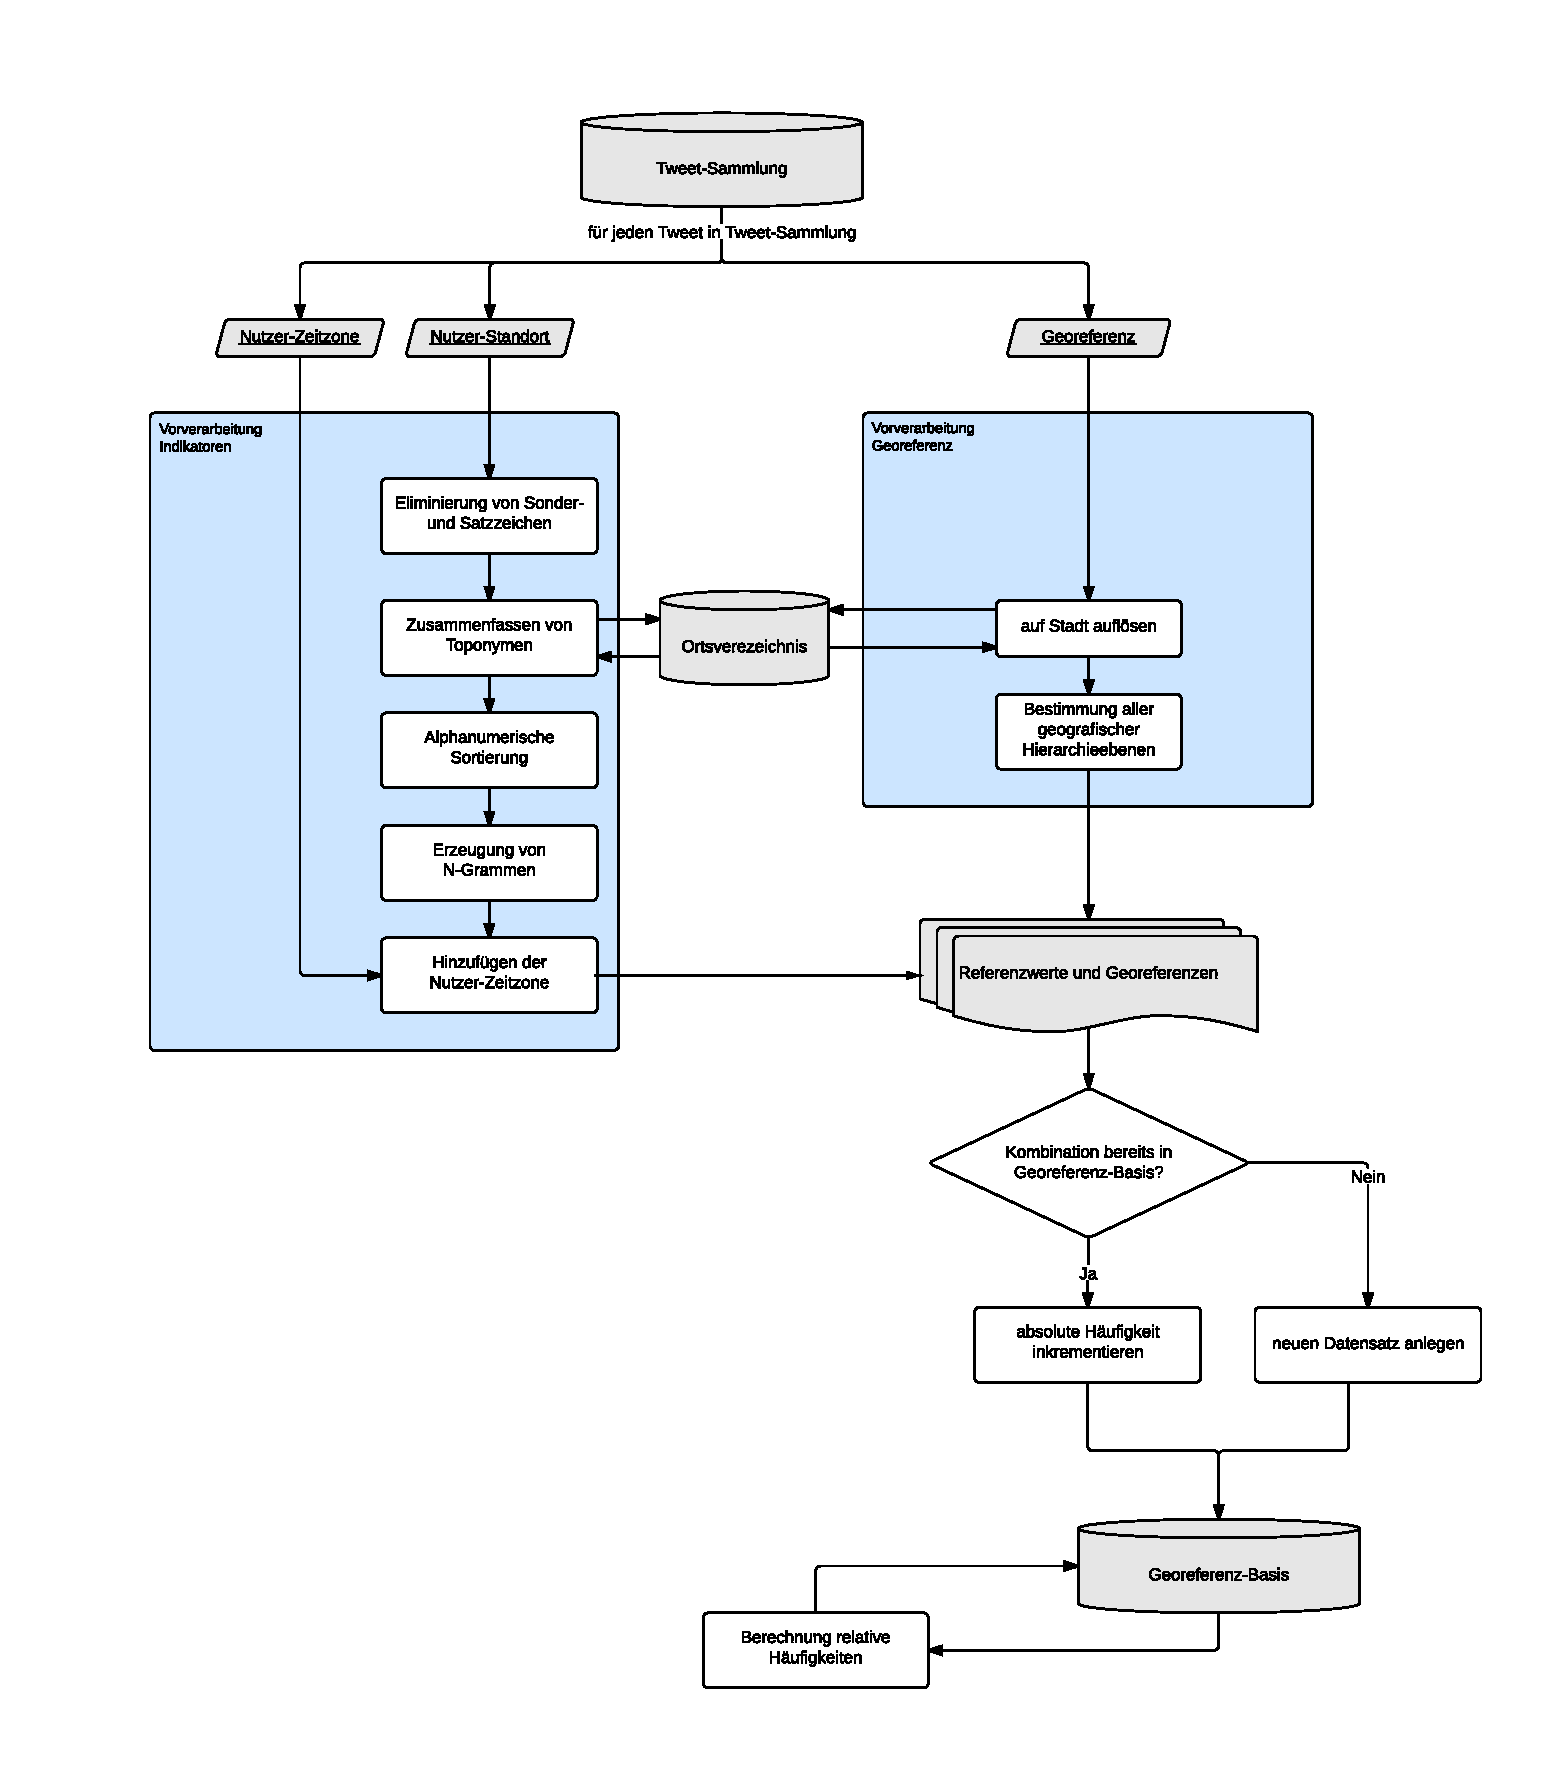
\includegraphics[scale=0.5]{einlernenAblauf.pdf}
						\caption{Ablaufplan einlernen}
						\label{img:einlernenAblauf}
					\end{center}
				\end{figure}


			Die Vorverarbeitung extrahiert dabei zusätzliche Informationen aus dem Nutzer-Standort.
			Durch die Bereiningung der Werte im Nutzer-Standort, die alphanumerische Sortierung, das identifzieren von Toponymen mit mehreren Worten und die darauffolgende Erzeugung von N-Grammen werden zusätzliche Informationen aus jedem Nutzer-Standort gewonnen.
			Die Nutzer-Zeitzone wird einbezogen um Doppeldeutigkeiten auflösen zu können.

			Durch die neue Datenstruktur, mit den absoluten Häufigkeiten und der abgebildeten geografischen Hierarchie, lassen sich nun tiefergehende Analysen durchführen um eine robuste Geolokalisierung zu ermöglichen. 
			Die absoluten Häufigkeiten geben dabei an wie oft ein Referenzwert in einer bestimmten Region vorkommt.

			Durch dieses Verfahren lässt sich eine Datenbasis erzeugen die domänenspezifische Eigenheiten, in Bezug auf die Verwendung spezieller Begriffe oder Formulierungen, berücksichtigt.
			Des weiteren werden Toponyme, die in Ortsverzeichnissen unter Umständen nicht hinterlegt sind, berücksichtigt.
			Auch geografische Indikatoren mit mittelbarem geografischen Bezug, zum Beispiel die Verwendung spezieller Begriffe in einer geografischen Region, können einbezogen werden. 

	\section{Geografischer Bezug der eingelernten Referenzwerte} \label{sec:geografischerBezug} 
			
		Die eingelernten Referenzwerte beinhalten alle Werte aus den Nutzer-Standorten der Tweet-Lerndaten.
		Es sind also auch Referenzwerte vorhanden die keinen geografischen Bezug haben.
		Es ist die Frage zu beantworten: Wie kann bestimmt werden ob ein Referenzwert geografischen Bezug hat oder nicht?
		Oder: Wie kann vermieden werden, dass ein Referenzwert, der keinen geografischen Bezug hat, zur Geolokalisierung genutzt wird?
		
		Dies ist wichtig, denn durch die Referenzwerte wird in der eigentlichen Geolokalisierung einem geografischen Indikator eine Georeferenz zugewiesen. 
		Wird einem geografischen Indikator durch einen Referenzwert ohne geografischen Bezug eine Georeferenz zugewiesen ist diese mit hoher Wahrscheinlichkeit fehlerhaft.
		Dies wiederum führt zu schlechten und unzuverlässigen Ergebnissen.
		Es muss also ein Verfahren gefunden werden um zu entscheiden ob die Referenzwerte einen geografischen Bezug haben oder nicht.

		Es ist zu beachten, dass die Vorverarbeitung keine Aussage zum geografischen Bezug macht, sondern vielmehr die Referenzwerte aus den Nutzer-Standorten extrahiert. 
		Dies soll sicherstellen, das möglichst viele Informationen aus den Nutzer-Standorten gezogen werden können und insbesondere keine Informationen verloren gehen.  
		
		Um zu entscheiden ob ein Referenzwert geografischen Bezug hat oder nicht wird die absolute Häufigkeit verwendet.
		Die absoluten Häufigkeiten geben an wie oft ein Referenzwert in einer bestimmten Region, zunächst in der Voronoi-Region der entsprechenden Stadt, vorkommt.			 
		Daraus kann nun ein geografischer Bezug abgeleitet werden.

		\subsection{Die absolute Häufigkeit als Hinweis auf geografischen Bezug zu Städten} 
			
			Eine hohe absolute Häufigkeit kann ein Hinweis auf den geografischen Bezug eines Referenzwertes darstellen. 
			Aufgrund der Eigenschaften des Nutzer-Standorts ist anzunehmen, dass in der Voronoi-Region einer Stadt der Name der zugehörigen Stadt häufig vorkommt.
			Dadurch kann eine Relevanz des Referenzwertes zu einer Stadt abgeleitet werden. 
			Tritt der Referenzwert nicht häufig auf, so ist er von nur wenigen Nutzern als Nutzer-Standort in einer Stadt angegeben worden und somit für die Stadt nicht relevant.
			In Abbildung \ref{img:ulIstanbulWalesZoom} sind die Tweets in denen "'Istanbul"' im Nutzer-Standort vorkommt aufgetragen.
			Es ist deutlich eine Häufung um die Stadt Istanbul zu erkennen. 
			Werden die Tweets rund um Istanbul nun auf die Stadt Istanbul abgebildet, wird die Kombination aus dem Referenzwert "'Istanbul"' und der Georeferenz Istanbul sehr häufig vorkommen.
			In den Nutzer-Standorten der Tweets rund um Istanbul taucht "'Istanbul"' tatsächlich 972 mal auf.
			Damit kann eine Gewisse Relevanz für den Referenzwert "'Istanbul"' zur Stadt Istanbul abgeleitet werden.

			\begin{figure}[!ht]
					\begin{center}
						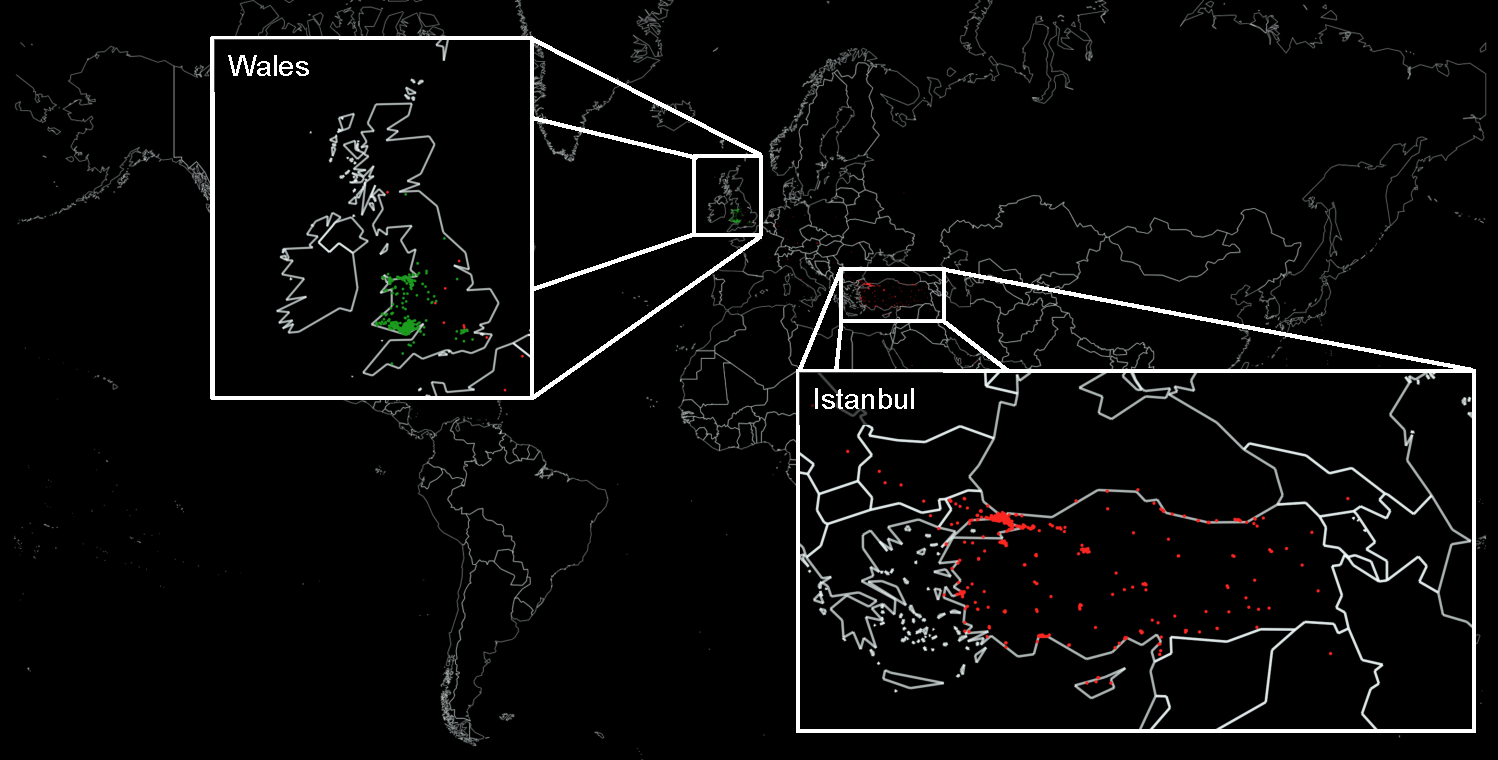
\includegraphics[scale=0.5]{ulIstanbulWalesZoom.pdf}
						\caption{}
						\label{img:ulIstanbulWalesZoom}
					\end{center}
			\end{figure}	

			Es kann also ein Schwellwert für die Häufigkeit eingeführt werden um Referenzwerte mit geografischem Bezug zu identifizieren.
			Allerdings garantiert die absolute Häufigkeit noch nicht, dass ein Referenzwert einen geografischen Bezug hat. 
			Es können auch Werte an einem bestimmten Ort häufig vorkommen, die keinen geografischen Bezug haben.
			Um dies erkennen zu können muss ein weiterer Wert berechnet werden.

		\subsection{Relative Häufigkeiten als Hinweis auf geografischen Bezug zu Städten}

			Betrachtet man die absoluten Häufigkeiten isoliert voneinander wird die Verteilung des Referenzwertes außer acht gelassen. 
			Ein Referenzwert kann eine gleichmäßige Verteilung über mehrere Städte aufweisen.
			Das bedeutet, der Referenzwert wird in vielen unterschiedlichen Städten benutzt. 
			Es können trotzdem Häufungen in Städten auftreten.
			Diese können sogar über einem gewählten Schwellwert für die absolute Häufigkeit liegen.
			Die Häufung kann jedoch relativ gesehen sehr gering sein.
			Dies ist ein Hinweis darauf das der Referenzwert keinen geografischen Bezug hat.
			Die relative Häufung sagt hier aus, das ein Referenzwert sehr verteilt auftritt. 
			Es ist also wichtig nicht nur die absoluten Häufigkeiten, sondern auch die relativen Häufigkeiten der Referenzwerte zu berücksichtigen.

			\subsubsection{Berechnung der relativen Häufigkeiten}  

				Um die relativen Häufigkeiten zu berechnen soll das Vorkommen eines Referenzwertes in einer Stadt, durch die Gesamtanzahl der Vorkommen des Referenzwertes geteilt werden.
				Damit erhält man den prozentualen Anteil der auf eine Stadt entfallenden Vorkommen eines Referenzwertes.
				Als Basis für diese Berechnung dienen die absoluten Häufigkeiten.

				Sei $(r_i,c_j)$ ein Datensatz der Georeferenz-Basis mit Referenzwert $r_i$ und Georeferenz $c_i$.
				Des weiteren liefert $H(r_{i},c_{j})$ die absolute Häufigkeit zu einem Referenzwert $r_i$ und einer Georefrenz $c_i$. 

				Damit kann die relative Häufigkeit $rel_{(r_i,c_j)}$ für jede Kombination $(r_i,c_j)$ durch die folgende Formel berechnet werden. 
				$n_c$ ist dabei die Anzahl aller Georeferenzen.

				\begin{equation}
					d_{r_i,c_j}=\frac{H(r_i,c_j)}{\sum^{n_c}_{j=0}{H(r_i,c_j)}}
				\end{equation}	

			\subsubsection{Beispiel} 

				"'La Plata"' tritt rund um die Stadt La Plata in Argentien 91 mal auf.
				Der Referenzwert "'La Plata"' hat offensichtlich einen geografischen Bezug zu einer Stadt. 

				Obwohl "'the"' keinen offensichtlichen geografischen Bezug hat ist die absolute Häufigkeit von 91 Vorkommen in Jakarta hoch.
				Der Schwellwert könnte nun aufgrund der Erfahrung mit dem Referenzwert "'La Plata"' auf 90 angesetzt werden.
				Dann würde davon ausgegangen werden, dass der Referenzwert "'the"' einen geografischen Bezug hat.
				Betrachtet man allerdings die Abbildung \ref{img:ULThe} fällt auf, dass Tweets mit dem Wert "'the"' im Nutzer-Standort sehr verteilt auf dem Globus auftreten.
				Im Gegensatz dazu tritt "'La Plata"' in den Nutzer-Standorten sehr konzentriert auf.
				In Abbildung \ref{img:ULlaPlata} wird die Verteilung von Tweets deren Verfasser "'La Plata"' im Nutzer-Standort enthalten dargestellt. 
				Es ist deutlich eine Häufung um die Stadt La Plata in Argentien zu erkennen, weltweit tritt der Referenzwert aber sehr selten auf.
\begin{figure} 
					\begin{center}
						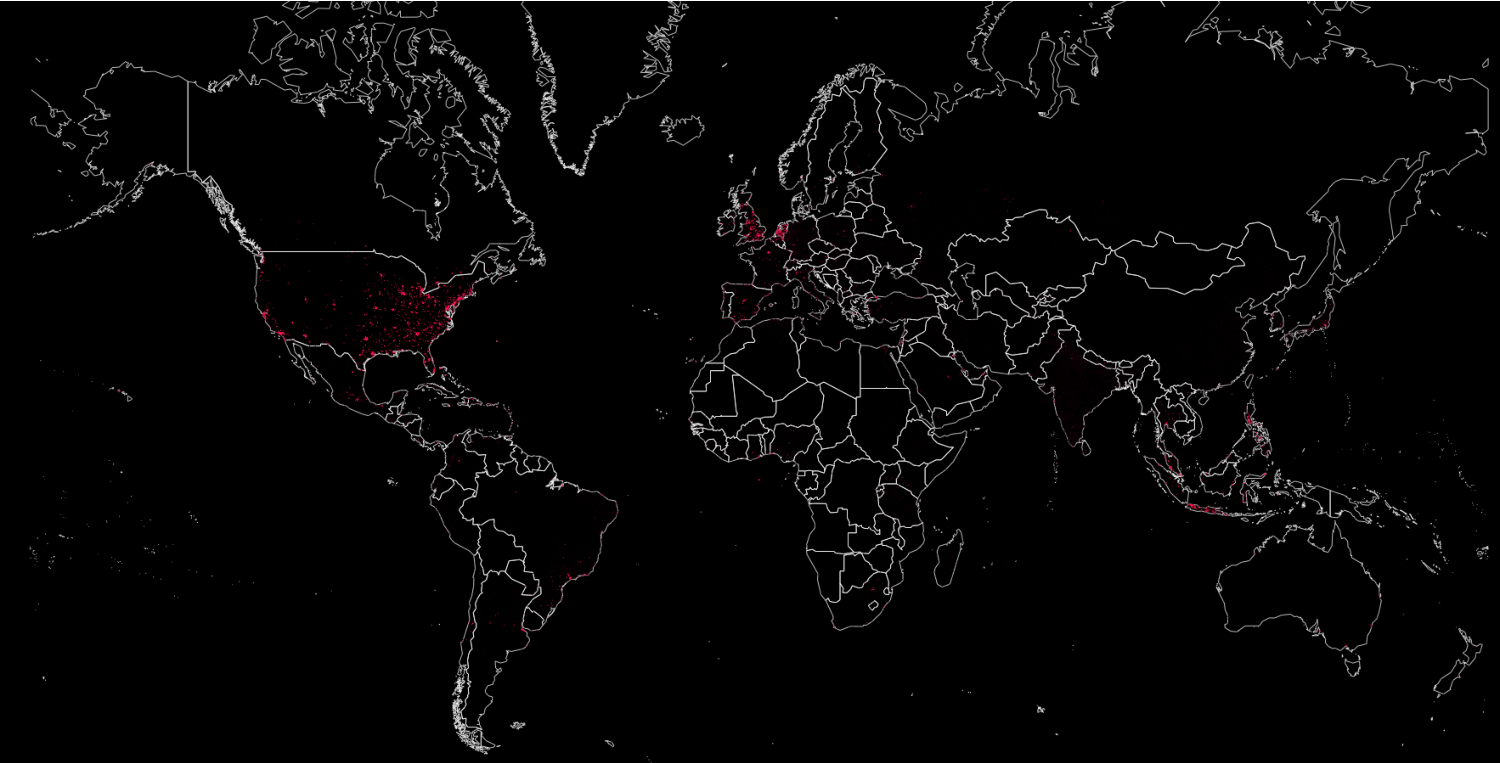
\includegraphics[scale=0.5]{ulTheG.pdf}
						\caption{Tweets mit Nutzer-Standort "'The"'}
						\label{img:ULThe}
					\end{center}
			\end{figure}
\begin{figure}
				\begin{center}
						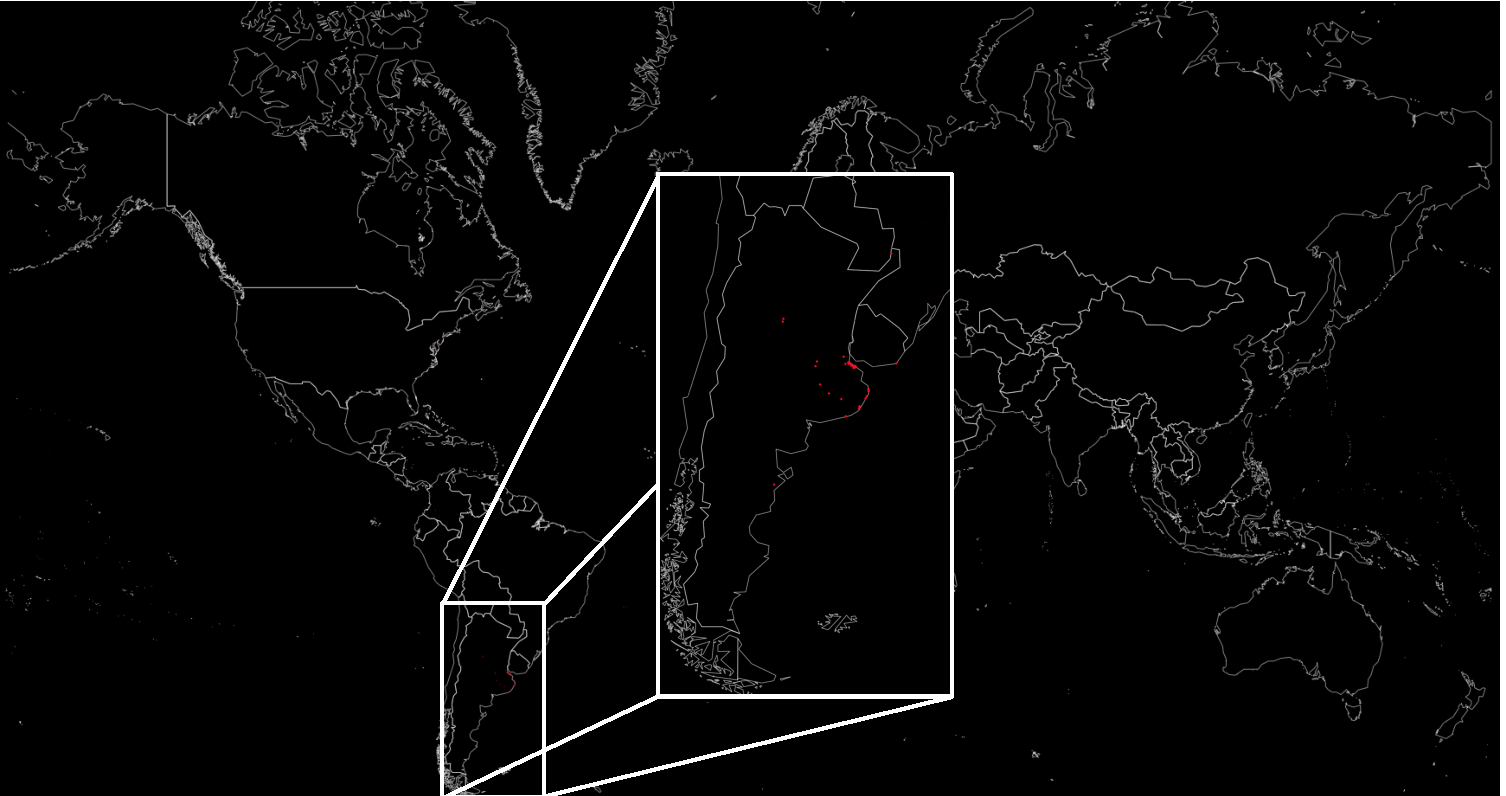
\includegraphics[scale=0.5]{ulLaPlataG.pdf}
						\caption{Tweets mit Nutzer-Standort "'La Plata"'}
						\label{img:ULlaPlata}
					\end{center}
			\end{figure}		
				
				Berechnet man nun die relativen Häufigkeiten kann dies abgebildet werden.
				In Tabelle \ref{tab:the} sind die zugeordneten Städte, die absoluten Häufigkeiten und die berechneten relativen Häufigkeiten für die Vorkommen des Wortes "'the"' aufgetragen. 
				Die Einträge sind absteigend nach dem Wert der relativen Häufigkeit sortiert.
				In Tabelle \ref{tab:the} werden nur die vier ersten Einträge dargestellt.  
				Insgesamt kam das Wort "'the"' in 2824 verschiedenen Städten vor.
				Dabei wurde es insgesamt 5764 mal verwendet. 
				Trotz der hohen absoluten Häufigkeit in Jakarta liegt die relative Häufigkeit bei lediglich 1,6\%.
				Aus den relativen Häufigkeiten lässt sich nun die, in Abbildung \ref{img:ULThe} vermutete, globale Verteilung ablesen.


				\begin{table}[h]
				\centering
				\caption{"'the"'}
				\label{tab:the}
				\begin{tabular}{|l|l|l|}
				\hline
				Stadt             & abs. Häufigkeit & rel. Häufigkeit in \% \\ \hline \hline
				Jakarta           & 91              & 1,6                       \\ \hline
				Singapore         & 27              & 0,5                       \\ \hline
				Bekasi            & 25              & 0,4                       \\ \hline
				Philadelphia      & 23              & 0,4                       \\ \hline
				... & ... & ... \\ \hline
				\end{tabular}
				\end{table}

				Die Verteilung erklärt sich dadurch, dass das Wort "'the"' im englischen sehr häufig auftritt.
				Englisch ist die internationale Verkehrssprache und wird dementsprechend global und sehr häufig verwendet.
				Dies spiegelt sich in der Verteilung der vorkommen auf dem Globus wieder.
				Die Häufung um Jakarta kann teilweise damit erklärt werden, dass sehr viele Tweets die in und um Jakarta abgesetzt werden eine Angabe von Längen- und Breitengrad aufweisen. 

				In Tabelle \ref{tab:laPlata} wird dieselbe Auswertung für "'La Plata"' dargestellt. 
				"'La Plata"' ist insgesamt 129 mal in 23 verschiedenen Städten aufgetaucht. 
				In der Stadt La Plata, in Argentien, kam es 91 mal vor.
				Dies entspricht einer relativen Häufigkeit von 70,5\%.

				\begin{table}[h]
				\centering
				\caption{"'La Plata"'}
				\label{tab:laPlata}
				\begin{tabular}{|l|l|l|}
				\hline
				Stadt            & abs. Häufigkeit & rel. Häufigkeit in \% \\ \hline \hline
				La Plata         & 91              & 70,5                      \\ \hline
				Villa Gesell     & 9               & 7,0                       \\ \hline
				Mar del Plata    & 5               & 3,9                       \\ \hline
				Quilmes          & 3               & 2,3                       \\ \hline
				... & ... & ... \\ \hline
				\end{tabular}
				\end{table}

				"'La Plata"' taucht erwartungsgemäß am häufigsten rund um die Stadt La Plata auf.  

				Es lässt sich also anhand der relativen Häufigkeiten ein geografischer Bezug des Referenzwertes nachweisen.
				Damit kann man zunächst bestimmen ob ein Referenzwert geografischen Bezug hat oder nicht.
				Die relativen Häufigkeiten können nach dem einlernen der Referenzwerte berechnet und in der Georeferenz-Basis hinterlegt werden.
				Mit Hilfe eines Schwellwertes für die relativen Häufigkeiten, kann nun bestimmt werden wann ein Referenzwert geografischen Bezug hat.

				Aber auch die ausschließliche Betrachtung der relativen Häufigkeiten reicht nicht aus um die geografische Relevanz nachzuweisen.
				Da die relativen Häufigkeiten basierend auf den Vorkommen des Referenzwertes berechnet werden sagen diese wiederum nichts über die absoluten Häufigkeit aus. 
				Kommt ein Referenzwert zwei mal in zwei verschiedenen Städten vor, liegen die jeweiligen relativen Häufigkeiten bei 50\%.
				Dies ist ein hoher Wert.
				Da der Referenzwert aber nur einmal vorkam, ist es sehr unwahrscheinlich das er einen geografischen Bezug hat.   

		\subsection{Geografischer Bezug zu Verwaltungseinheiten und Ländern} 

			Beim einlernen der Georeferenz-Basis werden durch die absoluten Häufigkeiten die Vorkommen pro Stadt gespeichert.
			Mit den daraus errechneten relativen Häufigkeiten kann nicht entschieden werden, ob für den Referenzwert eine globale Verteilung vorliegt oder ob der Referenzwert unter Umständen nur regional begrenzt, zum Beispiel in einem Land, auftritt.
			Für Referenzwerte die ein Land oder eine Verwaltungseinheit bezeichnen ist auf Städteebene eine geringe relative Häufigkeit zu erwarten.
			Diese Referenzwerte treten in einer größeren geografischen Region als der Voronoi-Region einer Stadt auf.
			Sie sind somit über mehrere Städte verteilt und werden auf Stadtebene einer geringe relative Häufigkeit aufweisen.
			Es ist beispielsweise zu erwarten das ein Ländername in den Nutzer-Standorten von Tweets aus dem gesamten Land auftritt.
			Durch die Unterteilung des Landes in Stadtgebiete wird der Wert sehr verteilt auf die Städte des Landes auftreten.

			Soll nun statt einer Stadt eine Verwaltungseinheit oder das Land als Georeferenz bestimmt werden, kann mit diesen absoluten Häufigkeiten auf Stadtebene keine Aussage über den geografischen Bezug gemacht werden. 
			
			Am folgenden Beispiel soll dieser Sachverhalt erläutert werden.

			In Abbildung \ref{img:ulIstanbulWalesZoom} sind in grün Tweets dargestellt, welche im Nutzer-Standort "'Wales"' enthalten.
			Wales entspricht einer Verwaltungseinheit erster Ordnung und gehört zu Großbritannien.
			Die Tweets sind in der gesamten geografischen Region, über die sich Wales erstreckt, verteilt.
			Außerhalb von Wales tritt "'Wales"' im Nutzer-Standort sehr selten auf.
			Die relativen Häufigkeiten auf Stadtebene werden in Tabelle \ref{tab:walesCity} dargestellt.
			Diese bestätigen eine Verteilung über eine größere geografische Region.
			Anhand der relativen Häufigkeiten kann aber nicht entschieden werden ob der Referenzwert global verteilt ist, oder in einer bestimmten geografischen Region, wie einem Land, auftritt. 
			"'Wales"' taucht in insgesamt 78 Städten 346 mal in Nutzer-Standorten auf.

			\begin{table}[h]
			\centering
			\caption{"'Wales"'}
			\label{tab:walesCity}
			\begin{tabular}{|l|l|l|}
			\hline
			Stadt      & abs. Häufigkeit & rel. Häufigkeit in \% \\ \hline \hline
			Cardiff    & 44 			 & 12,7 \\ \hline
			Newport    & 32 			 & 9,2  \\ \hline
			Carmarthen & 24 			 & 6,9  \\ \hline
			Swansea    & 18 			 & 5,2  \\ \hline
			...    & ... & ...  \\ \hline
			\end{tabular}
			\end{table}

			Die relative Häufigkeit von 12,7\% deutete eher darauf hin, dass "'Wales"' keinen geografischen Bezug aufweist.
			Auf Städteebene ist dies auch durchaus korrekt. 
			Allerdings kann aus diesen Ergebnissen kein geografischer Bezug zu einer der anderen geografischen Hierarchieebenen abgeleitet werden.
			Das Problem ist, dass Wales keinen geografischen Bezug zu einer Stadt aufweist, wohl aber zu einer Verwaltungseinheit erster Ordnung und daher zu einer geografischen Region. 

			Um dieses Problem lösen zu können müssen zu einem Referenzwert die relativen Häufigkeiten für die anderen geografischen Hierarchieebenen berechnet werden.
			Damit kann dann die Verteilung der Referenzwerte auf diese Hierarchieebenen betrachtet werden.
			
		\subsubsection{Berechnung der relativen Häufigkeiten zu Verwaltungseinheiten und Ländern} 

			Da zu jedem Referenzwert die zugehörigen Verwaltungseinheiten und Länder bekannt sind können die absoluten und relativen Häufigkeiten direkt aus der Georeferenz-Basis berechnet werden.

			Es müssen lediglich die absoluten und relativen Häufigkeiten aufsummiert werden, bei denen der Wert der jeweiligen geografischen Hierarchieebenen übereinstimmen.
			Im Beispiel aus Tabelle \ref{tab:walesCity} müssen alle absoluten und relativen Häufigkeiten derjenigen Städte aufsummiert werden, die in derselben Verwaltungseinheit erster Ordnung liegen.
			Betrachtet man die Verwaltungseinheiten zu allen Städten in denen "'Wales"' im Nutzer Standort vorkommt ergibt sich folgende Liste.

			\begin{enumerate}
				\item Wales 35
				\item England 30
				\item unterschiedliche Verwaltungseinheiten 13
			\end{enumerate}

			Aus dieser Betrachtung alleine lässt sich noch nicht entscheiden ob der Referenzwert "'Wales"' einen geografischen Bezug zu einer Verwaltungseinheit hat.
			Denn der Referenzwert kam sowohl in 30 Städten in England als auch in 30 Städten in Wales vor, was keinen signifikanten Unterschied darstellt. 
			Summiert man allerdings die Vorkommen und relativen Häufigkeiten pro Stadt auf ergibt sich daraus Tabelle \ref{tab:WalesVerw1}.

			\begin{table}[h]
			\centering
			\caption{"'Wales"'}
			\label{tab:WalesVerw1}
			\begin{tabular}{|l|l|l|}
			\hline
			Adm1 & abs. Häufigkeit & rel. Häufigkeit in \% \\ \hline \hline
			Wales                   & 298 & 86,1 \\ \hline
			England                 & 38  & 11,0 \\ \hline
			National Capital Region & 1   & 0,3  \\ \hline
			Stockholm               & 1   & 0,3  \\ \hline
			... & ... & ... \\ \hline
			\end{tabular}
			\end{table}  

			Die relative Häufigkeit von 86,1\% weißt nun deutlich darauf hin, dass der Referenzwert einen geografischen Bezug zu Wales hat.
			Mit diesem Vorgehen, kann der geografische Bezug eines Referenzwertes auf jeder der geografischen Hierarchieebenen untersucht werden.

			Analog können die Werte für die Verwaltungseinheit zweiter Ordnung und dem Land berechnet werden.
			Dieses Vorgehen ermöglicht es einen geografischen Bezug eines Referenzwertes auf jeder der geografischen Hierarchieebenen zu prüfen.

		\subsubsection{Fazit}

			Mit der absoluten Häufigkeit besteht ein erster Hinweis darauf ob ein Referenzwert geografischen Bezug hat oder nicht.
			Die alleinige Betrachtung der absoluten Häufigkeit lässt aber die Verteilung der Werte auf den jeweiligen geografischen Hierarchieebenen außer betracht.
			Mit den berechneten relativen Häufigkeiten können die Referenzwerte zusätzlich auf ihre Verteilung untersucht werden.
			Die relativen Häufigkeiten können nach dem Einlernen berechnet und in der Georeferenz-Basis gespeichert werden. 
			Während der Geolokalisierung kann dies absolute und relative Häufigkeit genutzt werden um die geografischen Indikatoren zu bestimmen. 

	\section{Verfahren zur Geolokalisierung am Beispiel von Twitter}

		In Kapitel \ref{sec:einlernen} wurde ein Verfahren zum einlernen der Georeferenz-Basis vorgestellt. 
		Im darauffolgenden Kapitel \ref{sec:geografischerBezug} wurde eine Möglichkeit vorgestellt wie der geografische Bezug der Referenzwerte untersucht werden kann.
		Dies soll hier genutzt werden um eine Georeferenz zu bestimmen. 

		Es soll nun das Verfahren zur Geolokalisierung eines Twitter-Nutzers vorgestellt werden.
		Dabei dient die Georeferenz-Basis und die in ihr abgelegten Werte als Basis für die Zuweisung einer Georeferenz.

		Zunächst werden aus dem Nutzer-Standort und der Nutzer-Zeitzone potenzielle geografische Indikatoren erzeugt.
		Dies geschieht analog zur Erzeugung von Referenzwerten beim einlernen der Georeferenz-Basis.
		Es werden also dieselben Vorverarbeitungsschritte für den Nutzer-Standort und die Nutzer-Zeitzone durchgeführt.
		Daraus resultiert eine Menge potenzieller geografischer Indikatoren.
		Die Werte der potenziellen geografischen Indikatoren werden nun in der Georeferenz-Basis nachgeschlagen. 
		Dabei werden alle Datensätze deren Referenzwerte mit den potenziellen geografischen Indikatoren korrespondieren zurückgegeben.
		Auf diesen Datensätzen erfolgt die weitere Verarbeitung und Bestimmung der wahrscheinlichsten Georeferenz.
		
		Es liegt nun eine Menge an Datensätzen aus der Georeferenz-Basis vor.
		Die Referenzwerte entsprechen dabei den potenziellen geografischen Indikatoren.
		Die absoluten und relativen Häufigkeiten werden für jeden Referenzwert separat analysiert.
		Das Ziel der Analyse ist es, die wahrscheinlichste Georeferenz zu ermitteln.

		In Abbildung \ref{img:ablaufGeolok} ist der gesamte Ablauf an einem Beispiel dargestellt.
		In den folgenden Abschnitten soll nun die Analyse genauer betrachtet werden.

			\begin{figure} 
			\begin{center}
						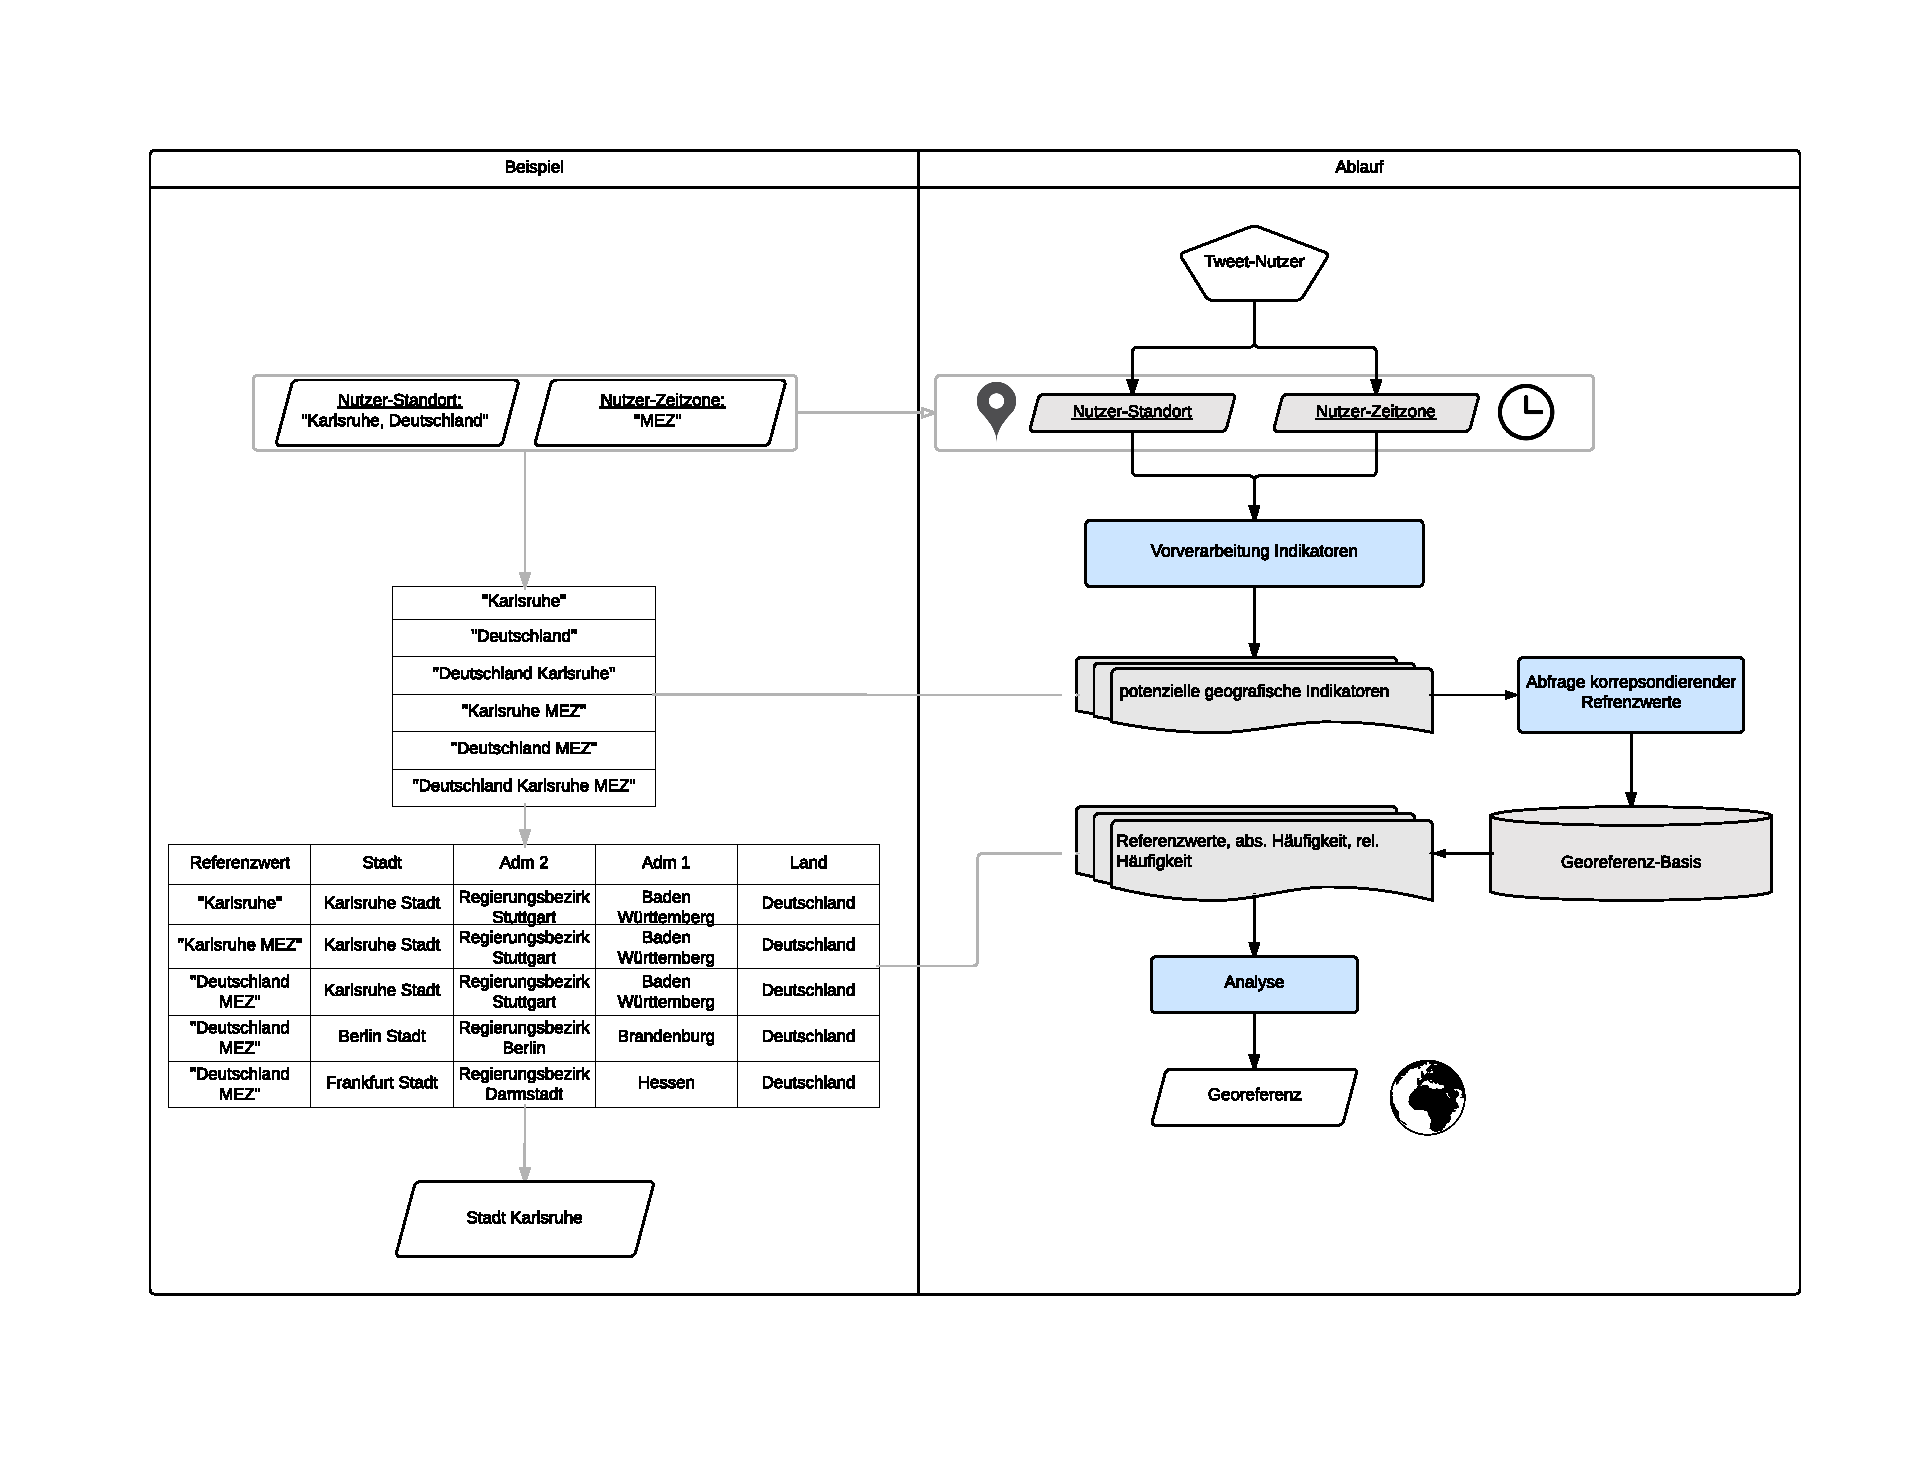
\includegraphics[scale=0.5]{geolokalisierungAllg.pdf}
						\caption{Ablauf der Geolokalisierung mit Beispiel}
						\label{img:ablaufGeolok}
					\end{center}
			\end{figure}	

		\subsection{Analyse}

			Die Analyse beinhaltet zwei Schritte. 
			Zuerst müssen diejenigen Referenzwerte gewählt werden, welche am wahrscheinlichsten einen geografischen Bezug haben.
			Dabei wird jeder Referenzwert separat betrachtet. 
			In einem nächsten Schritt wird derjenige Referenzwert gewählt, der unter den verbliebenen am wahrscheinlichsten die geografische Position des Nutzers beschreibt. 

			\subsubsection{Auswahl der Referenzwerte mit geografischem Bezug}

				Es können pro Referenzwert zunächst mehrere Datensätze vorliegen.
				Aus diesen sollen diejenigen gewählt werden, welche am wahrscheinlichsten einen geografischen Bezug aufweisen.
				Dazu werden sowohl die absoluten als auch die relativen Häufigkeiten genutzt. 
				Für jeden Referenzwert wird derjenige Datensatz gewählt, der die größte relative Häufigkeit $h_{rel}$ über einem Schwellwert $s_{rel}$ aufweist.
				Mit diesem Schwellwert lässt sich bestimmen wie verteilt der Referenzwert auftreten kann.
				Zusätzlich wird geprüft ob die absolute Häufigkeit ebenfalls über einem Schwellwert $s_{abs}$ liegt.
				Mit diesem Schwellwert lässt sich bestimmen wie häufig der Referenzwert an einer geografischen Position oder in einer geografischen Region auftreten muss. 

			\subsubsection{Bestimmung der wahrscheinlichsten Georeferenz} 

				Nun liegt wiederum eine Menge an Datensätzen vor.
				Jeder Referenzwert, und damit auch jeder potenzielle geografische Indikator, taucht nur noch ein mal auf. 

				Aus den verbliebenen Datensätzen soll nun die Georeferenz gewählt werden. 
				Dazu werden die relativen Häufigkeiten verglichen.
				Es wird der Datensatz mit der höchsten relativen Häufigkeit gewählt.
				Die Georeferenz dieses Datensatzes wird dann dem Twitter-Nutzer zugewiesen. 
				Damit wird der Referenzwert ausgewählt der die größte relative Häufigkeit aller untersuchten Referenzwerte aufweist. 

				Die Referenzwerte stellen NGramme dar, wie in der Vorverarbeitung in Unterkapitel \ref{subsec:VorverarbeitungStandortZeitzone} erläutert wird.
				Es werden hier also insbesondere auch Uni-, Bi- und Trigramme miteinander verglichen.
				Darauf soll nun eingegangen werden.

				\paragraph{Vergleich der relativen Häufigkeiten zu Uni- Bi- und Trigrammen}

					Jedes Element eines Bi- oder Trigrammes kann potenziell einen geografischen Bezug haben. 
					Umso mehr Elemente ein NGramm beinhaltet umso spezieller kann die Beschreibung des geografischen Objekts sein.
					Deshalb können NGramme mit einem höheren Grad ein Objekt genauer beschreiben als NGramme mit einem niedrigeren Grad.

					Allerdings können NGramme mit einem höheren Grad auch eine schlechtere Beschreibung darstellen. 
					Beispielsweise wenn das zusätzliche Element keinen geografsichen Bezug hat.

					Bei NGrammen mit einem Grad größer zwei können also zwei Fälle unterschieden werden.

					\begin{enumerate}
						\item Die Kombination aus den Elementen des NGrammes beschreibt einen Ort genauer
						\item Die Kombination aus den Elementen des NGrammes beschreibt einen Ort nicht genauer
					\end{enumerate}

					\subparagraph{Fall1} 

						Ein Beispiel für den ersten Fall ist der Nutzer-Standort "'york"' mit der Nutzer-Zeitzone "'eastern+time+us+canada"'. 
						Durch die Vorverarbeitung werden folgende potenzielle geografische Indikatoren erzeugt.
						\begin{enumerate}		
							\item york
							\item york \textit{eastern+time+us+canada}
						\end{enumerate}		

						Eine Stadt Namens York existiert sowohl in Grossbritannien als auch in den USA.
						Fragt man nun die beiden Referenzwerte in der Georeferenz-Basis ab erhält man folgende Werte:

							\begin{table}[h]
								\centering
									\caption{"'york"'}
									\label{tab:york}
									\begin{tabular}{|l|l|l|l|}
									\hline
									Referenzwert 				& Stadt  	& abs. Häufigkeit & rel. Häufigkeit in \% \\ \hline \hline
									York          				& York (GB) & 97              & 48,3       \\ \hline
									york eastern+time+us+canada & York (US) & 12              & 63,2        \\ \hline
									\end{tabular}
							\end{table}

							Die realtive Häufigkeit für york in Kombination mit der Zeitzone ist höher. 
							Die Zeitzone gibt zusätzliche Auskunft darüber welches York gemeint ist. 
							Die Kombination ist spezieller, kommt deshalb seltener vor und potenziell eher dort wo sie zutrifft. 
							In diesem Fall in York in den USA. 

							In den meisten Fällen beschreibt einer der beiden Indikatoren eine größere geografische Region wie beispielsweise einen Bundesstaat der USA.
							Wird ein weiterer Wert, beispielsweise ein Städtename hinzugenommen, wird die Angabe des Ortes genauer. 
							Die Wahrscheinlichkeit, dass diese Kombination ausserhalb des Ortes auftritt wird geringer. 

					\subparagraph{Fall 2}

						Hier können wiederum 2 Fälle unterschieden werden.

						\begin{enumerate}
							\item Beide Elemente beziehen sich auf unterschiedliche geografische Objekte
							\item Nur ein Element hat geografischen Bezug das andere nicht 
						\end{enumerate}

						Wenn zu einem Referenzwert mit geografischem Bezug ein Element hinzugefügt wird, welches keinen geografischen Bezug hat, beschreibt dies den Ort nicht genauer.
						Es ist zu erwarten, dass die Kombination der Elemente sehr selten vorkommt oder sehr verteilt ist. 
						Ist die Kombination verteilter, so ist der relative Wert geringer als der des einzelnen Referenzwertes mit geografischem Bezug.
						Ist die Kombination seltener kann der Referenzwert bereits durch den Schwellwert $s_{abs}$ aussortiert werden.		

						Wenn zu einem Referenzwert mit geografischem Bezug ein Element hinzugefügt wird, welches zwar geografischen Bezug hat, aber dieses sich auf ein anderes geografisches Objekt bezieht ist dasselbe Verhalten zu erwarten.
						
			\subsubsection{Wahl der Schwellwerte}

				Die Wahl der beiden Schwellwerte ist abhängig von den Anforderungen.
				Dabei ist die gewünschte geografische Hierarchie der zurückgegeben Georeferenz ein Faktor.
				Und die gewünschte Genauigkeit und Trefferquote.
				
				\paragraph{Gewünschte Hierarchieebene der Georeferenz}

					Umso größer die betrachtete geografische Region ist, umso weniger Möglichkeiten zur Einteilung gibt es.
					Auf Städteebene gibt es 23322 verschiedene geografische Regionen. 
					Für jede Stadt mit mehr als 15000 Einwohnern existiert dabei eine Region.
					Diese Städte verteilen sich auf 234 verschiedene Länder.
					Dieselbe Menge an Referenzwerten, verteilt sich auf Länderebene also auf weniger geografische Regionen. 
					Dadurch werden die Werte der relativen Häufigkeit und der absoluten Häufigkeit insgesamt größer.
					Relativ zueinander werden allerdings nach wie vor Referenzwerte mit geografischem Bezug größer sein als Referenzwerte ohne geografischen Bezug.

					Es müssen also für jeder geografsiche Hierarchieebene geeignete Schwellwerte $s_{rel}$ und $s_{abs}$ gefunden werden.

				\paragraph{Genauigkeit und Trefferquote} 

					Der zweite Faktor ist die gewünschte Trefferquote und die Genauigkeit.

					Umso niedriger der Schwellwert $s_{rel}$ ist, umso größer wird die Wahrscheinlichkeit Referenzwerte zu wählen die keinen geografischen Bezug haben.
					Daraus resultieren mehr fehlerhafte Zuordnungen einer Georeferenz.
					Wodurch die Genauigkeit schlechter wird.
					Dadurch können allerdings mehr Georeferenzen zugeordnet werden, wordurch die Trefferquote verbessert wird.
					Umso höher der Schwellwert $s_{rel}$ gewählt wird umso mehr Referenzwerte mit geografischem Bezug werden verworfen.
					Die Wahrscheinlichkeit, dass die gewählten Referenzwerte tatsächlich geografischen Bezug haben ist allerdings höher.
					Dadurch können weniger Georeferenzen zugeordnet werden.
					Somit sinkt die Trefferquote.
					Allerdings sind die zugewiesenen Georeferenzen sicherer womit die Genauigkeit steigt.

					Der Schwellwert $s_{abs}$ vermeidet, dass Refrenzwerte gewählt werden die eine hohe realtive Häufigkeit aufweisen aber aufgrund ihrer geringen Vorkommen nicht relevant sind.
					Die Auswirkungen der Wahl des Schwellwertes $s_{abs}$ verhalten sich Analog zum Schwellwert $s_{rel}$.

				\paragraph{Fazit}

					Die Wahl der Schwellwerte hängt zum einen von der Hierarchieebene und zum anderen von den Anforderungen an die Genauigkeit und die Trefferquote ab.
					In Bezug auf die geografischen Hierarchieebenen sind lediglich separate Schwellwerte für jede geografischen Hierarchieebenen zu bestimmen, da die relativen und absoluten Häufigkeiten sich insgesamt verändern.
					Bezüglich der Genauigkeit und der Trefferquote ist ein Kompromiss zwischen den beiden Werten einzugehen. 
					Die Verbesserung der Trefferquote geht mit einer Verschlechterung der Genauigkeit einher und umgekehrt.
					Es kann also entweder ein Kompromiss gefunden werden der ein Optimum für beide Werte darstellt. 
					Oder einer der Werte wird optimiert. 
			
		



	

%!TEX root = ../document.tex
\chapter{Implementierung} 
	
	\todo{chap:Implementierung} 
	Im Rahmen dieser Diplomarbeit ist eine Referenzimplementierung des vorgestellten Verfahrens entstanden.
	In Auszügen soll die Referenzimplementierung hier vorgestellt werden. 
	Hierbei sollen insbesondere Probleme bei der Umsetzung betrachtet werden, und wie diese gelöst wurden. 
	Damit soll die Möglichkeit gegeben werden, in eigenen Implementierungen die Probleme frühzeitig zu erkennen und zu vermeiden.  



	\section{Verwendete System}
		\todo{chap:Implementierung sec: Verwendete Systeme}
		CSharp, SQL Server, IIS Server 

	\section{Architektur}
		
		\todo{chap:Implementierung sec: Architektur}
		Allgemeine Architektur der Referenzimplementierung.
		Klassnediagramm
		Sequenzdiagramm

		\subsection{Präprozessorverarbeitung}
			
			\todo{chap:Implementierung sec: Architektur subsec: Präprozessorverarbeitung}
			Warum Präprozessoren -> schnelleres ändern der Vorverarbeitung.
			Durchreichen des Tweets und Verarbeitung durch Präprozessoren.

	\section{Datenbank}
		
		\todo{chap:Implementierung sec: Datenbank}
		Datenbankschema.
		Geography Datatypes and Methods.
		Nearest Neighbour search SQL Server

	\section{Oberfläche zur manuellen Zuordnung von Georeferenzen}

		\todo{chap:Implementierung sec: Oberfläche zur manuellen Zuordnung von Georeferenzen}
		Kurz Oberfläche vorstellen plus verwendete Technologien. 

	\section{Probleme und Fallstricke} 

		\todo{chap:Implementierung sec: Probleme und Fallstricke}




%!TEX root = ../document.tex
\chapter{Leistungsbewertung} 



	\todo{chap:Grundlagen sec:Precision Recall}

	\todo{chap:Grundlagen sec:Konfidenzen}   

	\section{Bestimmung Schwellwerte} 
		
		\todo{chap:Lesitungsbewertung sec:Bestimmung Schwellwerte} 
		Ergebnisse Kontrolldaten.
		Angabe Schwellwerte über Random 2D Array. 
		Darstellung in Matlab.
		Maximum finden. 

	\section{Naiver Ansatz}
		
		\todo{chap:Lesitungsbewertung sec:Naiver Ansatz} 
		Im Vergleich zu einem naiven Ansatz.
		Google Maps API V3 ohne Vorverarebitung 
		Precision/Recall. 


	\section{Vergleich zu früheren Ansätzen auf Nutzer-Standort}
		
		\todo{chap:Lesitungsbewertung sec:Vergleich zu früheren Ansätzen auf Nutzer-Standort} 

	\section{Vergleich zu früheren Ansätzen NLP}
		
		\todo{chap:Lesitungsbewertung sec:Vergleich zu früheren Ansätzen NLP}

	\section{Fazit}   

		\todo{chap:Lesitungsbewertung sec:Fazit}

%!TEX root = ../document.tex
\chapter{Schlussfolgerungen, Ausblick und Fragen} 

%!TEX root = ../document.tex
\chapter{Zusammenfassung} 

	Über das Twitter-Netzwerk werden täglich mehr als 500 Millionen Tweets und damit Informationen verbreitet und weitergegeben. 
	Die Tweets sind zum Größtenteil öffentlich zugänglich. 
	Aus dieser enormen Informationsmenge lassen sich Erkenntnisse ableiten, mit denen politische und wirtschaftliche Entscheidungsprozesse unterstützt und verbessert werden können. 
	Im Katastrophenfall können schnelle Informationen den Entscheidungsträgern wichtige Hinweise liefern, die notwendigen, präventiven Schutzmaßnahmen einzuleiten.
	Um die Informationen effizient nutzen zu können, müssen den Tweets geografische Koordinaten zugeordnet werden.
	Allerdings weisen nur ca. 1\% der Twitter-Nachrichten geografische Koordinaten auf.

	Mit dem in dieser Arbeit vorgestellten Verfahren ist es möglich, Tweets über Angaben im Nutzer-Standort und der Nutzer-Zeitzone einer geografischen Position zuzuordnen.
	Die Geolokalisierung von Tweets erfolgt über eine Wissensdatenbank (Georeferenz-Basis), die mit einem Lerndatensatz bestehend aus Tweets mit den benötigten Informationen eingelernt wird. 
	Aus diesen Lerndatensätzen werden Referenzwerte extrahiert, denen eine Georeferenz zugeordnet wird.
	Damit kann das Vorkommen der Referenzwert an einer geografischen Postion oder in einer geografischen Region erfasst und in der Georeferenz-Basis gespeichert werden.
	Die Georeferenz-Basis stellt eine Art probabilistisches Sprachmodell für geografische Positionen oder Regionen dar.
	Soll ein Tweet lokalisiert werden, werden aus dessen Nutzer-Standortfeld und Nutzer-Zeitzone potenzielle geografische Indiaktoren erzeugt.
	Durch eine Abfrage dieser potenziellen geografischer Indikatoren an diese Georeferenz-Basis werden diejenigen Datensätze zurückgegeben, für die der Referenzwert mit einem der potenziellen geografischen Indikatoren korrespondiert.
	Es liegt dann eine Menge an möglichen Georeferenzen zu dem Tweet vor.
	Durch eine Analyse der Verteilung der Referenzwerte wird dann die wahrscheinlichste Georeferenz gewählt.
	Durch die Angabe von Schwellwerten für die Verteilung kann das Verfahren justiert werden, für eine gegeben Anforderung an die Precision können entsprechende Schwellwerte gewählt werden.
	Der Einfluss auf den Recallwert ist vorhersehbar.
	Dies macht das Verfahren beherrschbar und die Ergebnisse vorhersagbar.
	Des weiteren kann durch die Wahl der Schwellwerte eine Optimierung des Trade-Off durchgeführt werden um die bestmöglichen Ergebnisse zu erzielen.
	Es kann zudem bestimmt werden, ob das Ergebnis eine Stadt(geografische Koordinaten), Verwaltungseinheit erster Ordnung(beispielsweise ein Bundesland), Verwaltungseinheit zweiter Ordnung(beispielsweise Regierungsbezirke) oder ein Land sein soll. 
	Das Wissen über den gewünschten Rückgabewert wird einbezogen, um die Ergebnisse zu optimieren.
	Es werden keine Einschränkungen bezüglich der verwendeten Sprache oder des verwendeten Alphabets gemacht.
 	
	Es konnten folgende Ergebnisse erzielt werden. 
	Für den Rückgabewert Stadt wurde eine maximale Ergebnismenge von 79,1\% bei einem Median der Fehlerdistanzen von 20,43km erzielt.
	Der beste Wert für den Median der Fehlerdistanzen liegt bei 3,24km mit einer Ergebnismenge von 0,99\%.
	Die Optimierung des Median zieht eine Absenkung der Ergebnismenge nach sich. 
	Durch die Evaluierung wurden Schwellwerte für den besten möglichen Trade-Off zwischen Median und Ergebnismenge ermittelt.
	Dadurch konnte eine Ergebnismenge von 53,21\% und ein Median von 9,17km erreicht werden. 
	Im Vergleich zum besten Wert des Median der Fehlerdistanzen (3,24km) konnte durch eine moderate Änderung des Median die Ergebnismenge um ca. das 50-fache (von ) gesteigert werden.
	Auf den restlichen geografischen Hierarchieebenen wurden als Kennzahlen Precision und Recall verwendet.
	Für die Verwaltungseinheit zweiter Ordnung konnte für den besten Trade-Off eine Precision von 77\% bei einem Recall von 12\%, für die Verwaltungseinheit zweiter Ordnung lag der beste Trade-Off eine Precision von 80\% bei einem Recall von 54\%.
	Auf Länderebene lag der beste Wert für die Precision bei 99\% bei einem Recall von 23\%, dies bedeutet nahezu alle Tweets, denen durch die Geolokalisierung ein Land zugeordnet werden konnte, wurden dem korrekten Land zugeordnet.
	Der beste Trade-Off lag hier bei einer Precision von 92\% und einem Recall von 84\%.





%!TEX root = ../document.tex
\chapter{Ideen und Notizen}

	\section{Stakeholder analyse}
	Welche potenziellen Stakeholder profitieren von der Arbeit? 
	Was benötigt jeder dieser Stakeholder? Bedürfnisse analysieren und Begründen.  

	\begin{enumerate}
		\item Marketing Professionals
		\item Statistiker allgemein
		\item Sozialwissenschaftler -> Analyse von Informationsströmen
	\end{enumerate}


	\section{Fragen an Matthias}
		\subsection{Strukturell}
			\begin{enumerate}
				\item Soll ich noch auf die Messung eines Informationsflusses eingehen? 
				Wenn ich keine Informationsflüsse untersuche hängt dieses Thema ein wenig in der Luft.
				\item ???  
			\end{enumerate}

		\subsection{Inhalt} 


	\section{Ideen}


	\begin{enumerate}
		\item \todo{In Einleitung} Voraussetzungen zur Anwendung des Verfahrens
		\begin{enumerate}
			\item Lerndaten mit konkreten geografischen Angaben
			\item Indikatoren in Lerndaten, welche auch in Datensätzen ohne konkrete geografische Angaben vorkommen (hier eventuelle Diskrepanzen zwischen geogetaggten und nicht geogetaggten tweets + Mentalität in bestimmten Ländern)
			\item Indikatoren mit geografischem Bezug, oder hinreichendem geografischen Bezug, Mittelbar oder unmittelbar
		 \end{enumerate}
		 \item Auf Jargon Namen für Städte eingehen, wie bspsw. the big apple -> New York City 
		 \item Landesgrenzen-Problematik wird durch meine Lösung obsolet -> auf stakeholder eingehen
		 \item \todo{Korrelation zwischen Lokalisierungungssicherheit und tatsächlichem Match berechnen} Wahrscheinlichkeiten für korrekte Lokalisierung kann angegeben und justiert werden 
		 \item Wenn Wahrscheinlichkeiten auf best. Ebene nicht hoch genug dann verschieben auf Admin2 -> Admin1 -> Länderebene
		 \item mit vorherigem werden Unsicherheiten bei Lokalisierung abgebildet (Wichtig für Informationsflüsse) 
		 \item  
	\end{enumerate}


	\section{Datenbasis}
		\begin{enumerate}
			\item Welche Datenbasis wurde genutzt 
				\begin{enumerate}
					\item Streaming API
					\item Is the Sample good enough (Morstatter et al 13)
					\item When is it biased? (Morstatter et al)
					\item How does the Data sampling Startegy Impact the Discovery of Information Diffusion in Social Media (De Choudhurry, 1)
				\end{enumerate}
			\item Lerndatensatz
			\item Kontrolldatensatz
			\item Manuell getaggter Datensatz
			\item Google Maps getaggter Datensatz
		\end{enumerate}			
	 
	 \section{Vorteile neuer Ansatz bei Mapping auf Geografische Daten}	
	Notwendigkeit/Vorteile von Hierarchiebeziehungen im Mapping auf Geograohie Daten
	
\nocite{*}								% Alle Refenezen werden aufgelistet
\bibliographystyle{alpha} 				% Layout Stil der Bibliographie
 \bibliography{bibtex/dipl}                     % Literatur Datei einbinden
			
\end{document}
